\graphicspath{{chapt_dutch/}{intro/}{chapt2/}{chapt3/}{chapt4/}{chapt5/}{chapt6/}{chapt7/}}

% Header
\renewcommand\evenpagerightmark{{\scshape\small Appendix D}}
\renewcommand\oddpageleftmark{{\scshape\small Impact of systematic uncertainties}}

\renewcommand{\bibname}{References}

\hyphenation{}

\chapter[Impact of systematic uncertainties]%
{Impact of systematic uncertainties}\label{app5}
%
This appendix contains plots that show the impact of systematic uncertainties on the results.
Section~\ref{sec:single_unc} shows the impact that single uncertainties have on the combined obtained signal strength, whereas section~\ref{sec:group_unc} shows how different groups of systematic uncertainties contribute to the expected upper limits on the coupling strength.

\subsection{Single uncertainties}
\label{sec:single_unc}

\begin{figure}[!Hhtb]
\centering
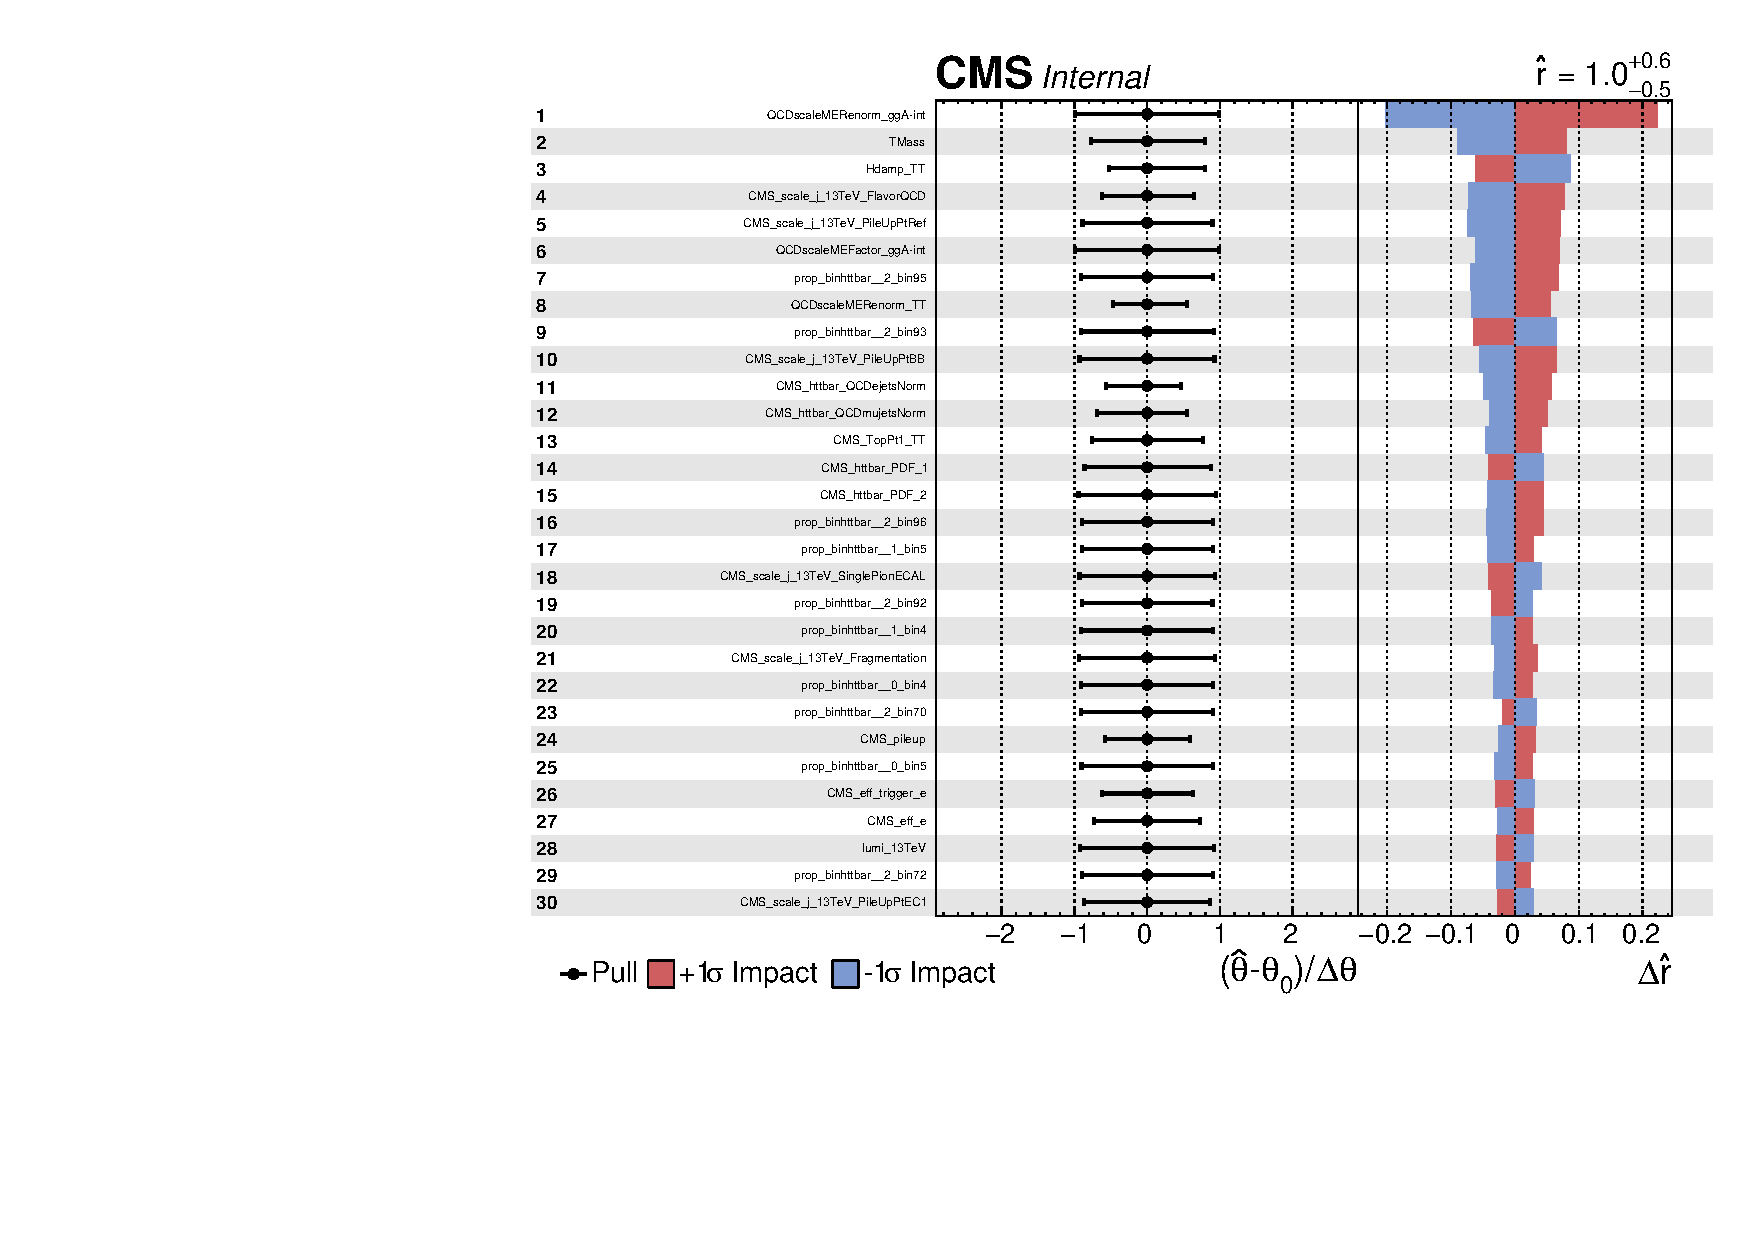
\includegraphics[width=0.85\textwidth,keepaspectratio=true]{fig/app5/impacts/impacts_400.pdf}
\caption{Impacts of systematic uncertainties on obtained coupling strength modifier for a 400\,GeV pseudoscalar with a relative width of 2.5\%. The impacts are shown for the Asimov dataset with a coupling strength modifier corresponding to the central expected limit. The right-hand side of the plot shows the relative variation of the obtained coupling strength under variations of the considered nuisance parameter within $\pm 1$ s.d.\ of its post-fit uncertainty (the so-called impact). The 30 uncertainties with the largest impact are shown. In addition, the post-fit value of the nuisance parameter and its uncertainty is shown on the left-hand side.}
\label{fig:impacts_m400}
\end{figure}

\begin{figure}[!Hhtb]
\centering
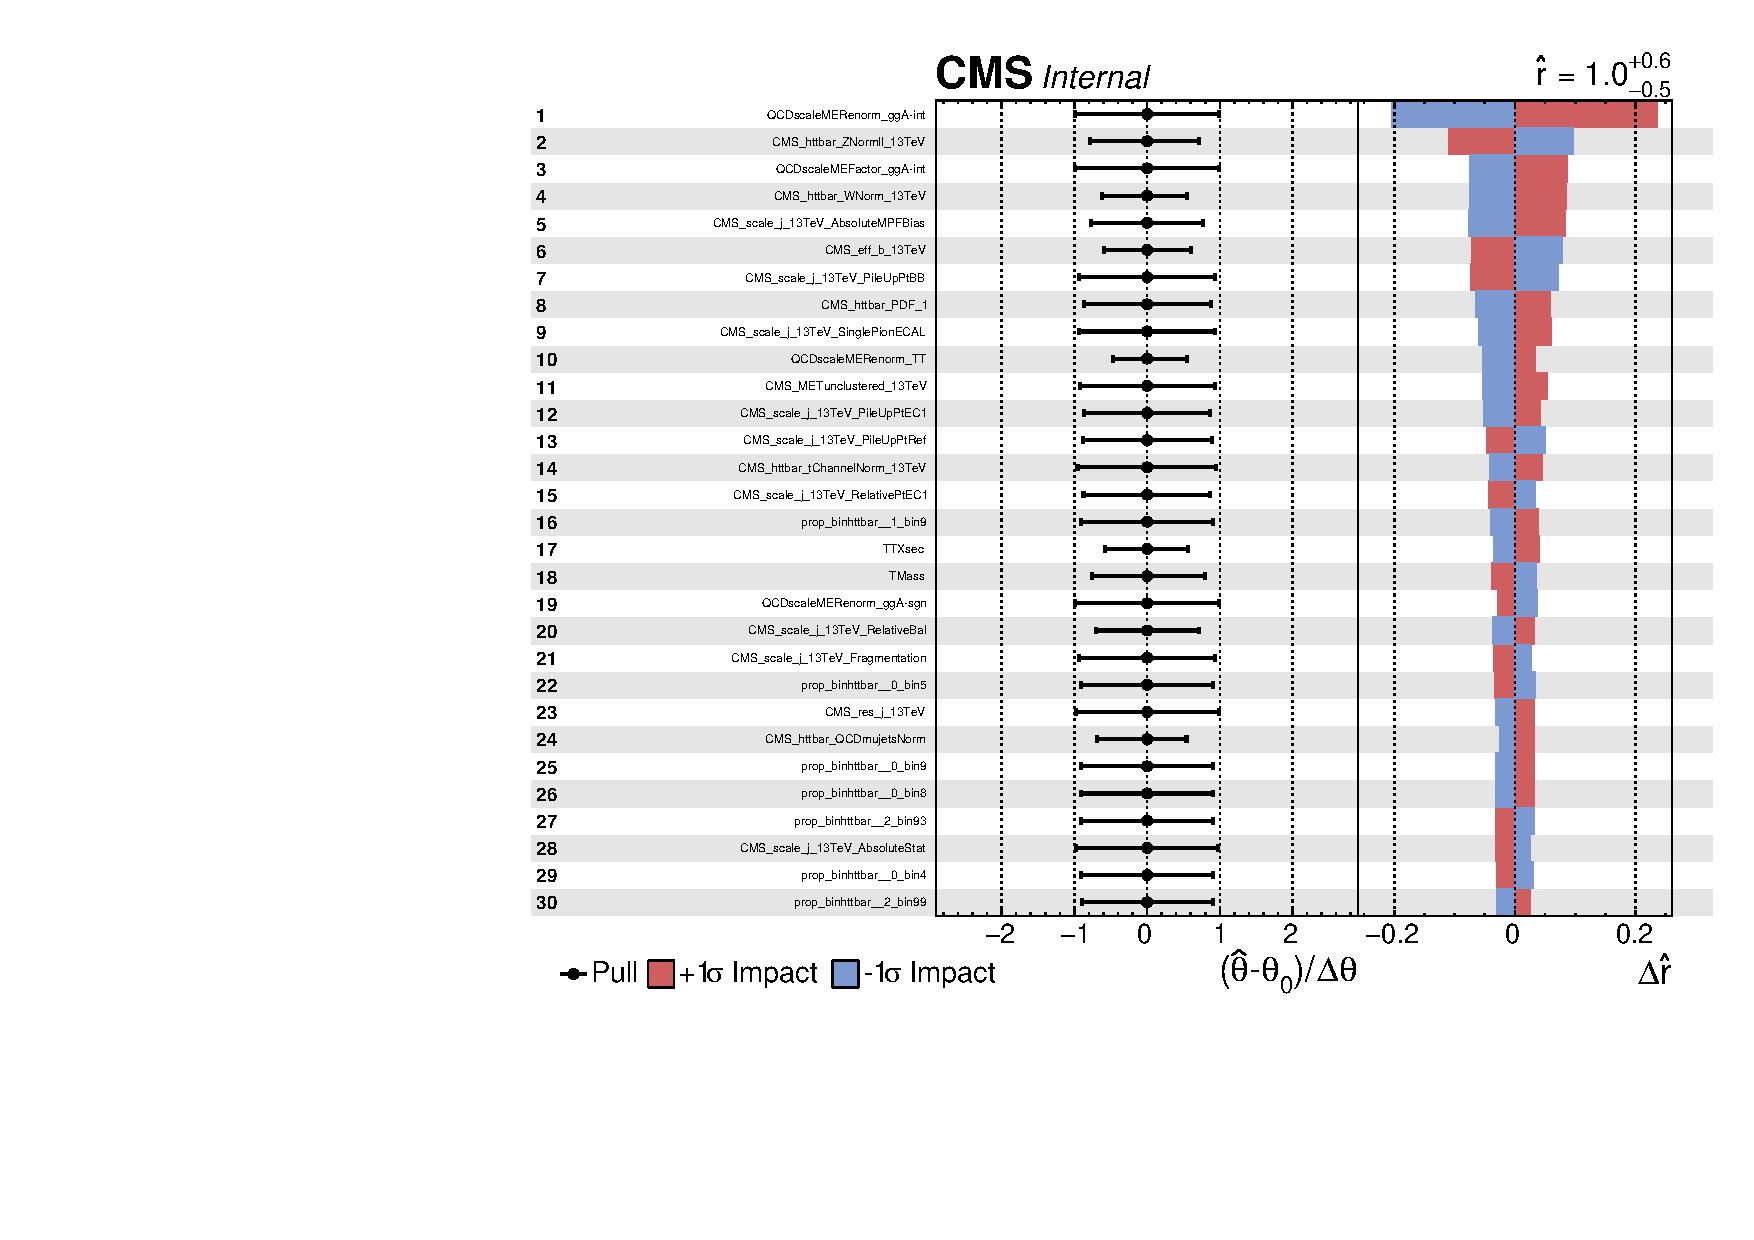
\includegraphics[width=0.85\textwidth,keepaspectratio=true]{fig/app5/impacts/impacts_500.pdf}
\caption{Impacts of systematic uncertainties on obtained coupling strength modifier for a 500\,GeV pseudoscalar with a relative width of 5\%. The impacts are shown for the Asimov dataset with a coupling strength modifier corresponding to the central expected limit. The right-hand side of the plot shows the relative variation of the obtained coupling strength under variations of the considered nuisance parameter within $\pm 1$ s.d.\ of its post-fit uncertainty (the so-called impact). The 30 uncertainties with the largest impact are shown. In addition, the post-fit value of the nuisance parameter and its uncertainty is shown on the left-hand side.}
\label{fig:impacts_m500}
\end{figure}

\begin{figure}[!Hhtb]
\centering
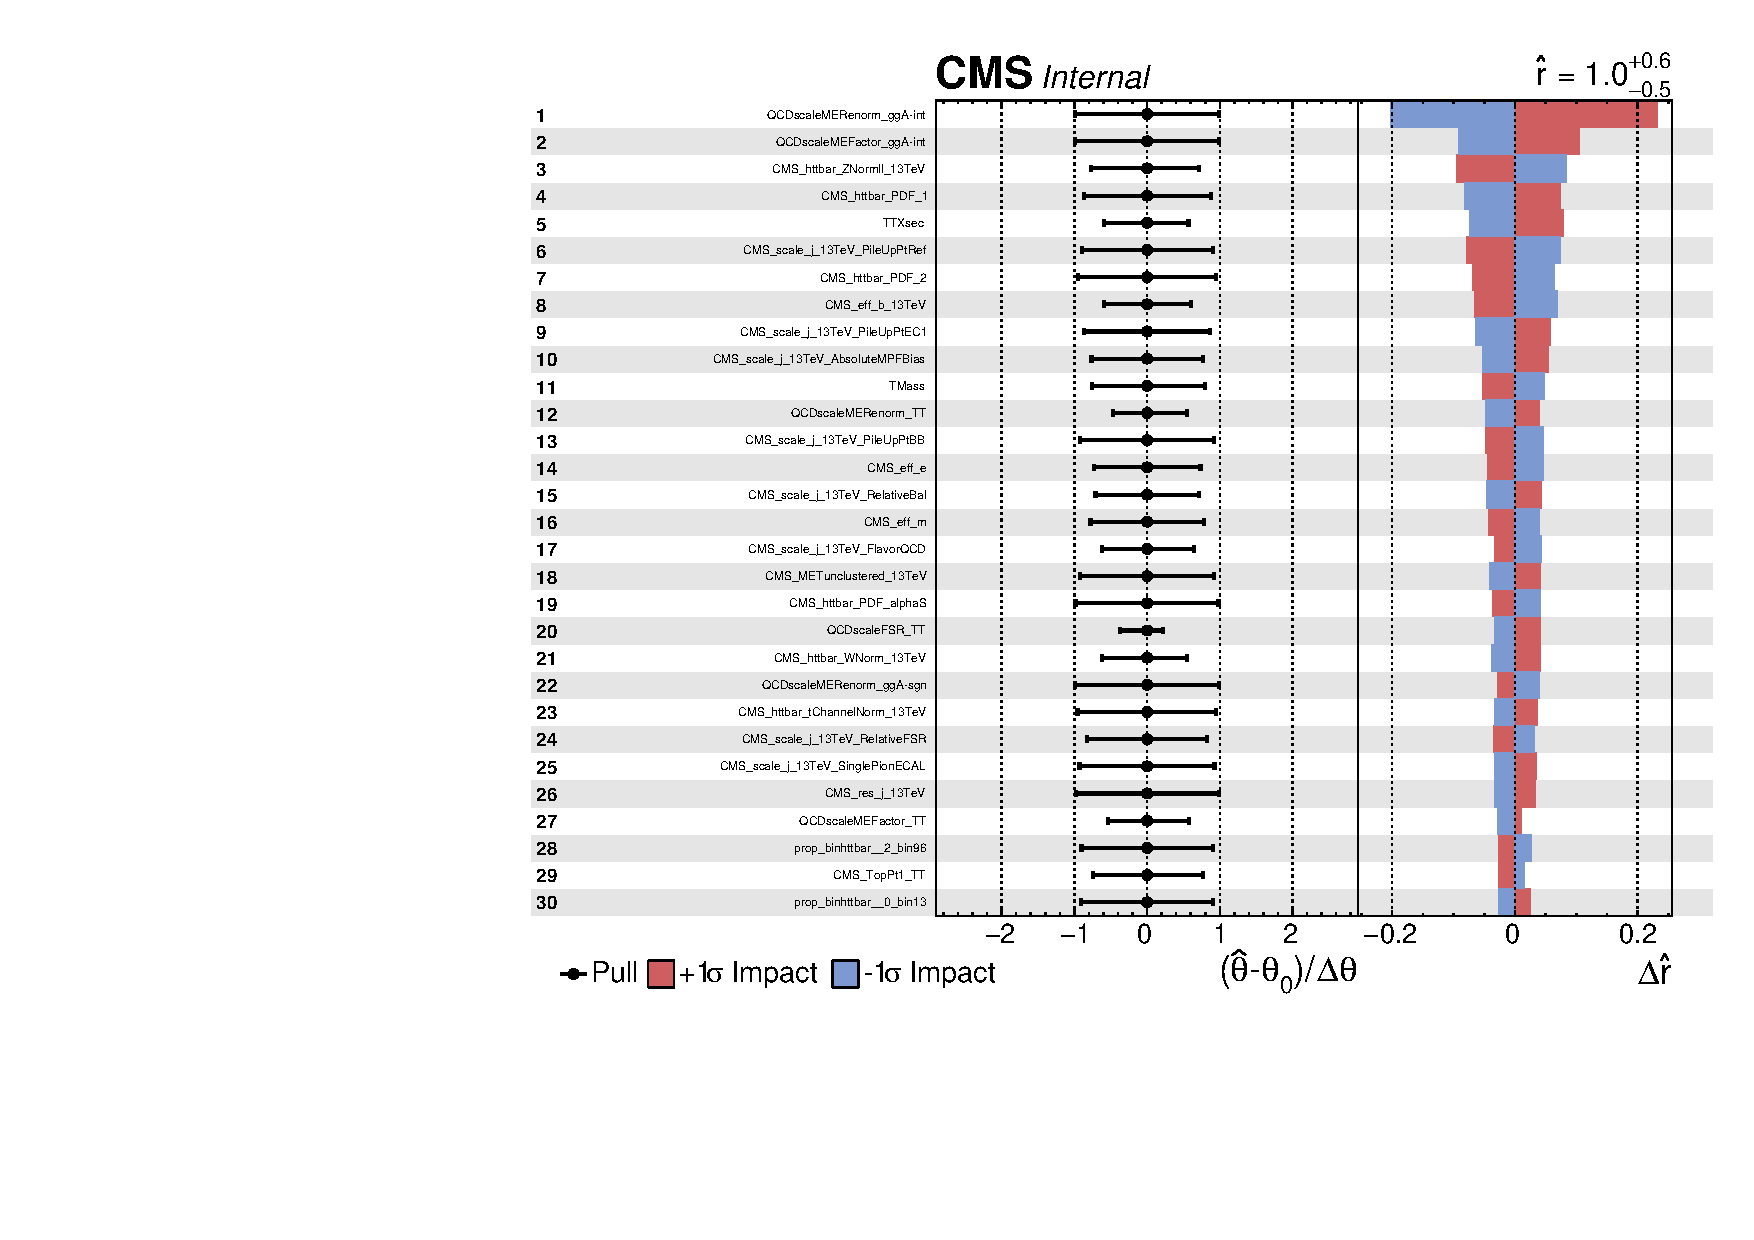
\includegraphics[width=0.85\textwidth,keepaspectratio=true]{fig/app5/impacts/impacts_600.pdf}
\caption{Impacts of systematic uncertainties on obtained coupling strength modifier for a 600\,GeV pseudoscalar with a relative width of 10\%. The impacts are shown for the Asimov dataset with a coupling strength modifier corresponding to the central expected limit. The right-hand side of the plot shows the relative variation of the obtained coupling strength under variations of the considered nuisance parameter within $\pm 1$ s.d.\ of its post-fit uncertainty (the so-called impact). The 30 uncertainties with the largest impact are shown. In addition, the post-fit value of the nuisance parameter and its uncertainty is shown on the left-hand side.}
\label{fig:iimpacts_m600}
\end{figure}

\begin{figure}[!Hhtb]
\centering
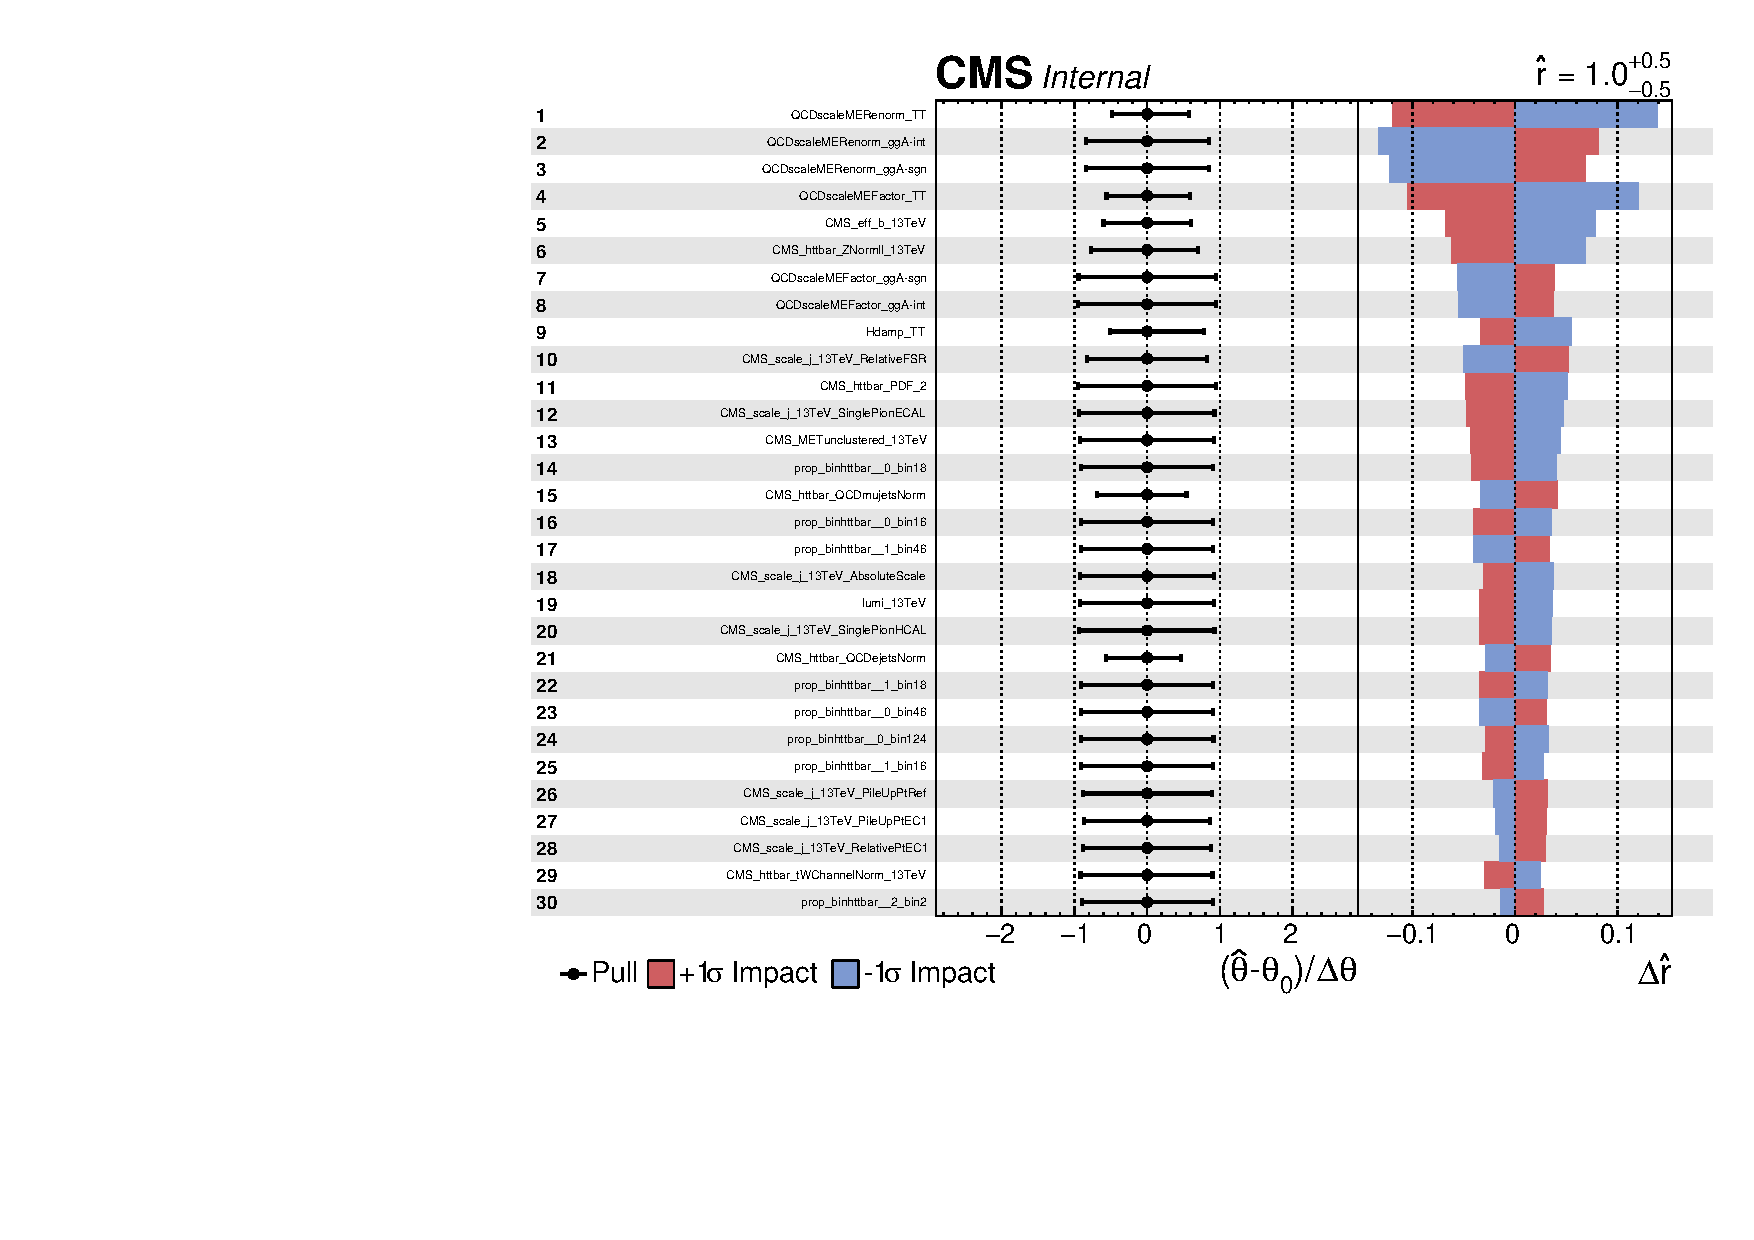
\includegraphics[width=0.85\textwidth,keepaspectratio=true]{fig/app5/impacts/impacts_750.pdf}
\caption{Impacts of systematic uncertainties on obtained coupling strength modifier for a 750\,GeV pseudoscalar with a relative width of 10\%. The impacts are shown for the Asimov dataset with a coupling strength modifier corresponding to the central expected limit. The right-hand side of the plot shows the relative variation of the obtained coupling strength under variations of the considered nuisance parameter within $\pm 1$ s.d.\ of its post-fit uncertainty (the so-called impact). The 30 uncertainties with the largest impact are shown. In addition, the post-fit value of the nuisance parameter and its uncertainty is shown on the left-hand side.}
\label{fig:impacts_m750}
\end{figure}


\begin{figure}[!Hhtb]
\centering
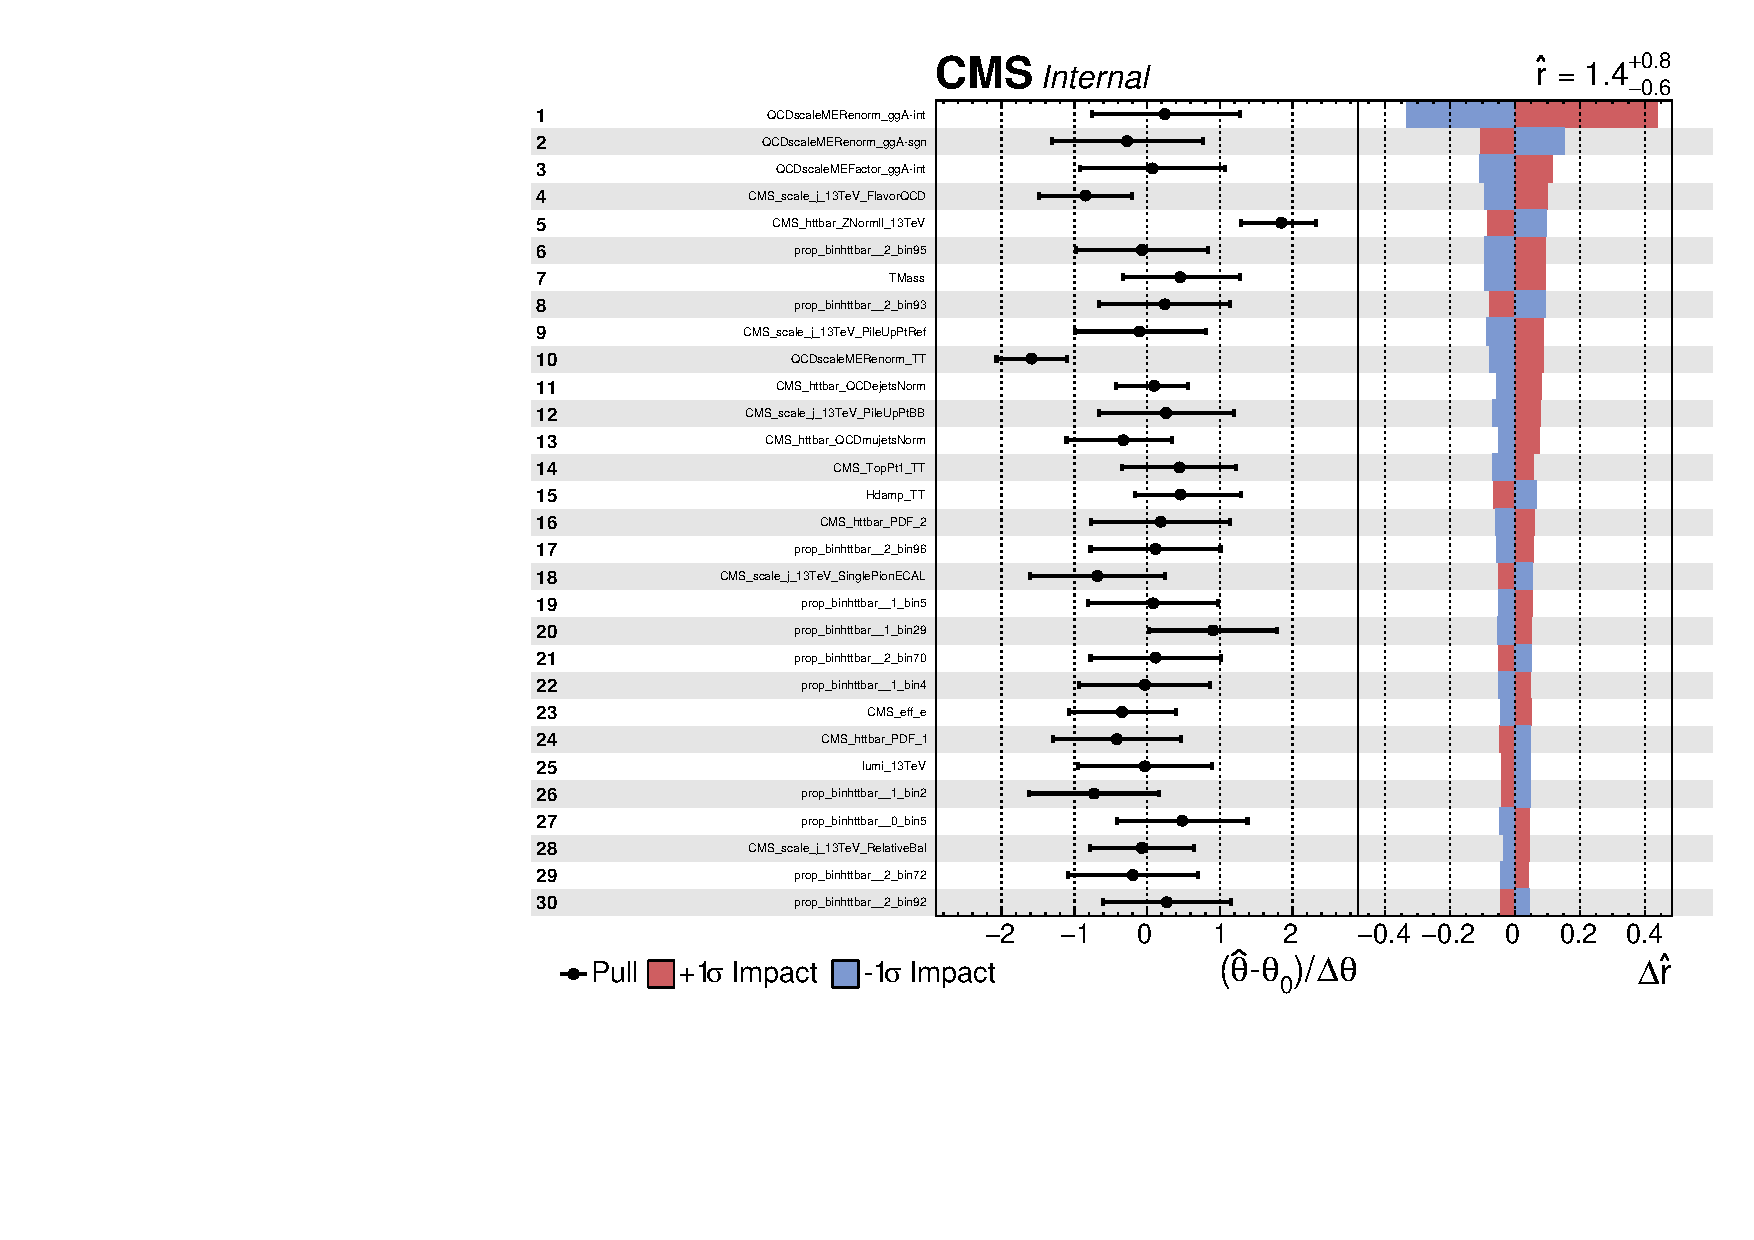
\includegraphics[width=0.85\textwidth,keepaspectratio=true]{fig/app5/impacts/impacts_400_obs.pdf}
\caption{Impacts of systematic uncertainties on obtained coupling strength modifier for a 400\,GeV pseudoscalar with a relative width of 2.5\%. The impacts are shown for the observed data with a coupling strength modifier corresponding to the central expected limit. The right-hand side of the plot shows the relative variation of the obtained coupling strength under variations of the considered nuisance parameter within $\pm 1$ s.d.\ of its post-fit uncertainty (the so-called impact). The 30 uncertainties with the largest impact are shown. In addition, the post-fit value of the nuisance parameter and its uncertainty is shown on the left-hand side.}
\label{fig:impacts_obs_m400}
\end{figure}

\begin{figure}[!Hhtb]
\centering
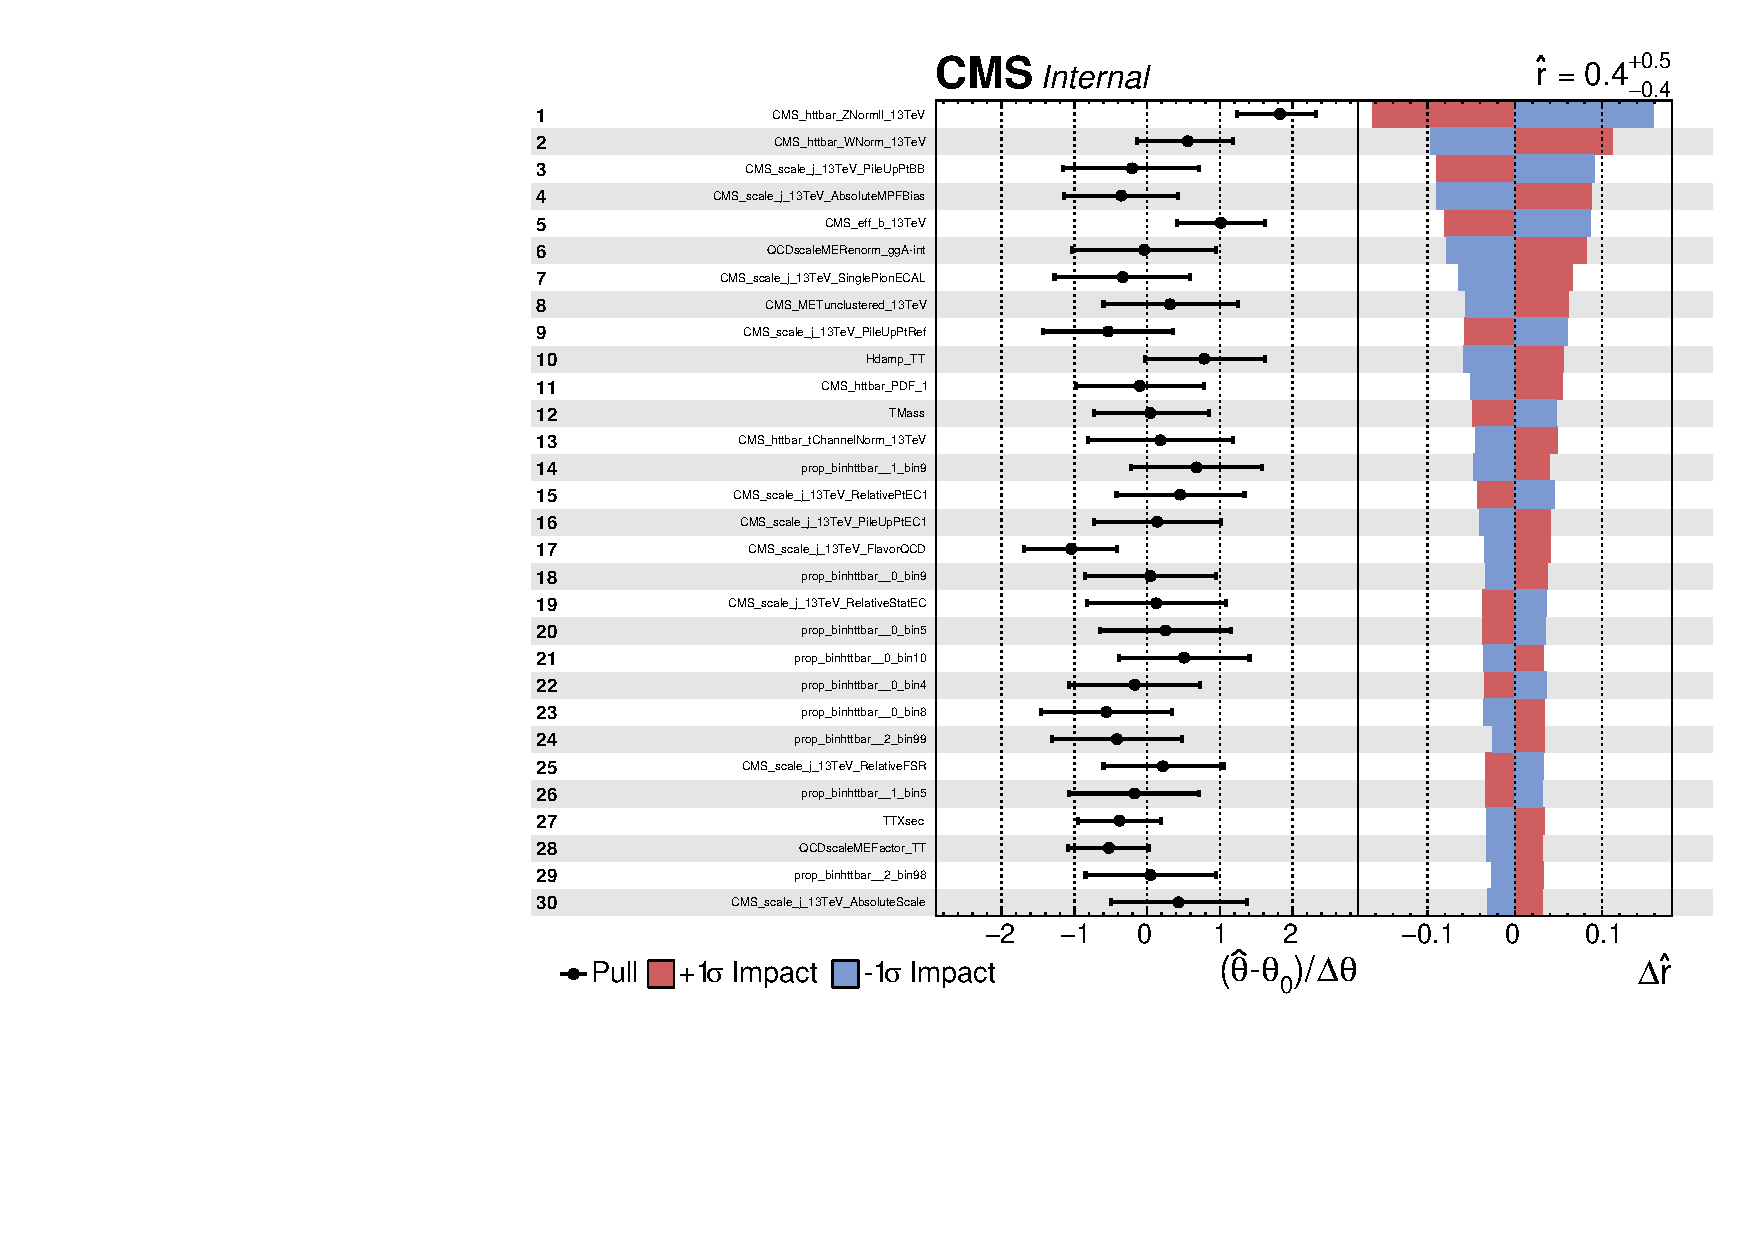
\includegraphics[width=0.85\textwidth,keepaspectratio=true]{fig/app5/impacts/impacts_500_obs.pdf}
\caption{Impacts of systematic uncertainties on obtained coupling strength modifier for a 500\,GeV pseudoscalar with a relative width of 5\%. The impacts are shown for the observed data with a coupling strength modifier corresponding to the central expected limit. The right-hand side of the plot shows the relative variation of the obtained coupling strength under variations of the considered nuisance parameter within $\pm 1$ s.d.\ of its post-fit uncertainty (the so-called impact). The 30 uncertainties with the largest impact are shown. In addition, the post-fit value of the nuisance parameter and its uncertainty is shown on the left-hand side.}
\label{fig:impacts_obs_m500}
\end{figure}

\begin{figure}[!Hhtb]
\centering
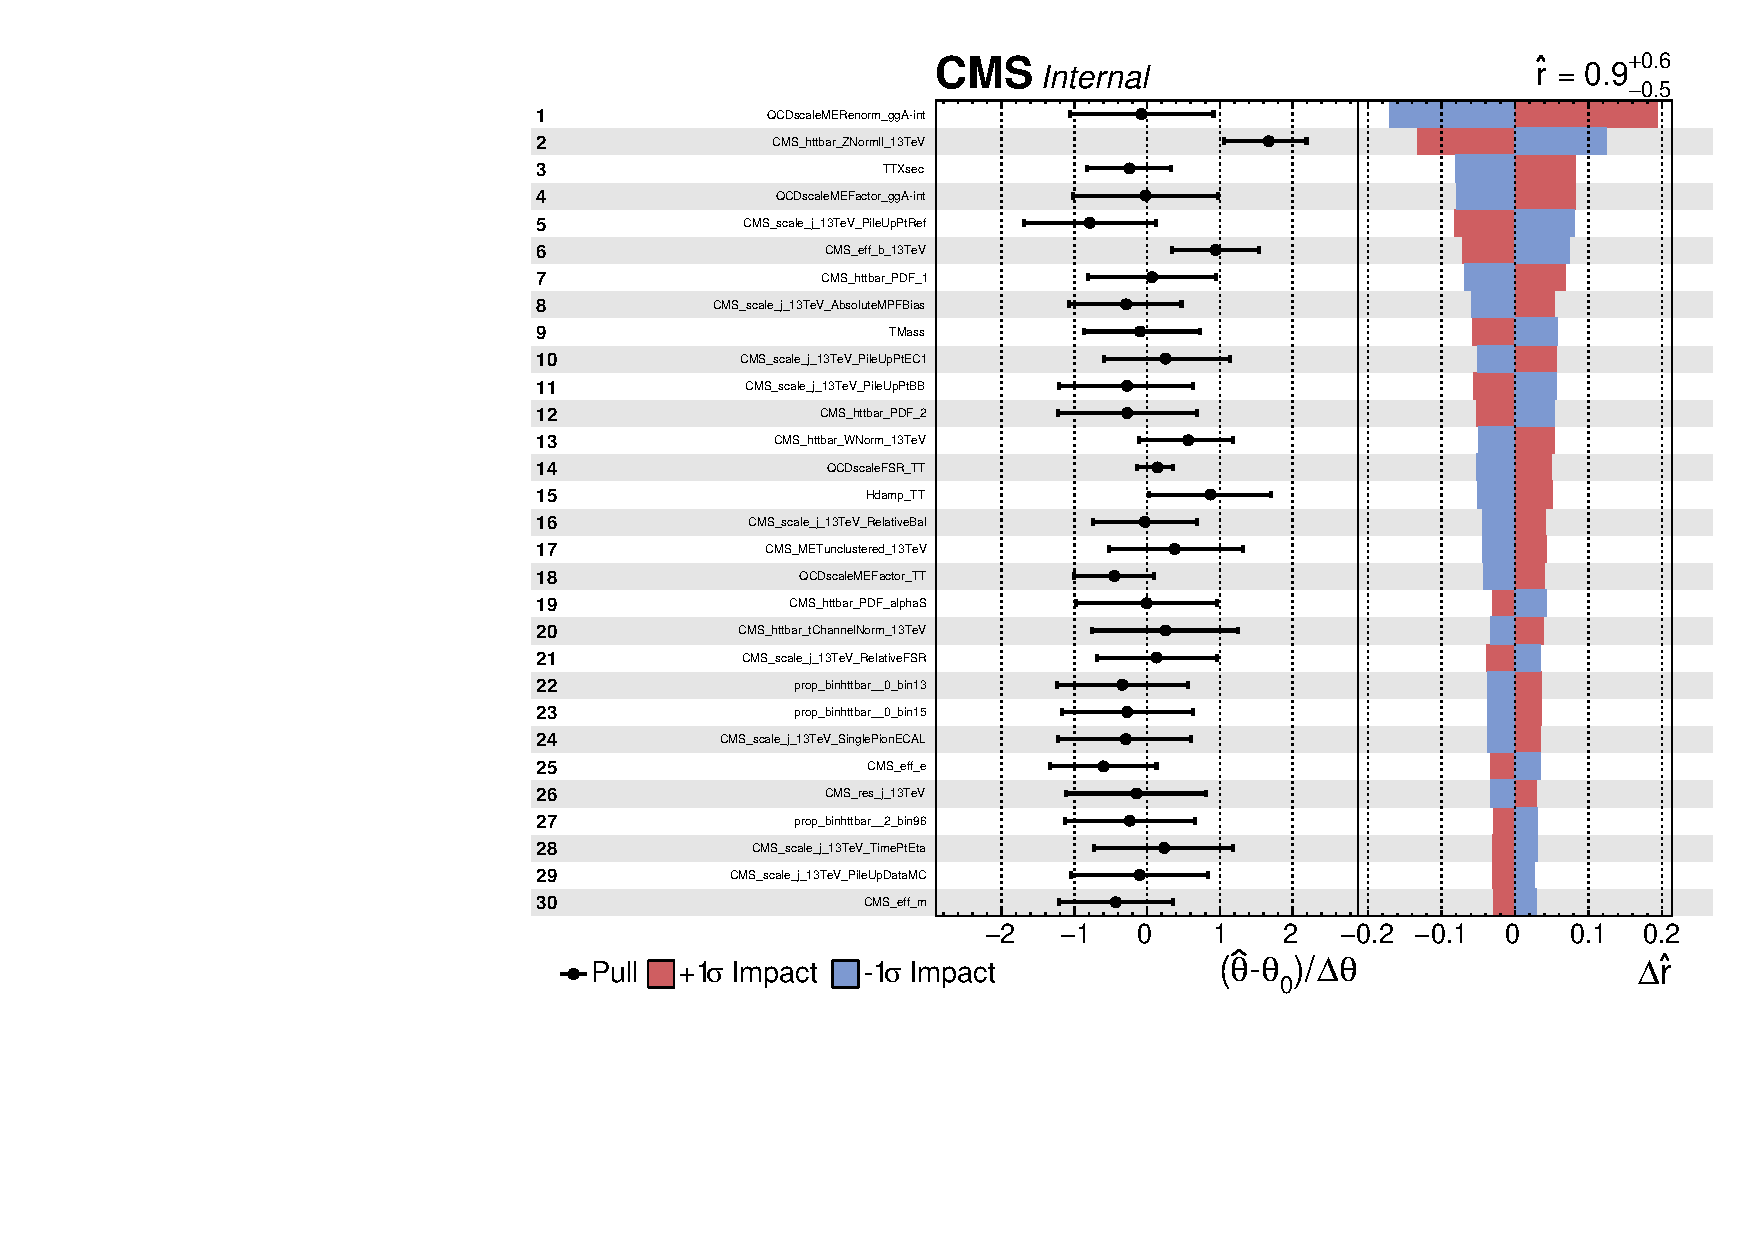
\includegraphics[width=0.85\textwidth,keepaspectratio=true]{fig/app5/impacts/impacts_600_obs.pdf}
\caption{Impacts of systematic uncertainties on obtained coupling strength modifier for a 600\,GeV pseudoscalar with a relative width of 10\%. The impacts are shown for the observed data with a coupling strength modifier corresponding to the central expected limit. The right-hand side of the plot shows the relative variation of the obtained coupling strength under variations of the considered nuisance parameter within $\pm 1$ s.d.\ of its post-fit uncertainty (the so-called impact). The 30 uncertainties with the largest impact are shown. In addition, the post-fit value of the nuisance parameter and its uncertainty is shown on the left-hand side.}
\label{fig:iimpacts_obs_m600}
\end{figure}

\begin{figure}[!Hhtb]
\centering
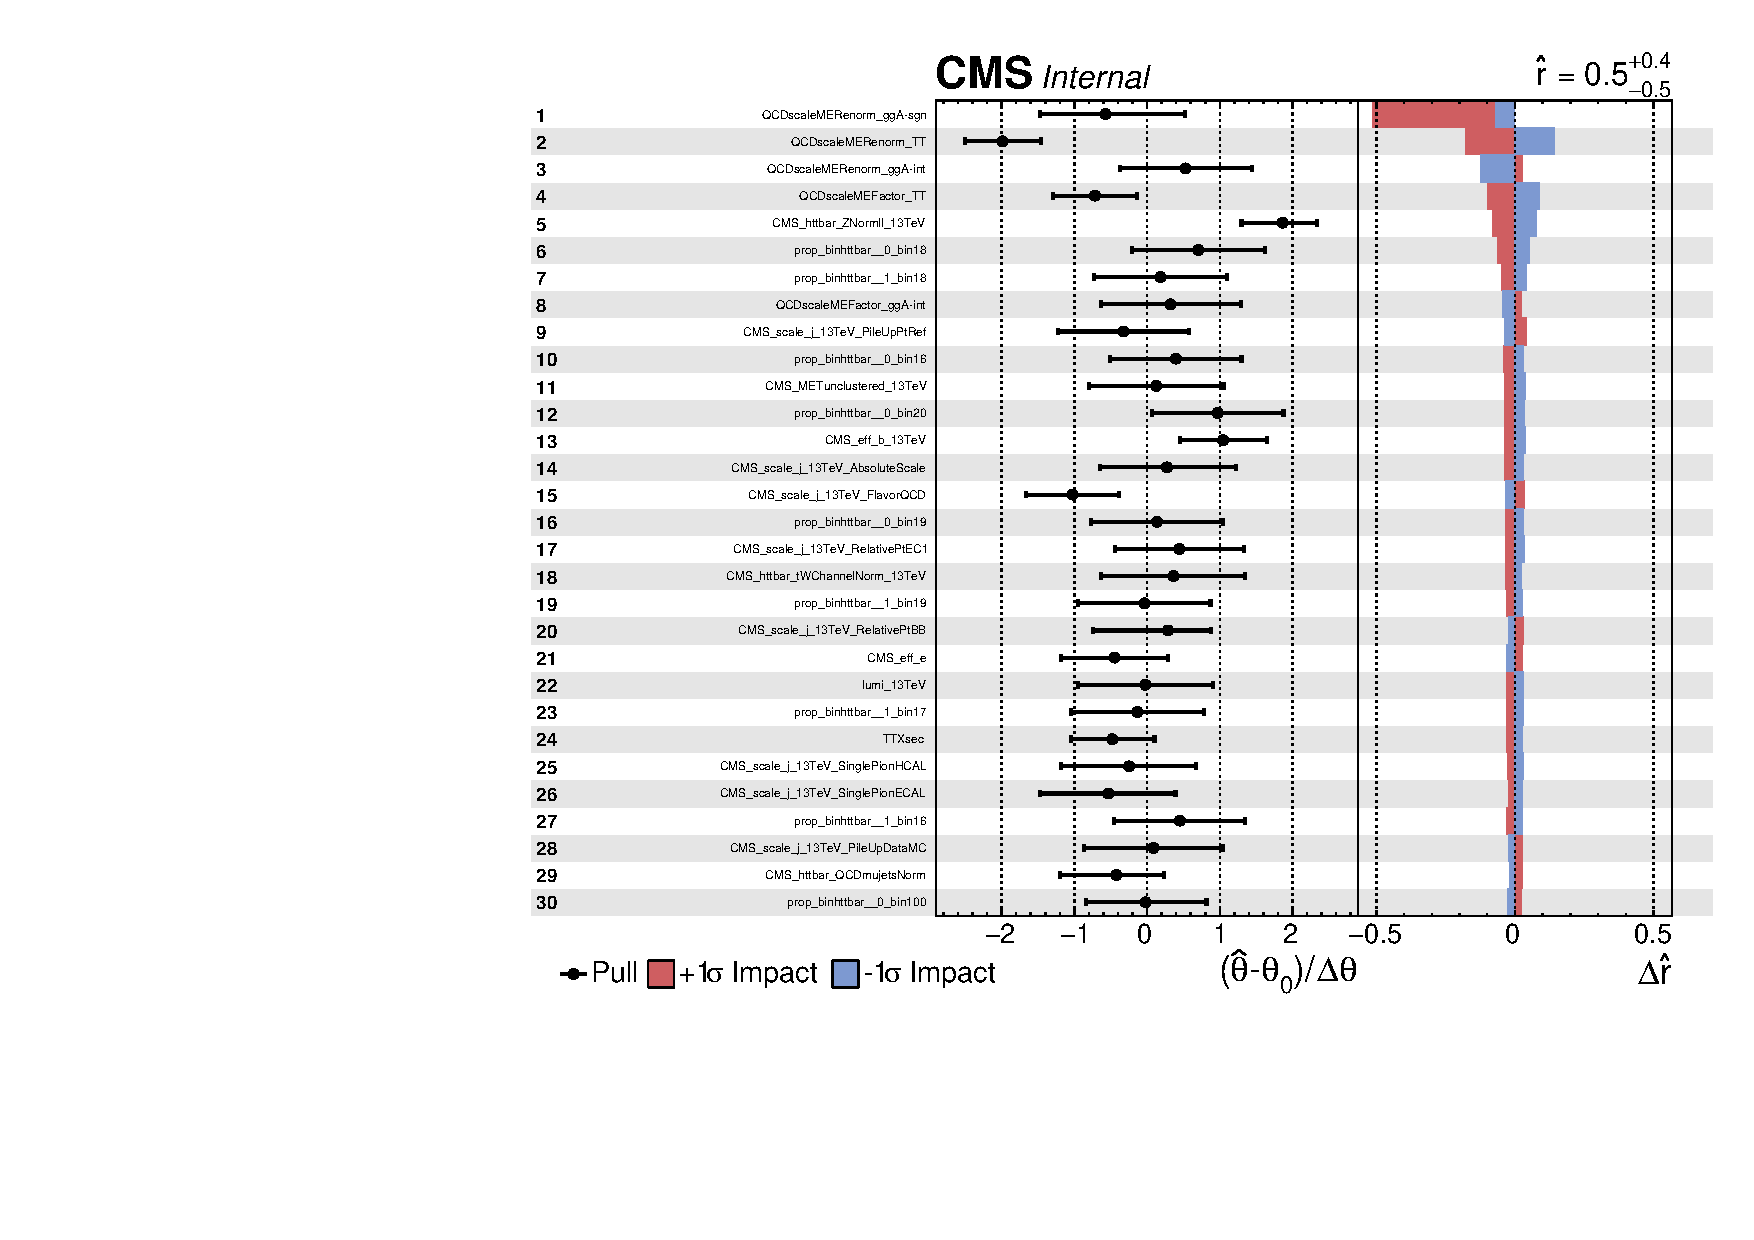
\includegraphics[width=0.85\textwidth,keepaspectratio=true]{fig/app5/impacts/impacts_750_obs.pdf}
\caption{Impacts of systematic uncertainties on obtained coupling strength modifier for a 750\,GeV pseudoscalar with a relative width of 10\%. The impacts are shown for the observed data with a coupling strength modifier corresponding to the central expected limit. The right-hand side of the plot shows the relative variation of the obtained coupling strength under variations of the considered nuisance parameter within $\pm 1$ s.d.\ of its post-fit uncertainty (the so-called impact). The 30 uncertainties with the largest impact are shown. In addition, the post-fit value of the nuisance parameter and its uncertainty is shown on the left-hand side.}
\label{fig:impacts_obs_m750}
\end{figure}


Figures~\ref{fig:impacts_m400}-\ref{fig:impacts_m750} (expected) and Figs.\ \ref{fig:impacts_obs_m400}-\ref{fig:impacts_obs_m750} (observed) give a summary of the 30 most important systematic uncertainties for 4 different scenarios that range from low to high mass, with the widths near the exclusion in the hMSSM scenario, and the value of the coupling modifier adjusted to the central expected limit.
Like for the fits carried out to obtain the limits, the coupling modifier is fixed in the fit, and only the signal strength modifier is kept floating.
Impacts are hence calculated on the signal strength modifier, with an injected signal strength of unity for the expected impacts.
The left parts of the figures contain the post-fit values of these nuisance parameters and their post-fit constraint.
The right parts of the figures show the impact of each such uncertainty on the observed signal strength, which can also be understood as the contribution of each systematic uncertainty to the overall uncertainty.
It can be noted that, in all cases, theory-related systematic uncertainties constitute the most important sources of systematic uncertainty, in particular also those related to the dominant $t\bar t$ background.
At lower mass, the uncertainty in the value of the top quark mass is more important, which can be understood from the $m_{t\bar t}$ distribution being sensitive because of threshold effects, whereas missing higher orders are more relevant at higher masses.

It can also be noted that some uncertainties are subject to significant constraints.
A few of the theoretical uncertainties pertaining to $t\bar t$ simulation are expected to be constrained.
For example, the variation of FSR in $t\bar t$ simulated events and other variations were found to be larger than the uncertainties also in dedicated $t\bar t$ studies~\cite{CMS-PAS-TOP-16-021}.
Similarly, it has been investigated previously that the $m_{t\bar t}$ distribution, in particular the turn-on region, is sensitive to the top quark mass~\cite{CMS_AN_2008_21}.
In terms of experimental uncertainties, we note that there are moderate to tight constraints on the variations from all sources of uncertainties in the jet energy corrections. 


\subsection{Groups}
\label{sec:group_unc}

\begin{figure}[!Hhtb]
\centering
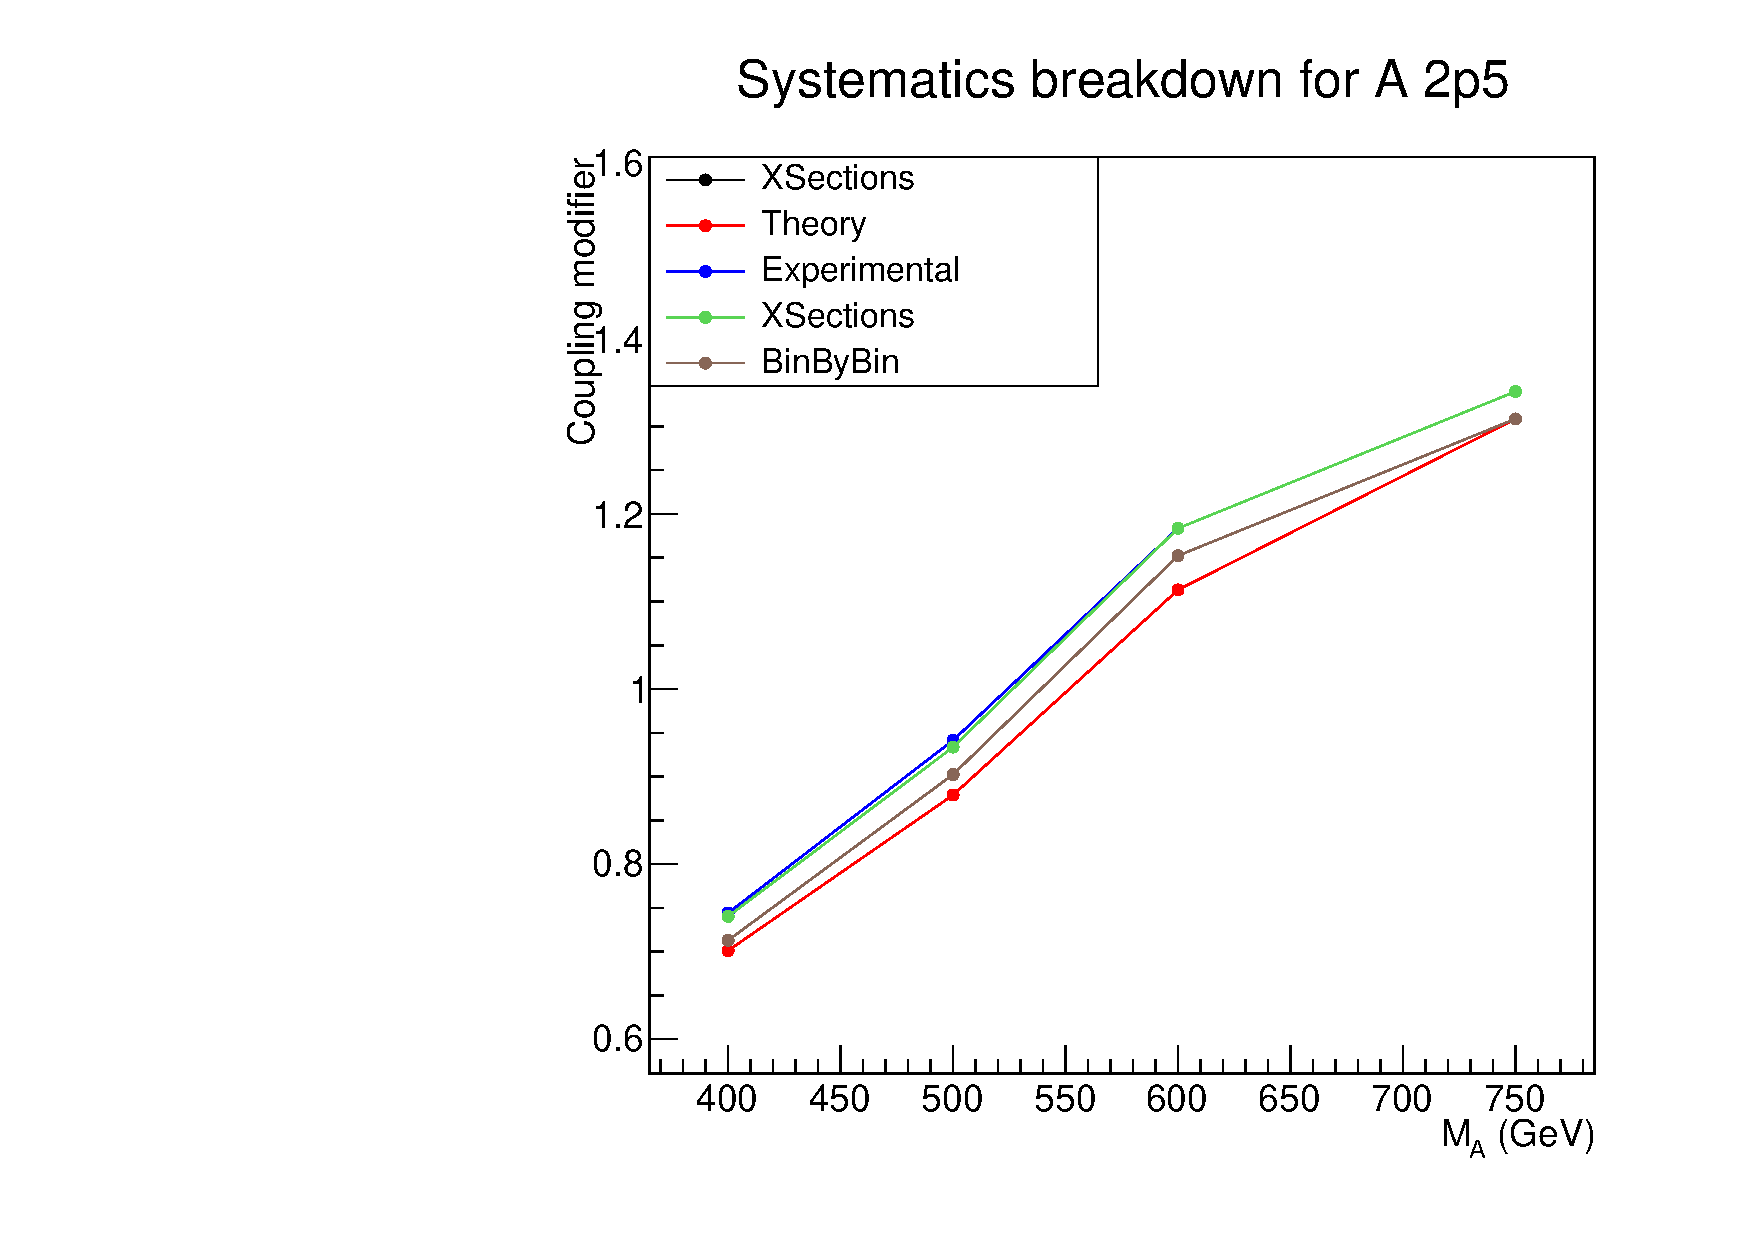
\includegraphics[width=0.35\textwidth,keepaspectratio=true]{fig/app5/breakdowns/generic_breakdown_A_2p5.pdf}
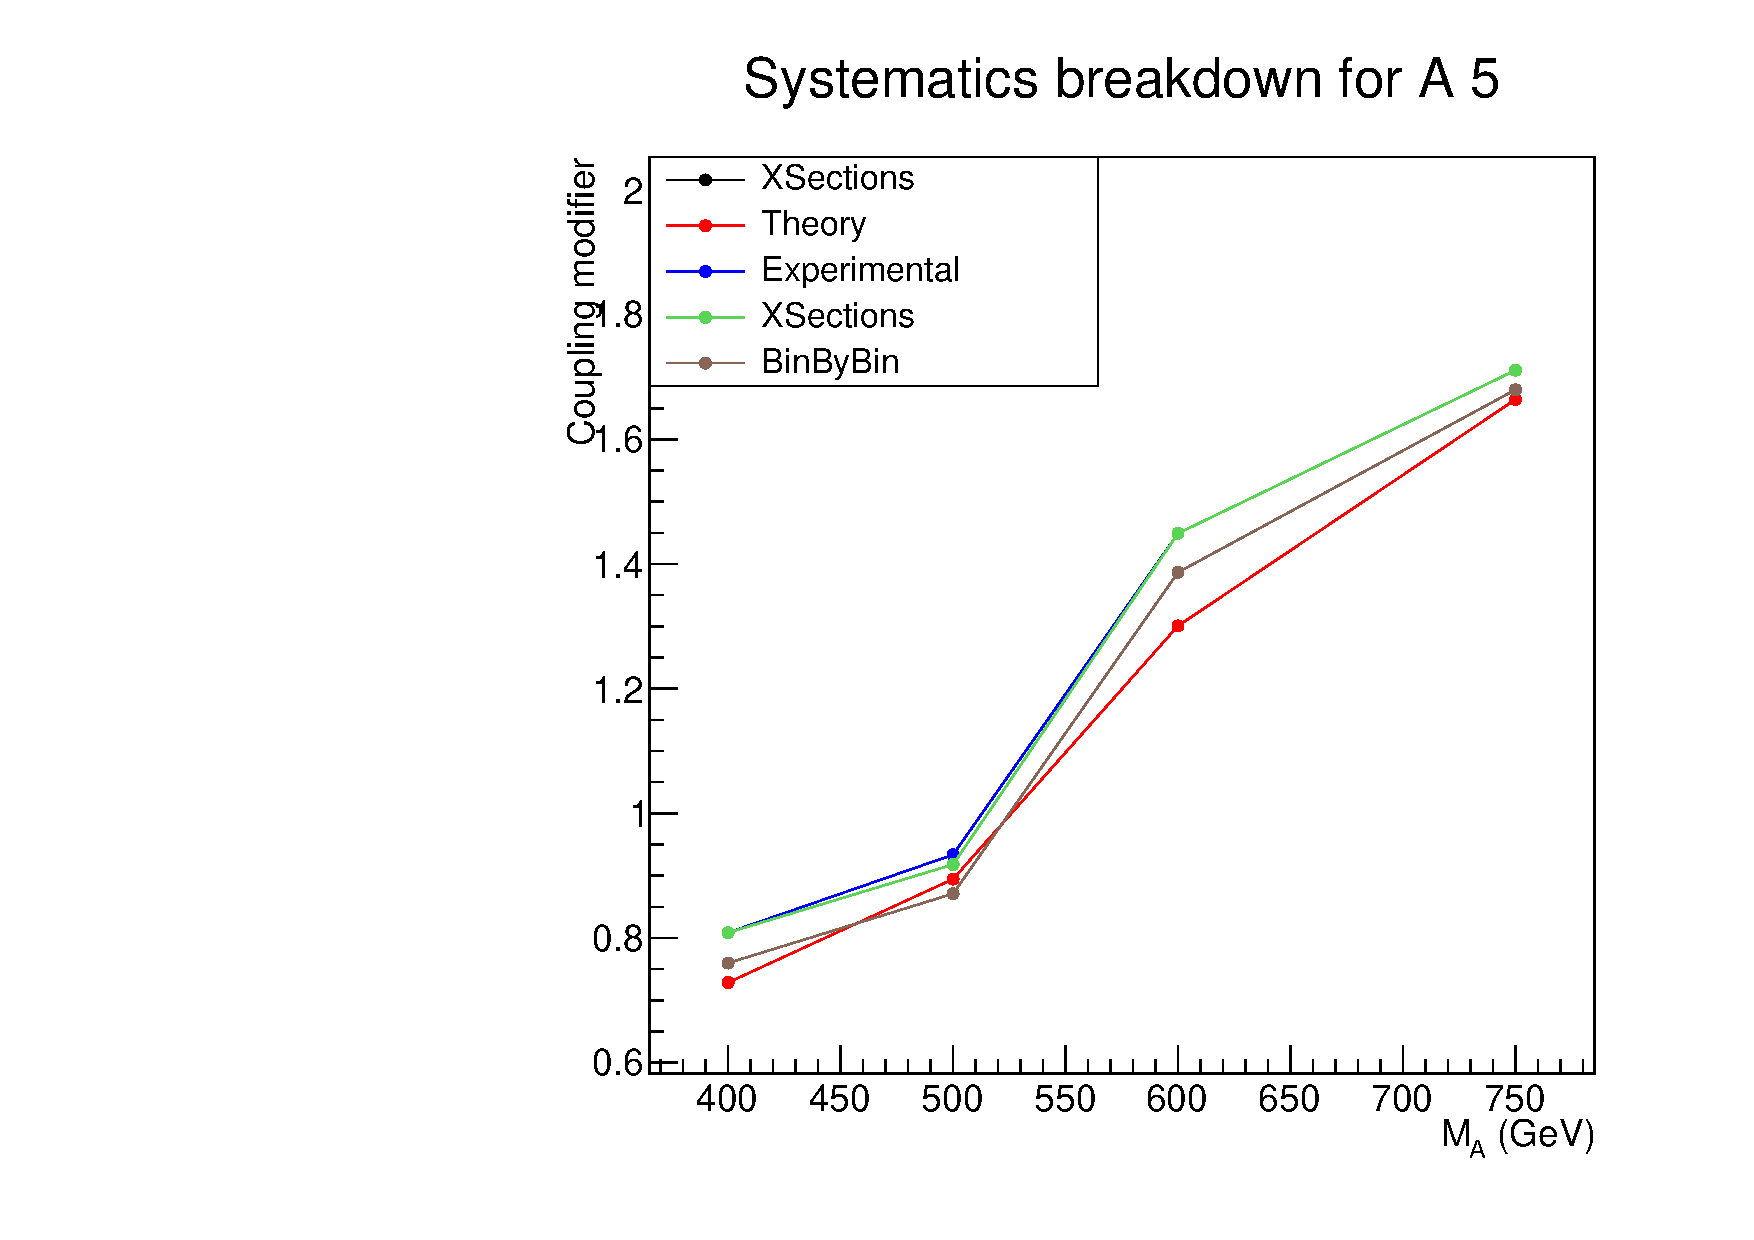
\includegraphics[width=0.35\textwidth,keepaspectratio=true]{fig/app5/breakdowns/generic_breakdown_A_5.pdf}
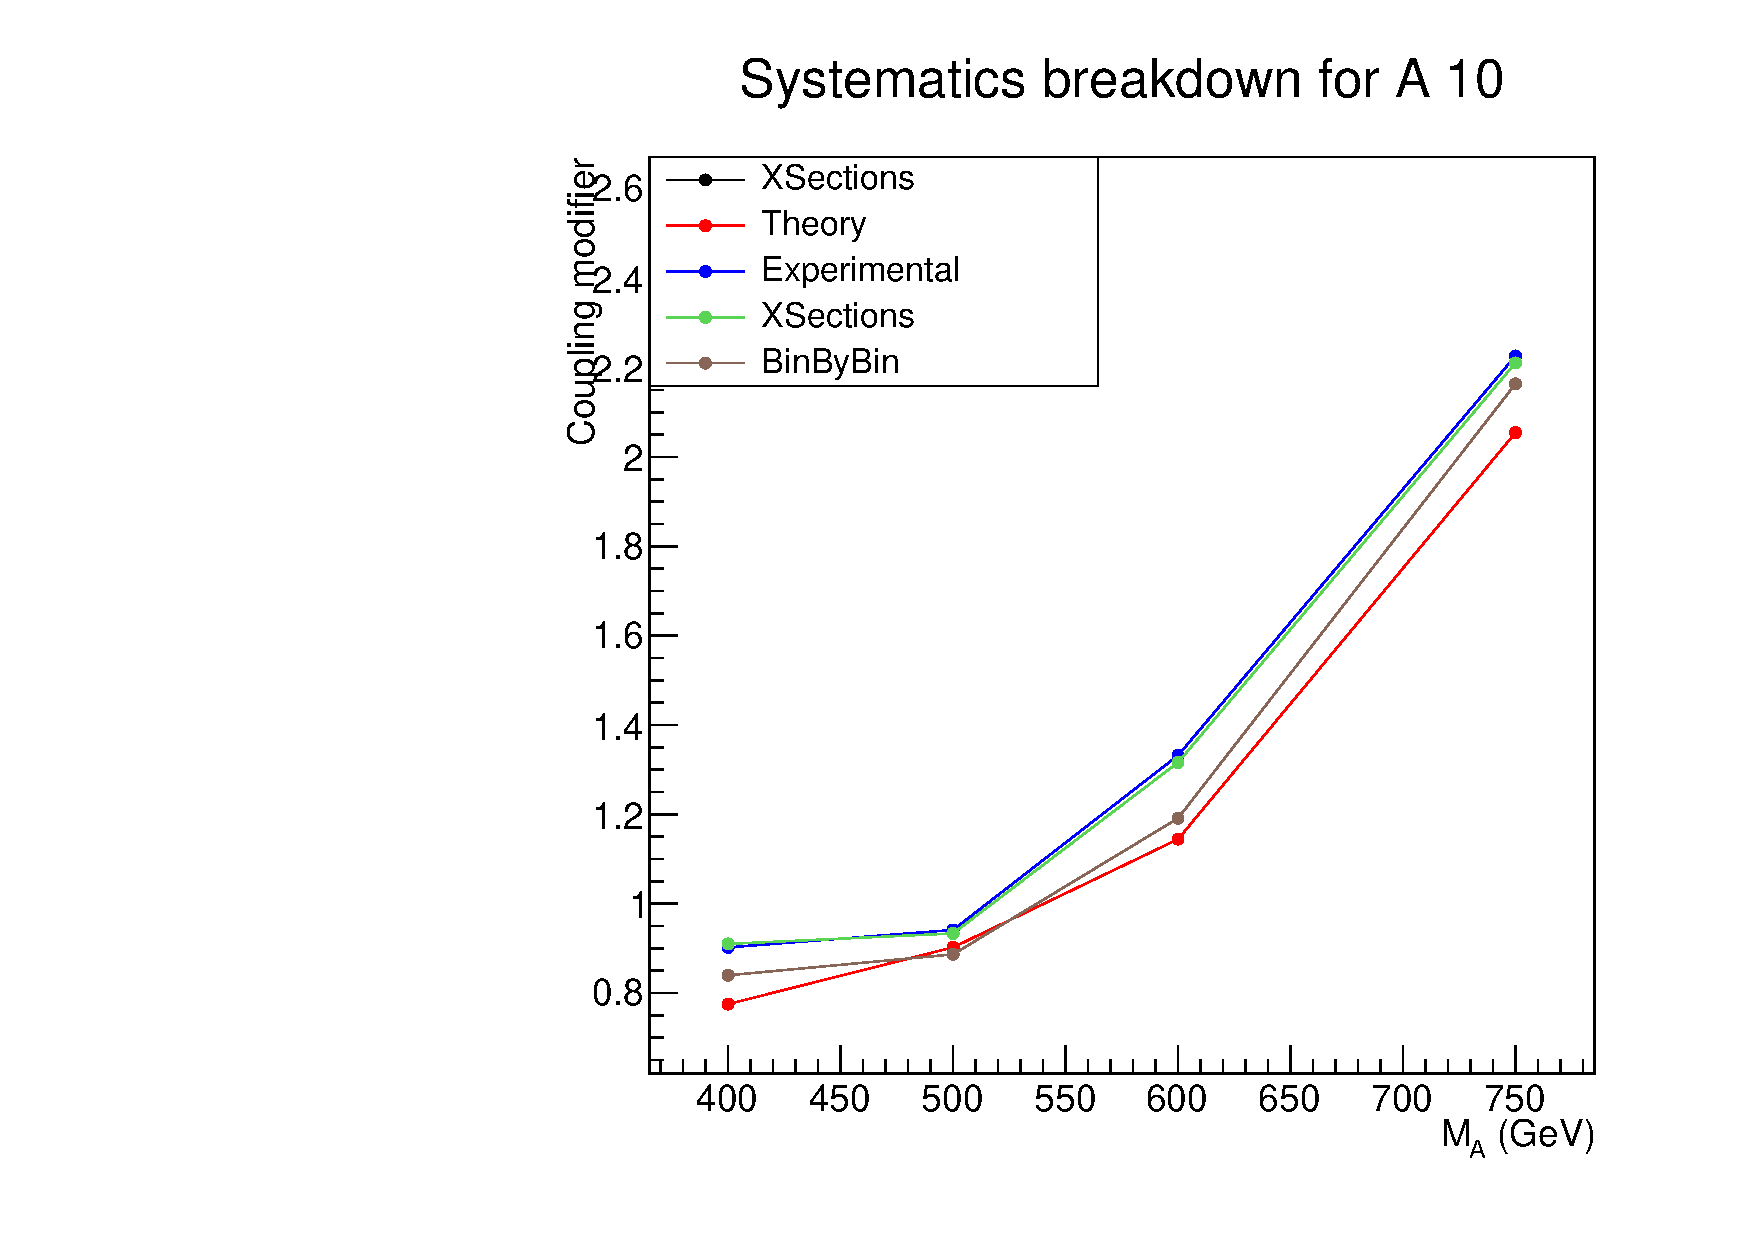
\includegraphics[width=0.35\textwidth,keepaspectratio=true]{fig/app5/breakdowns/generic_breakdown_A_10.pdf}
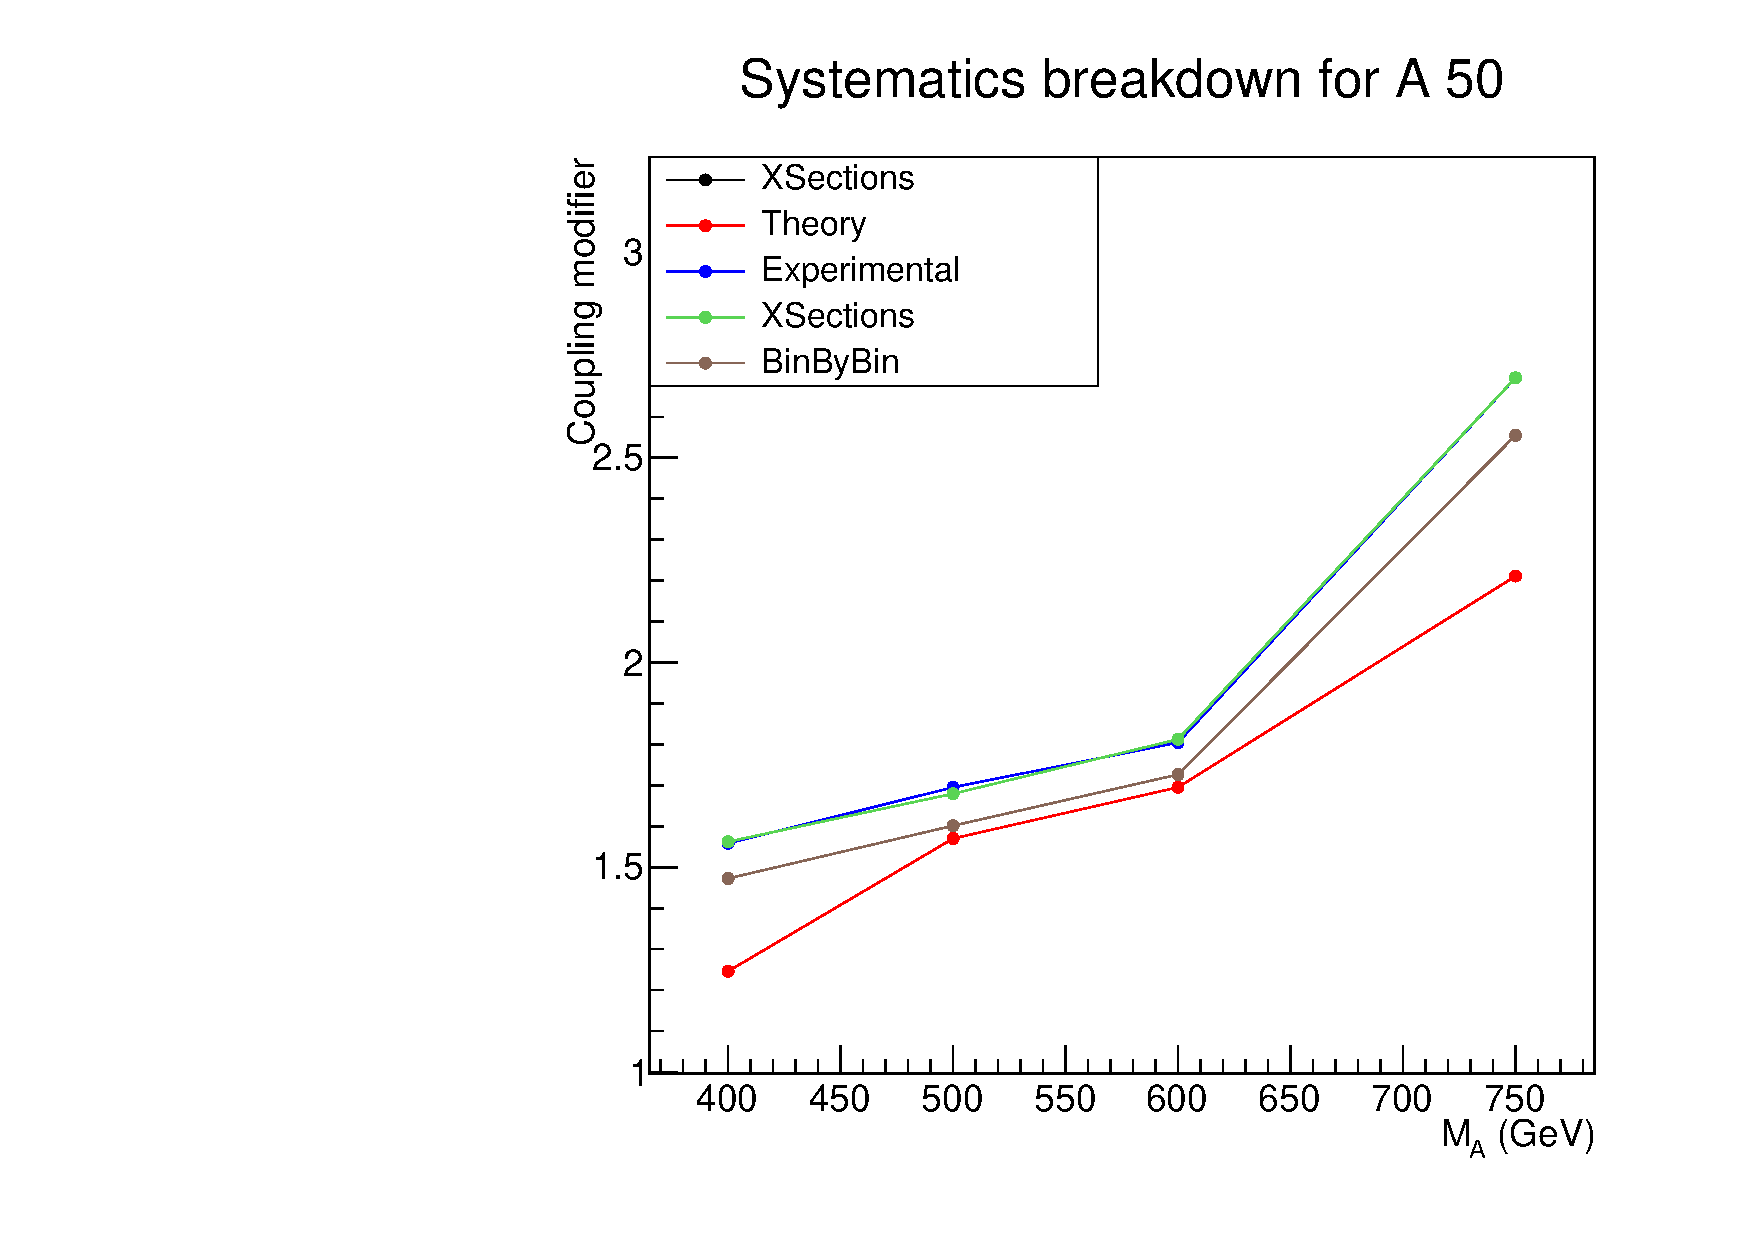
\includegraphics[width=0.35\textwidth,keepaspectratio=true]{fig/app5/breakdowns/generic_breakdown_A_50.pdf}
\caption{Expected upper limits on the coupling modifier with different groups of systematic uncertainties removed. The nominal limits are shown as the blue curve. The expected upper limits are shown for pseudoscalar signal as a function of mass for different values of the relative width, ranging from 2.5 to 50\%.}
\label{fig:breakdown_awidths}
\end{figure}
\begin{figure}[!Hhtb]
\centering
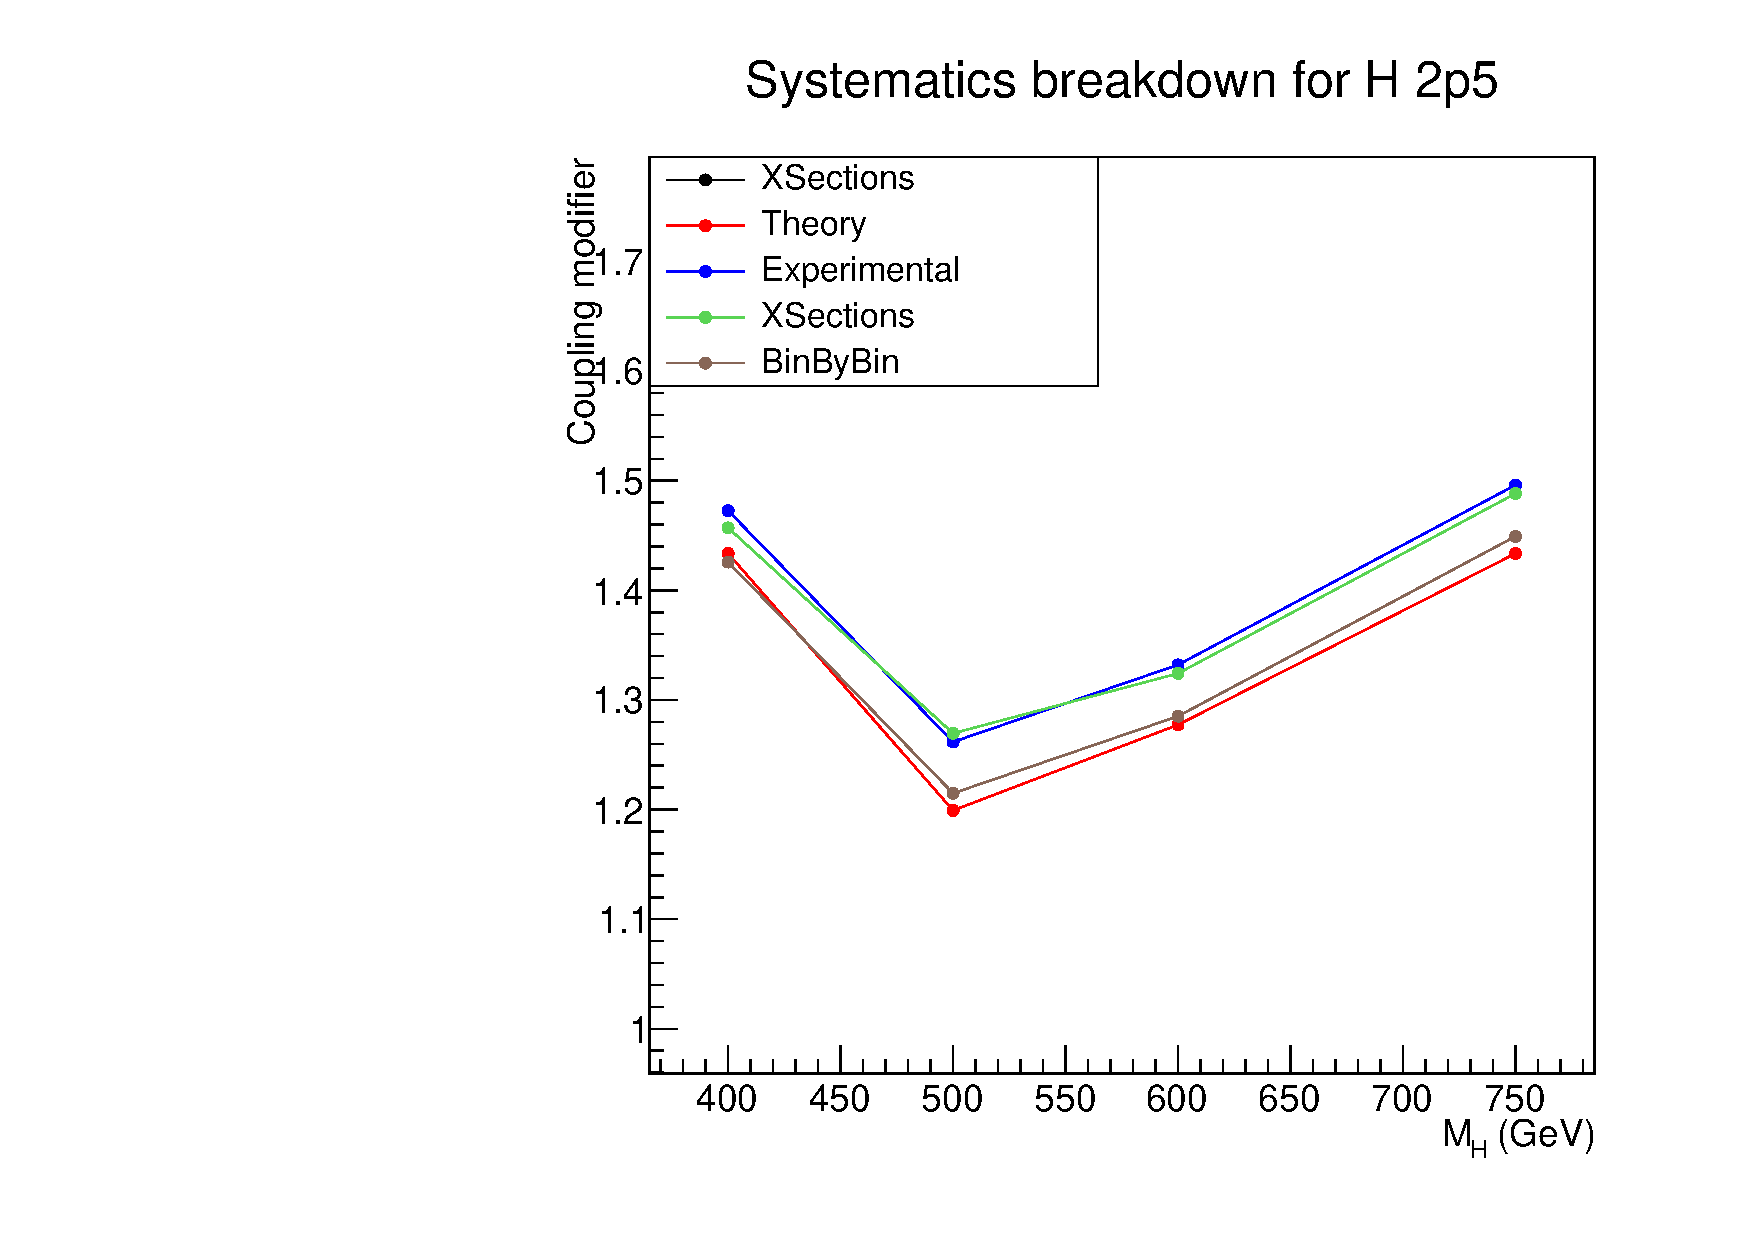
\includegraphics[width=0.35\textwidth,keepaspectratio=true]{fig/app5/breakdowns/generic_breakdown_H_2p5.pdf}
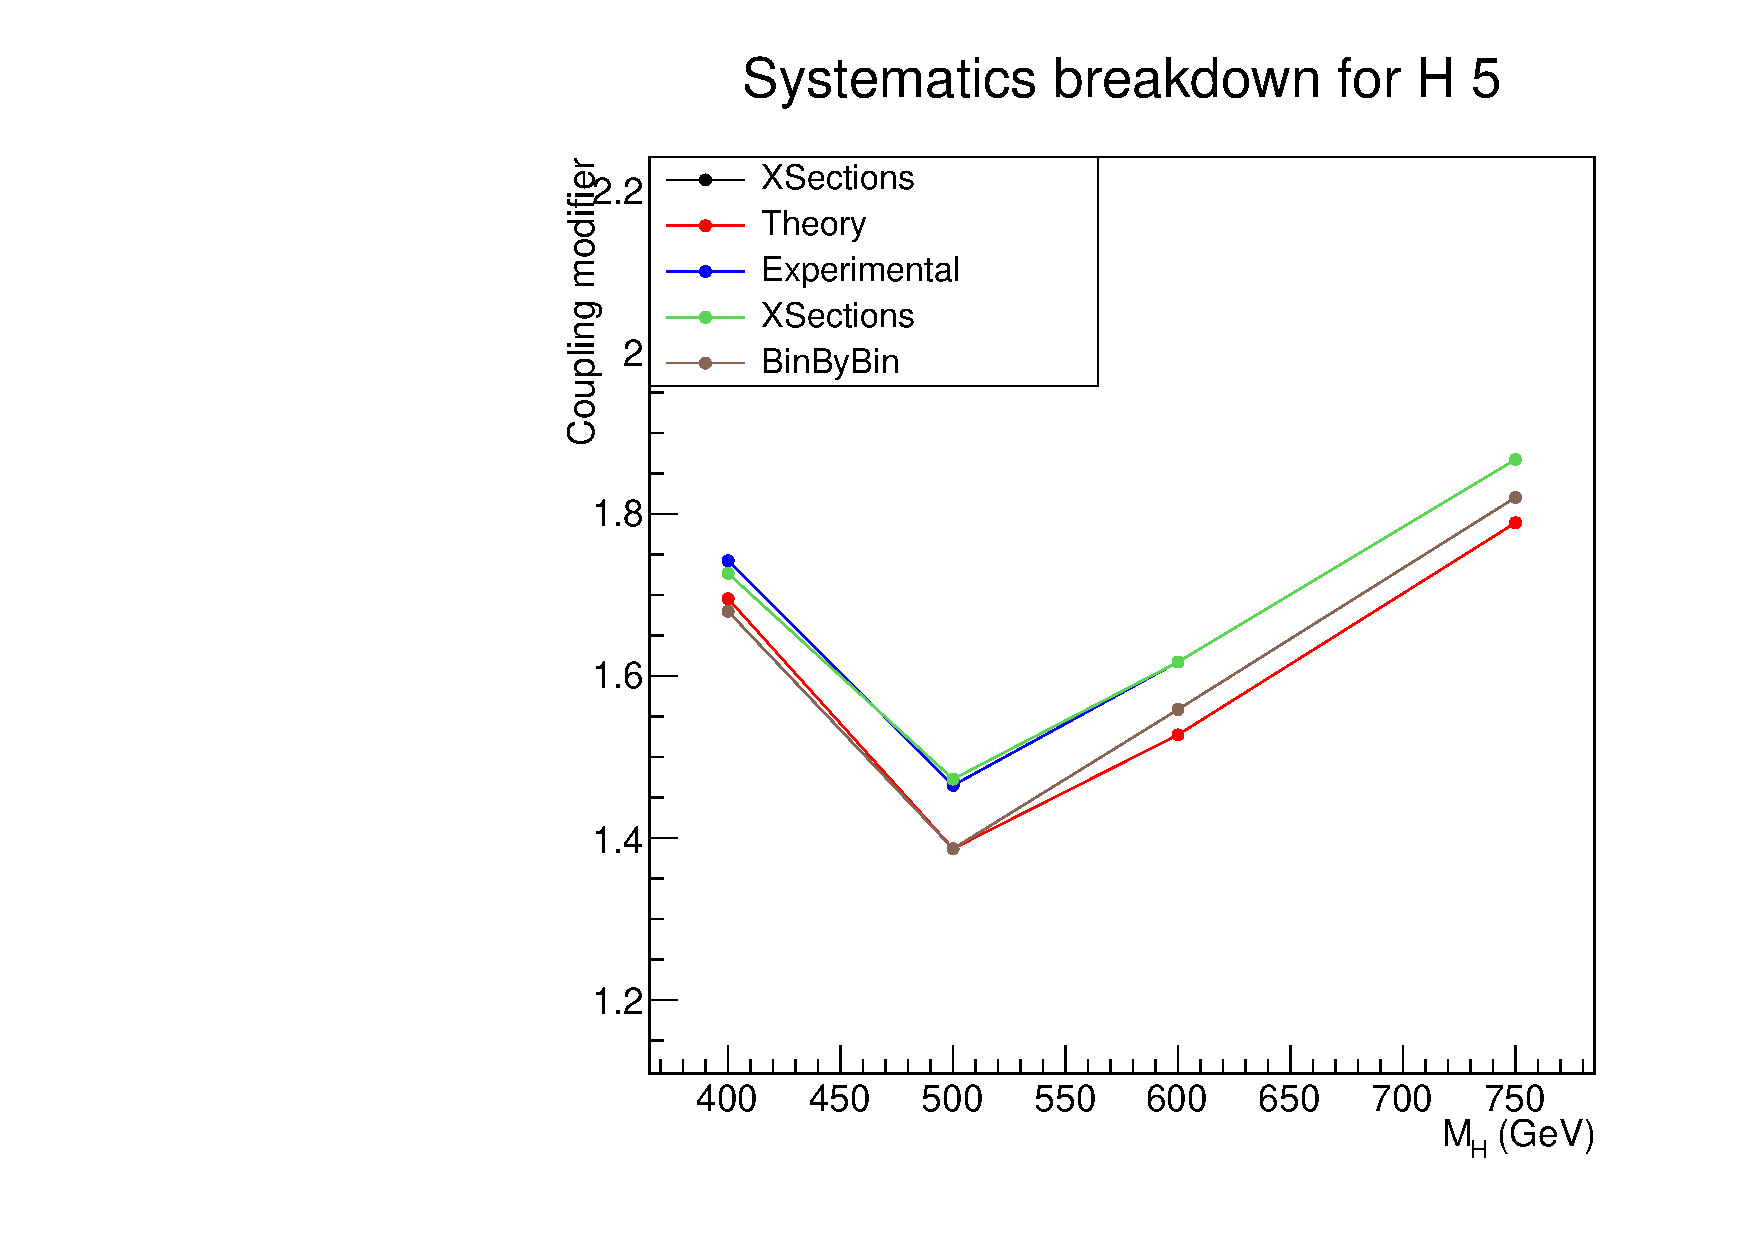
\includegraphics[width=0.35\textwidth,keepaspectratio=true]{fig/app5/breakdowns/generic_breakdown_H_5.pdf}
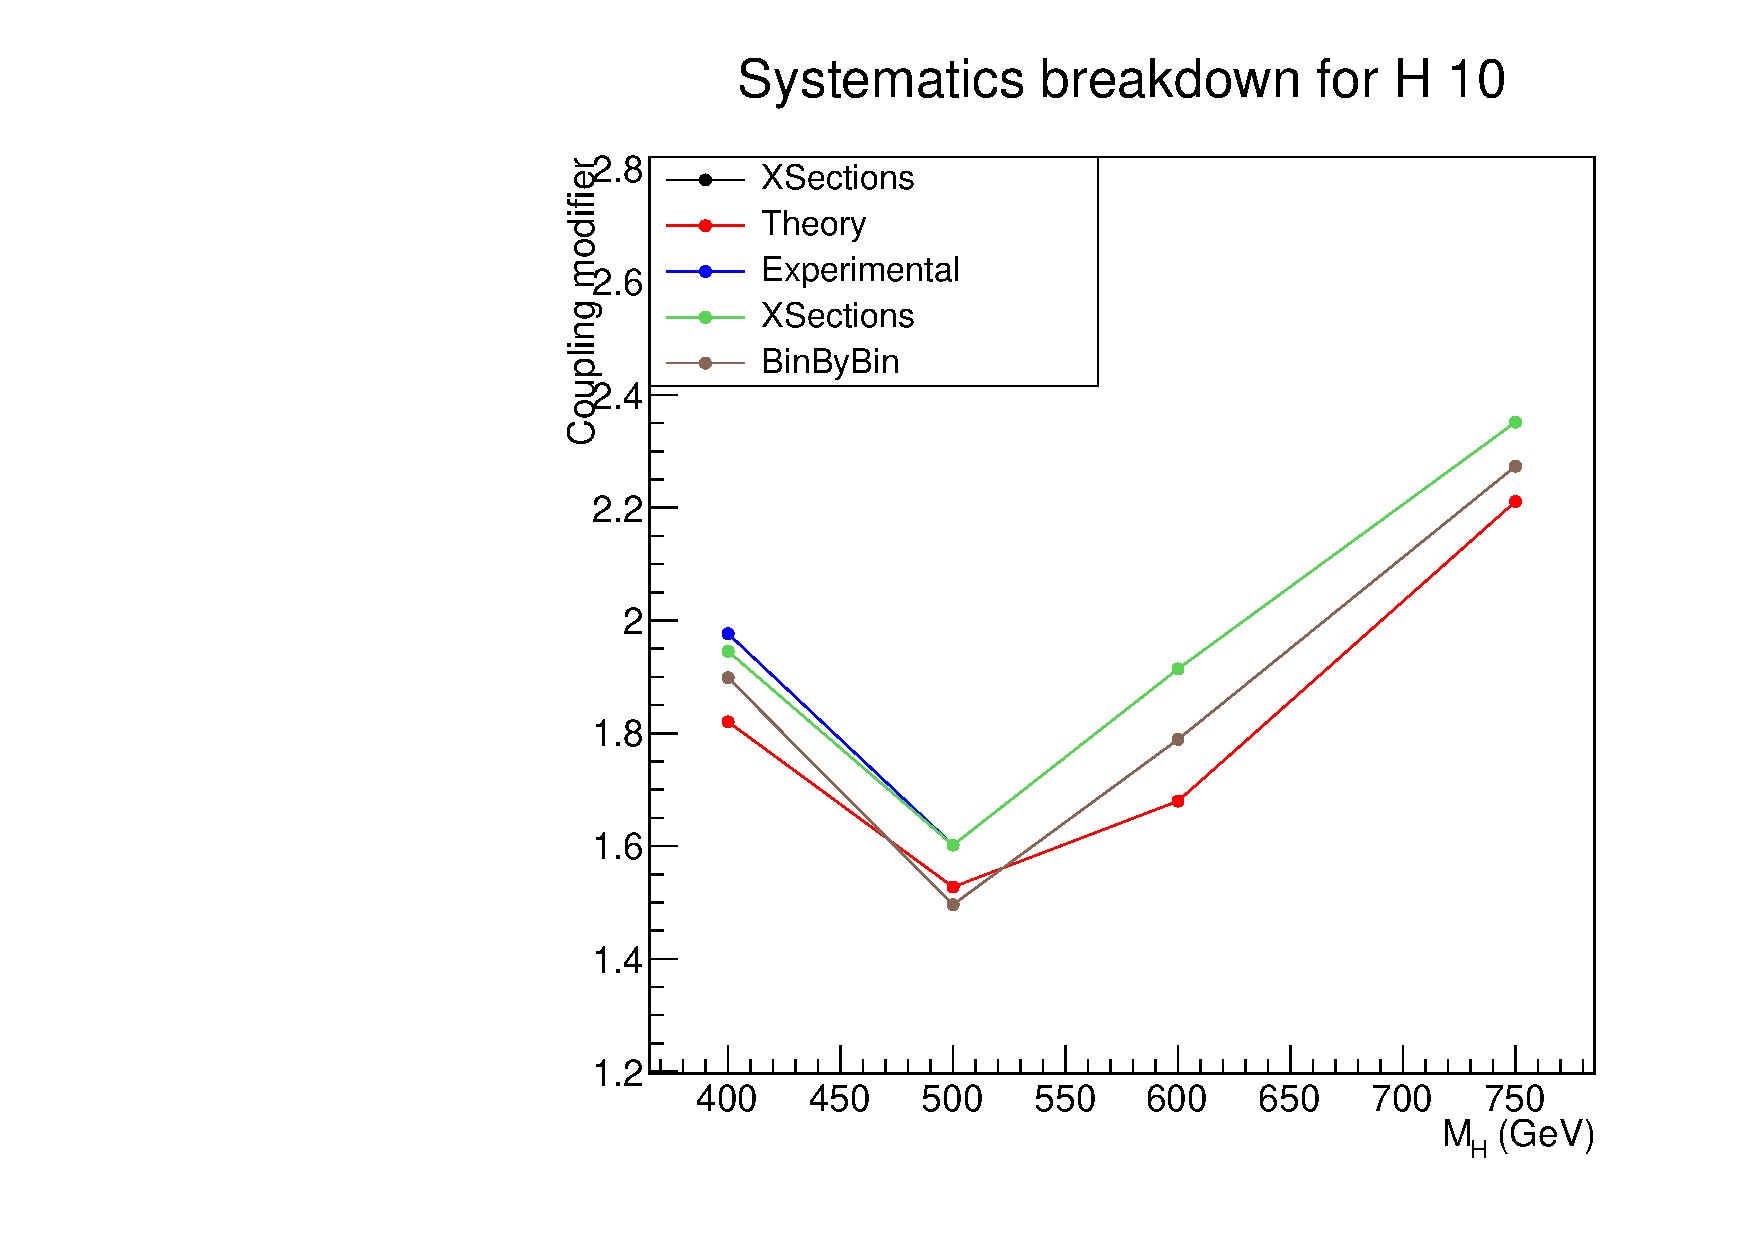
\includegraphics[width=0.35\textwidth,keepaspectratio=true]{fig/app5/breakdowns/generic_breakdown_H_10.pdf}
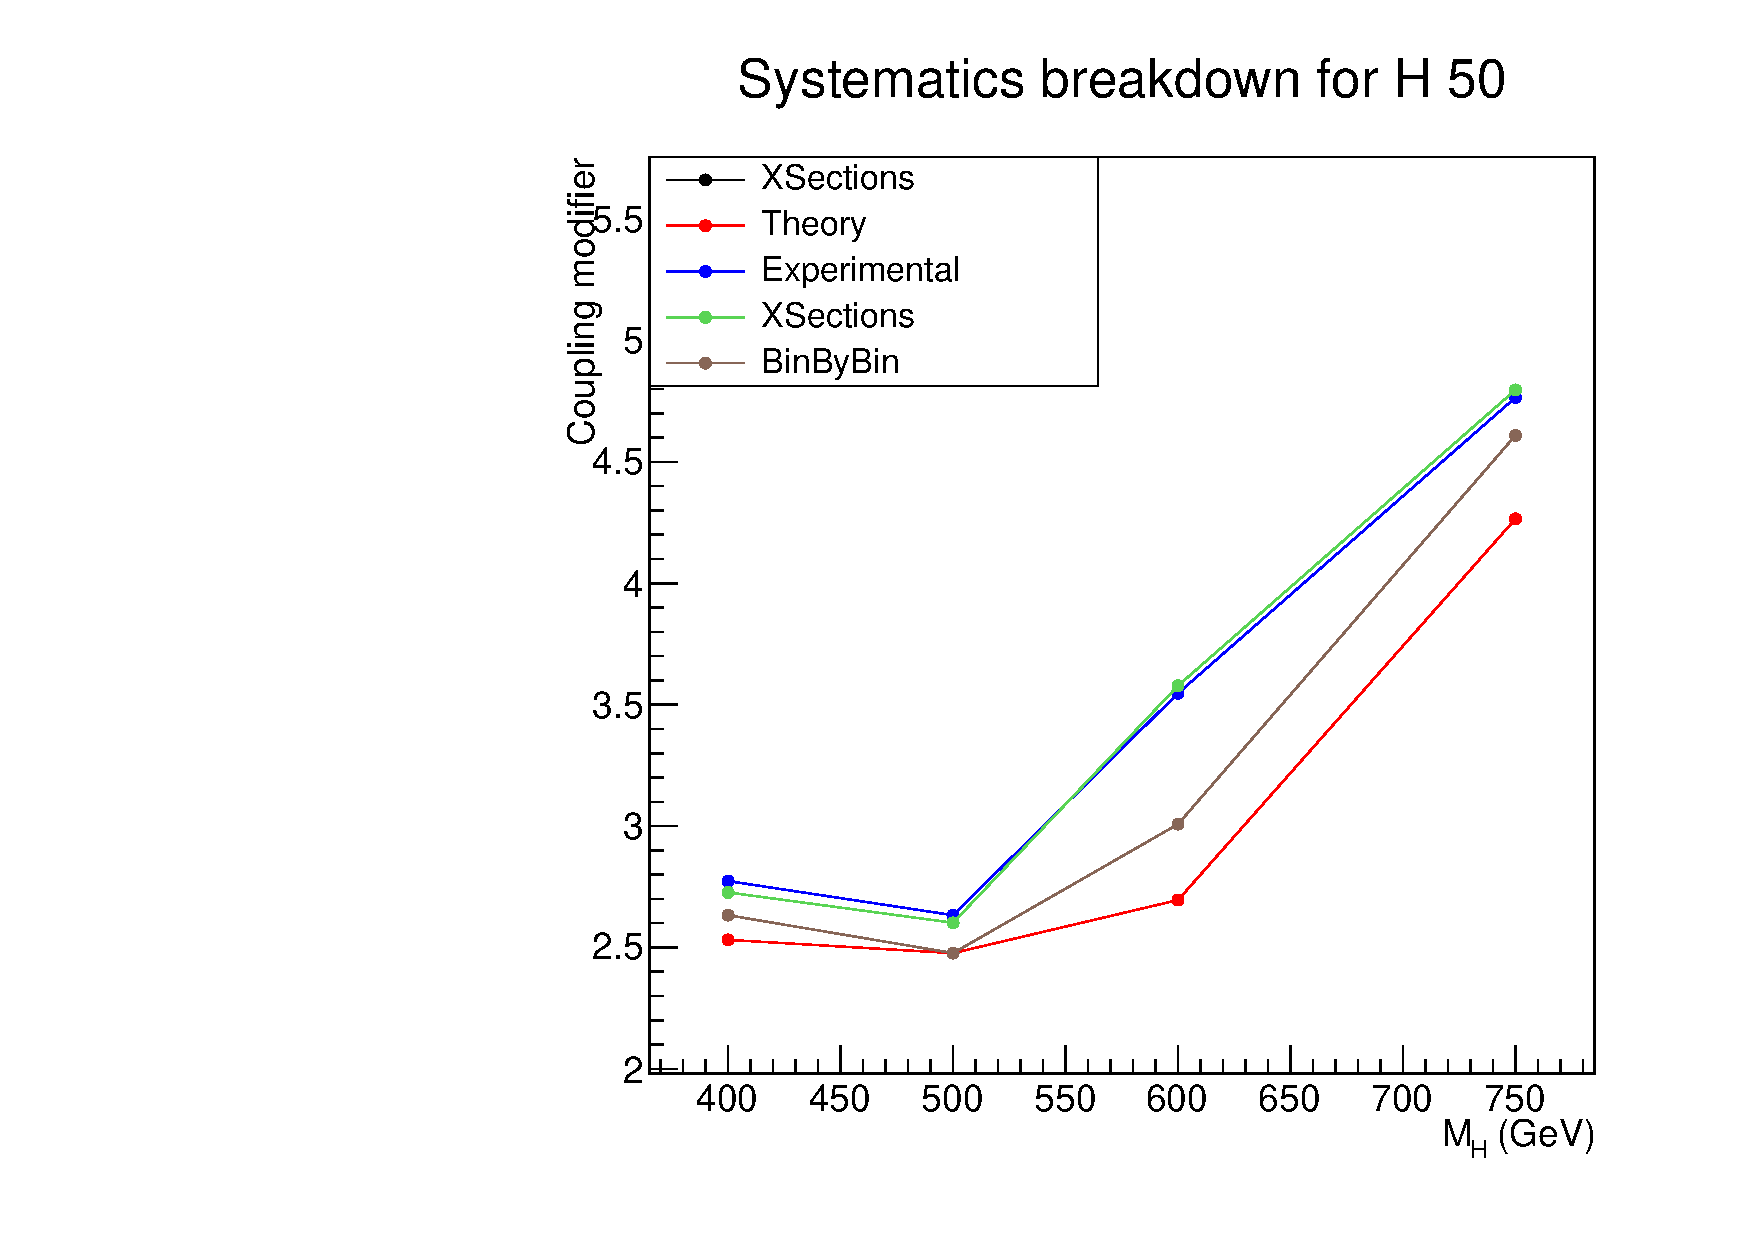
\includegraphics[width=0.35\textwidth,keepaspectratio=true]{fig/app5/breakdowns/generic_breakdown_H_50.pdf}
\caption{Expected upper limits on the coupling modifier with different groups of systematic uncertainties removed. The nominal limits are shown as the blue curve. The expected upper limits are shown for scalar signal as a function of mass for different values of the relative width, ranging from 2.5 to 50\%.}
\label{fig:breakdown_hwidths}
\end{figure}

\begin{figure}[!Hhtb]
\centering
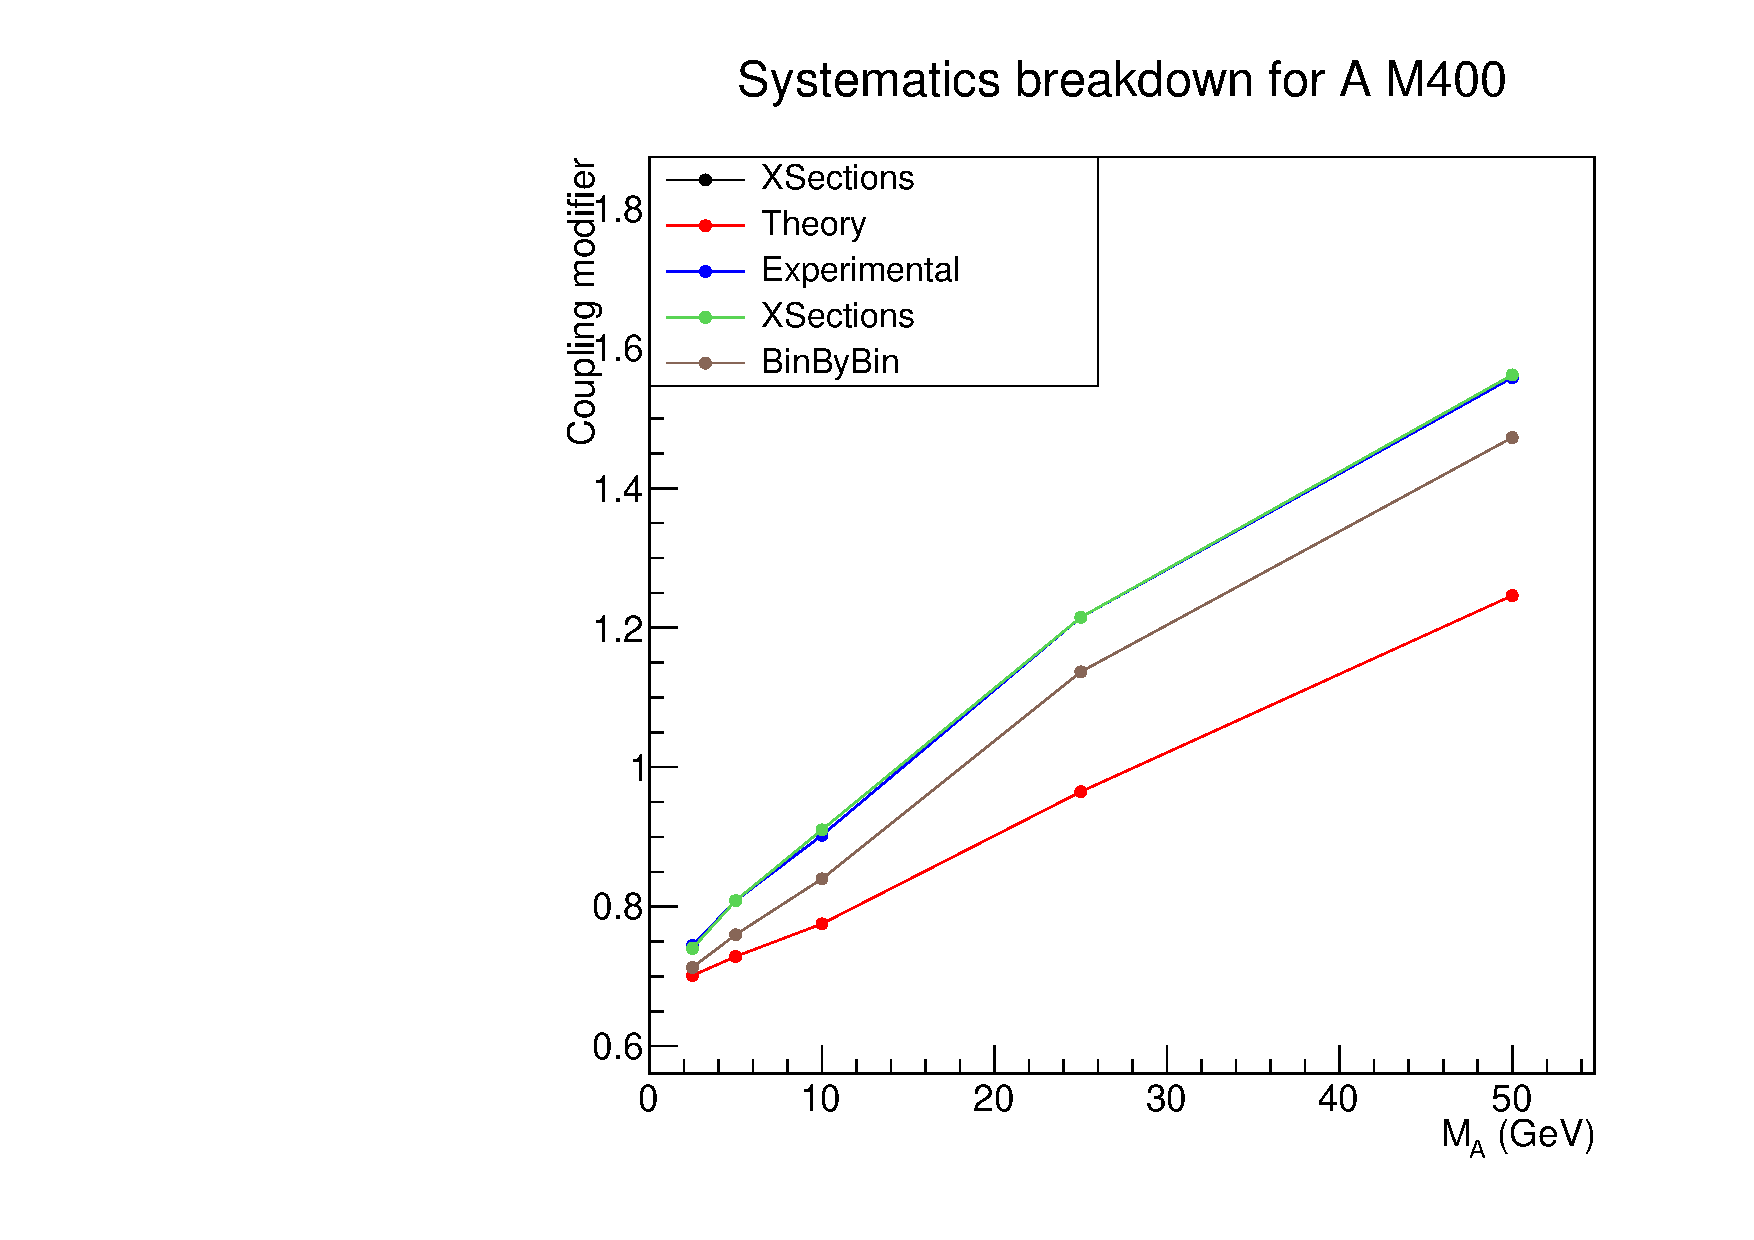
\includegraphics[width=0.35\textwidth,keepaspectratio=true]{fig/app5/breakdowns/generic_breakdown_A_M400.pdf}
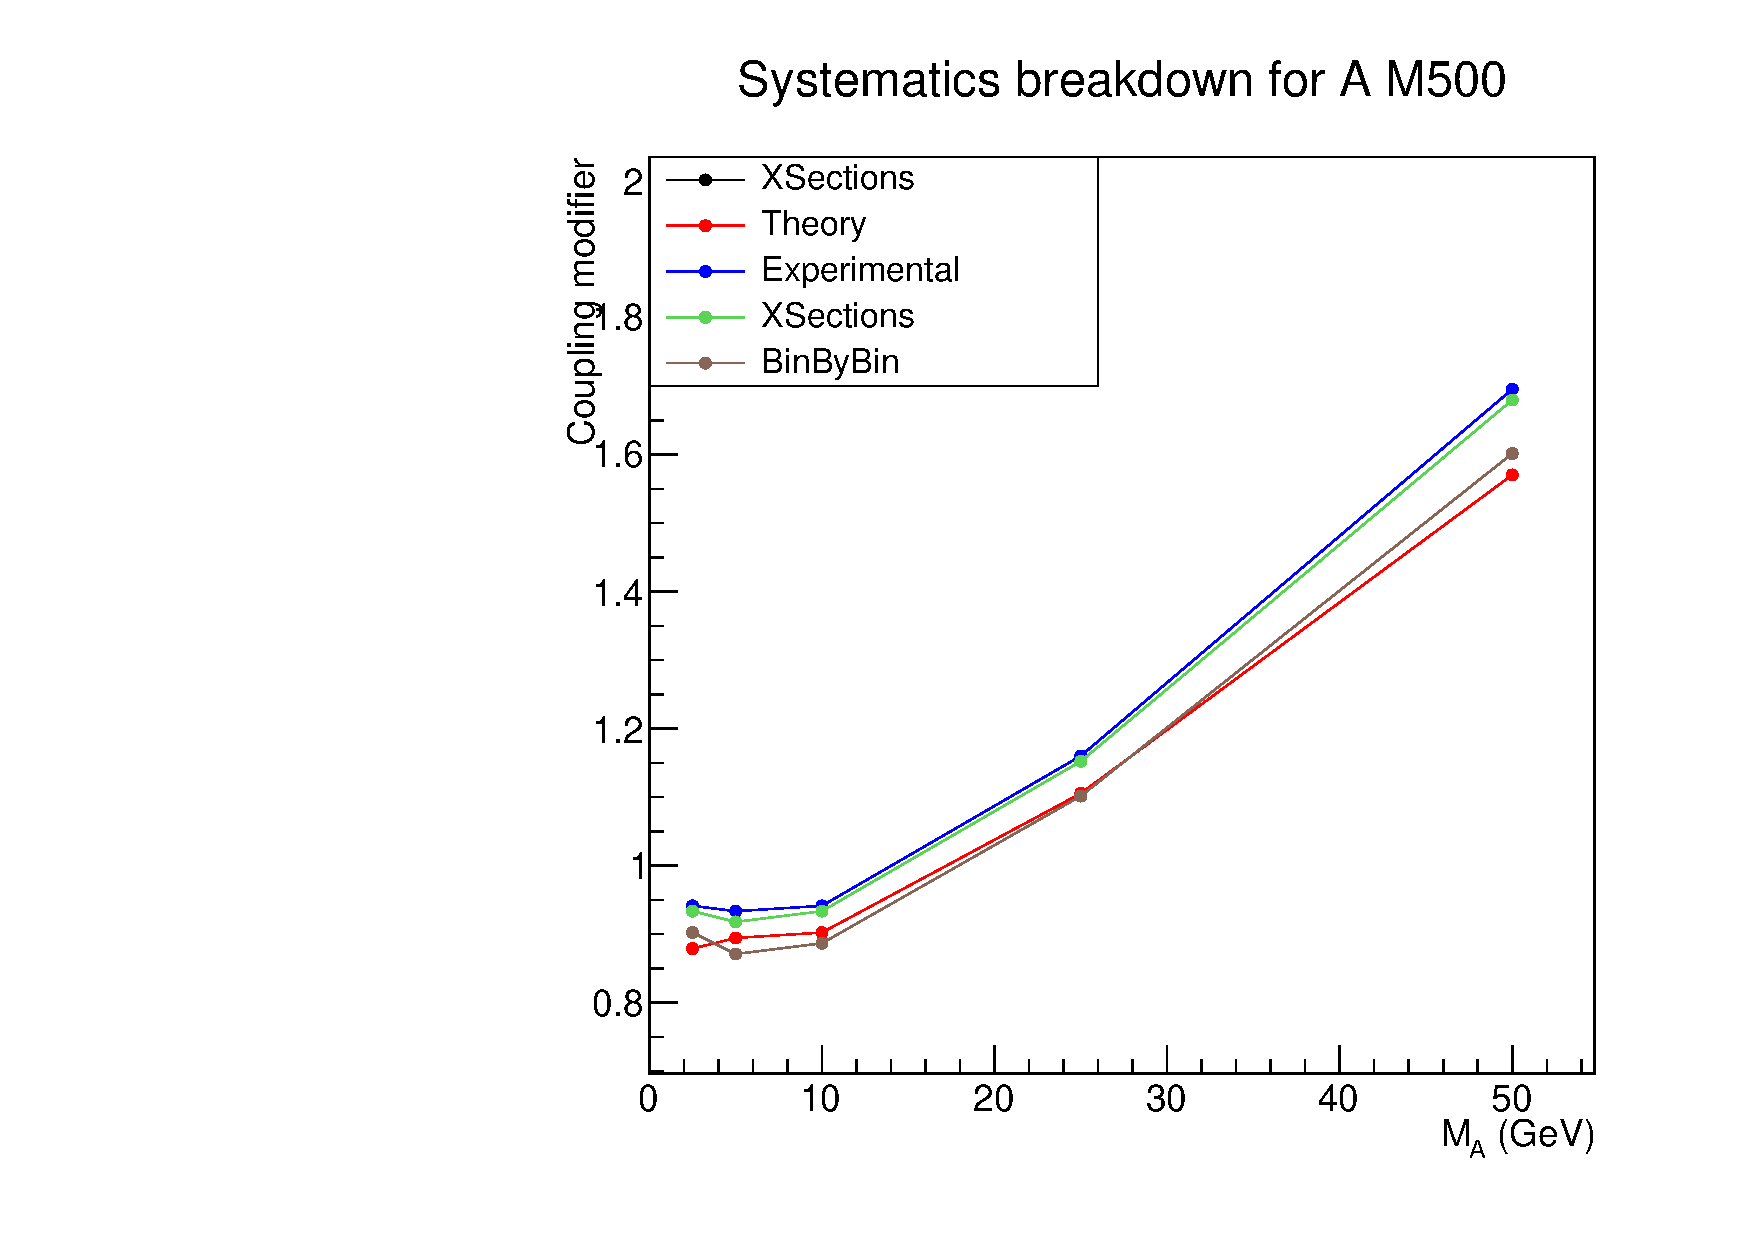
\includegraphics[width=0.35\textwidth,keepaspectratio=true]{fig/app5/breakdowns/generic_breakdown_A_M500.pdf}
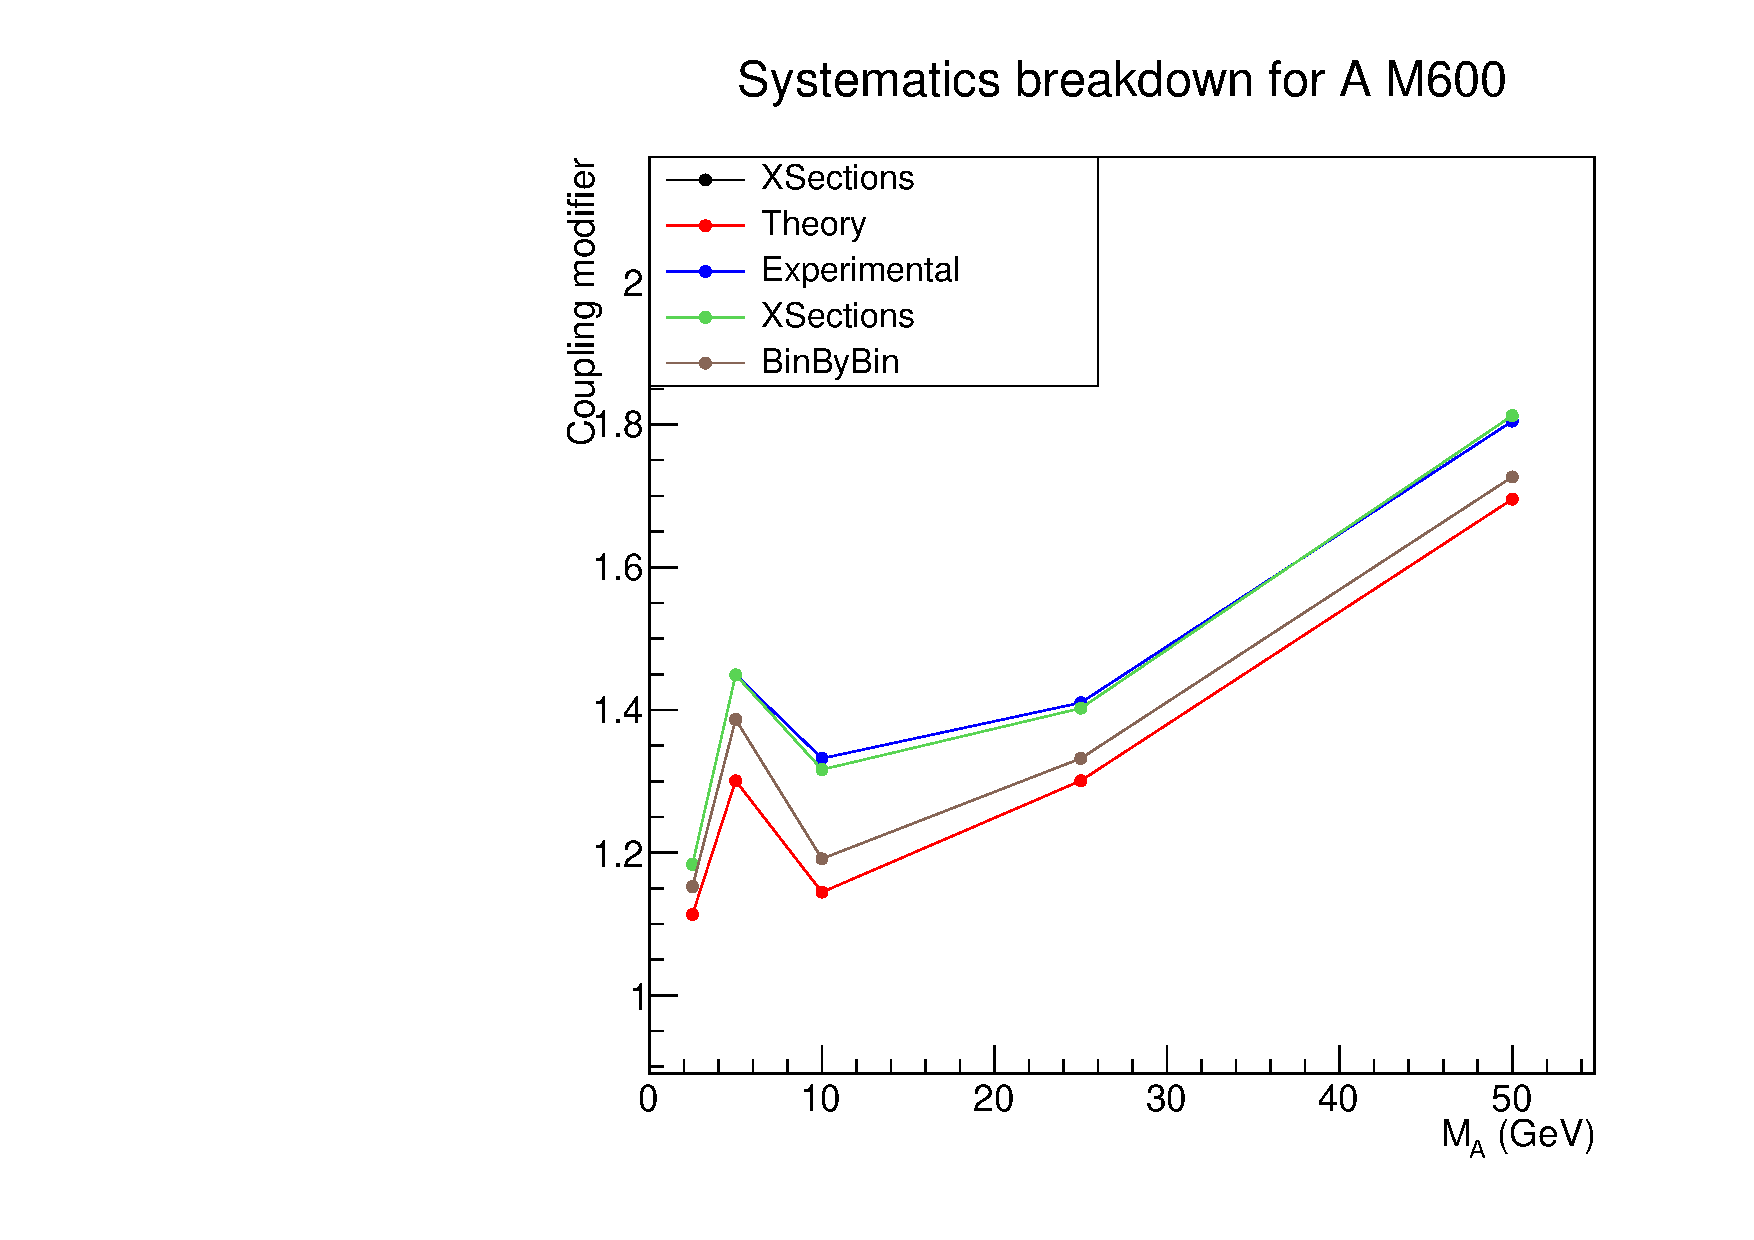
\includegraphics[width=0.35\textwidth,keepaspectratio=true]{fig/app5/breakdowns/generic_breakdown_A_M600.pdf}
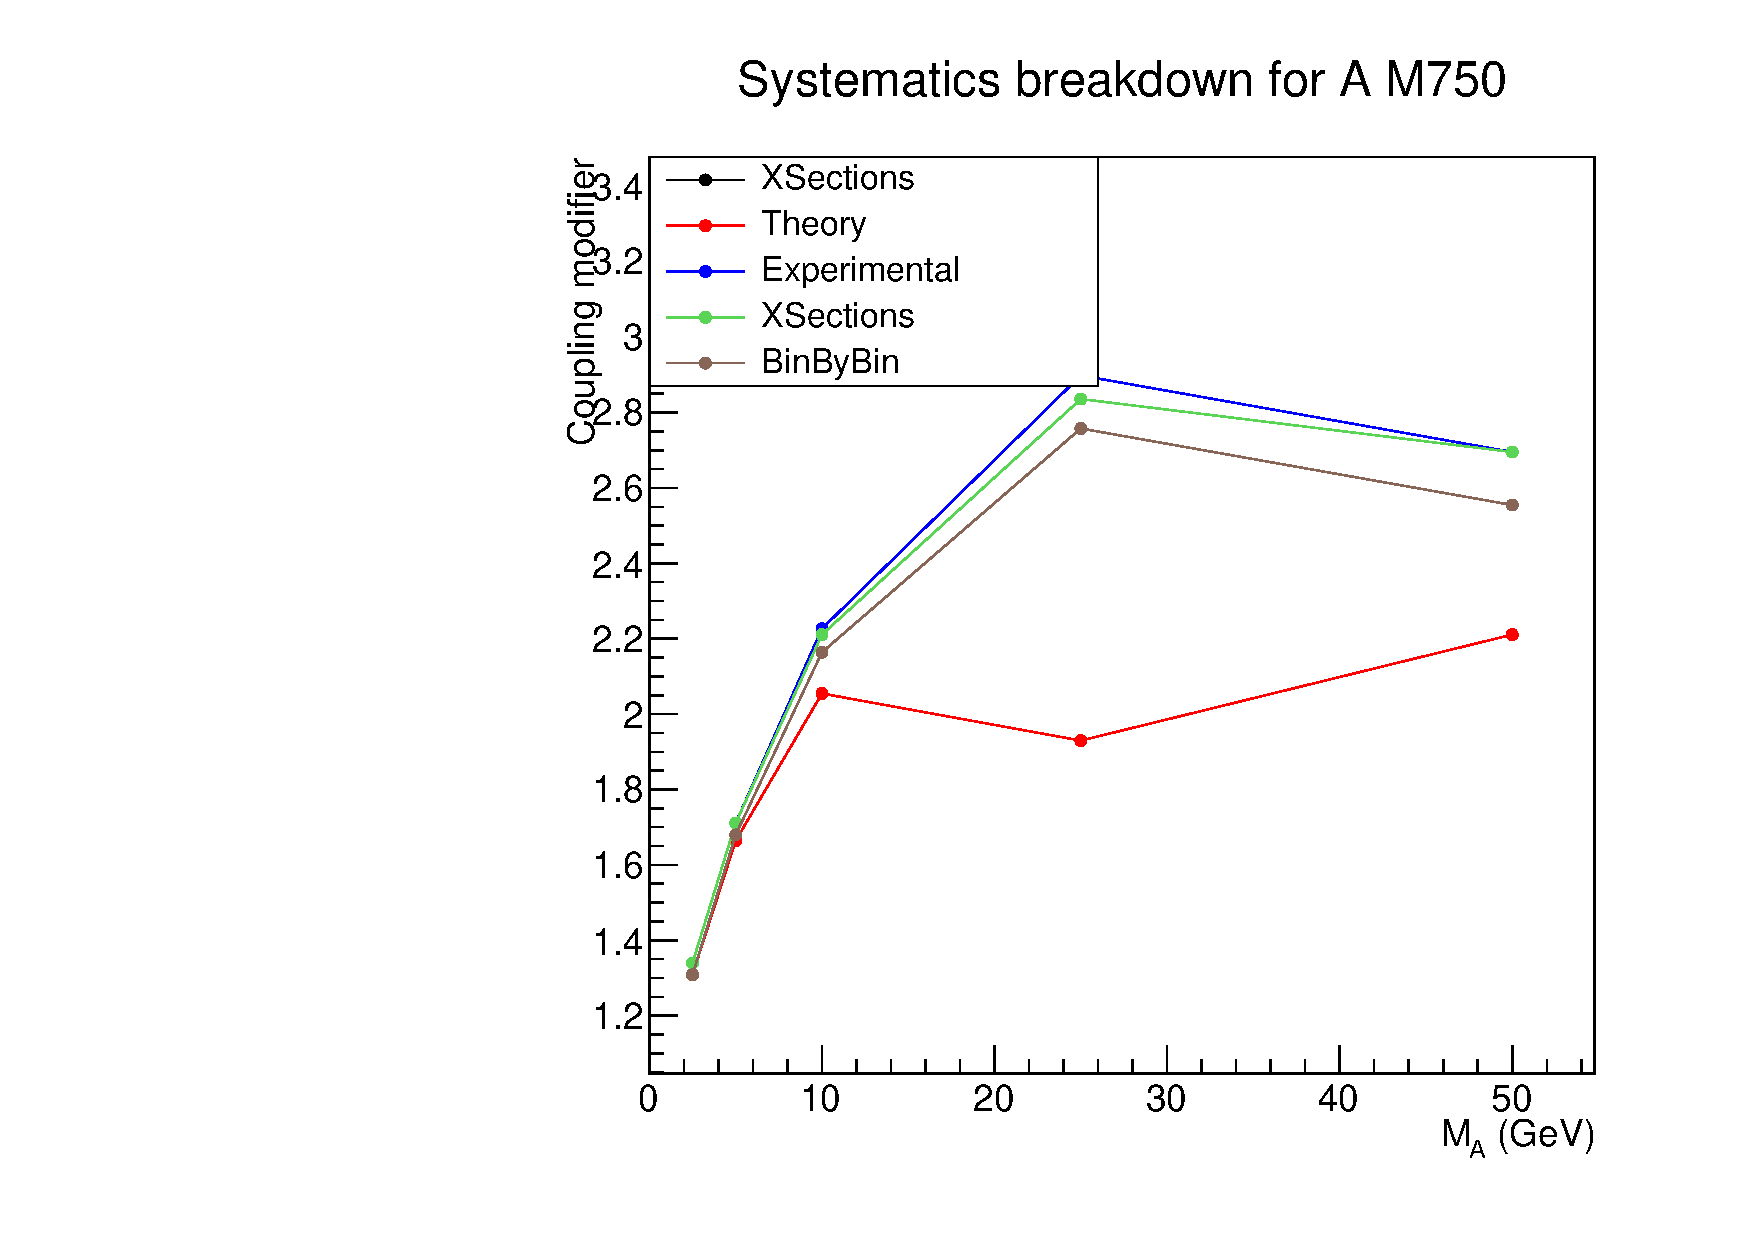
\includegraphics[width=0.35\textwidth,keepaspectratio=true]{fig/app5/breakdowns/generic_breakdown_A_M750.pdf}
\caption{Expected upper limits on the coupling modifier with different groups of systematic uncertainties removed. The nominal limits are shown as the blue curve. The expected upper limits are shown for pseudoscalar signal as a function of relative width for different values of the mass, ranging from 400 to 750~GeV.}
\label{fig:breakdown_amass}
\end{figure}


\begin{figure}[!Hhtb]
\centering
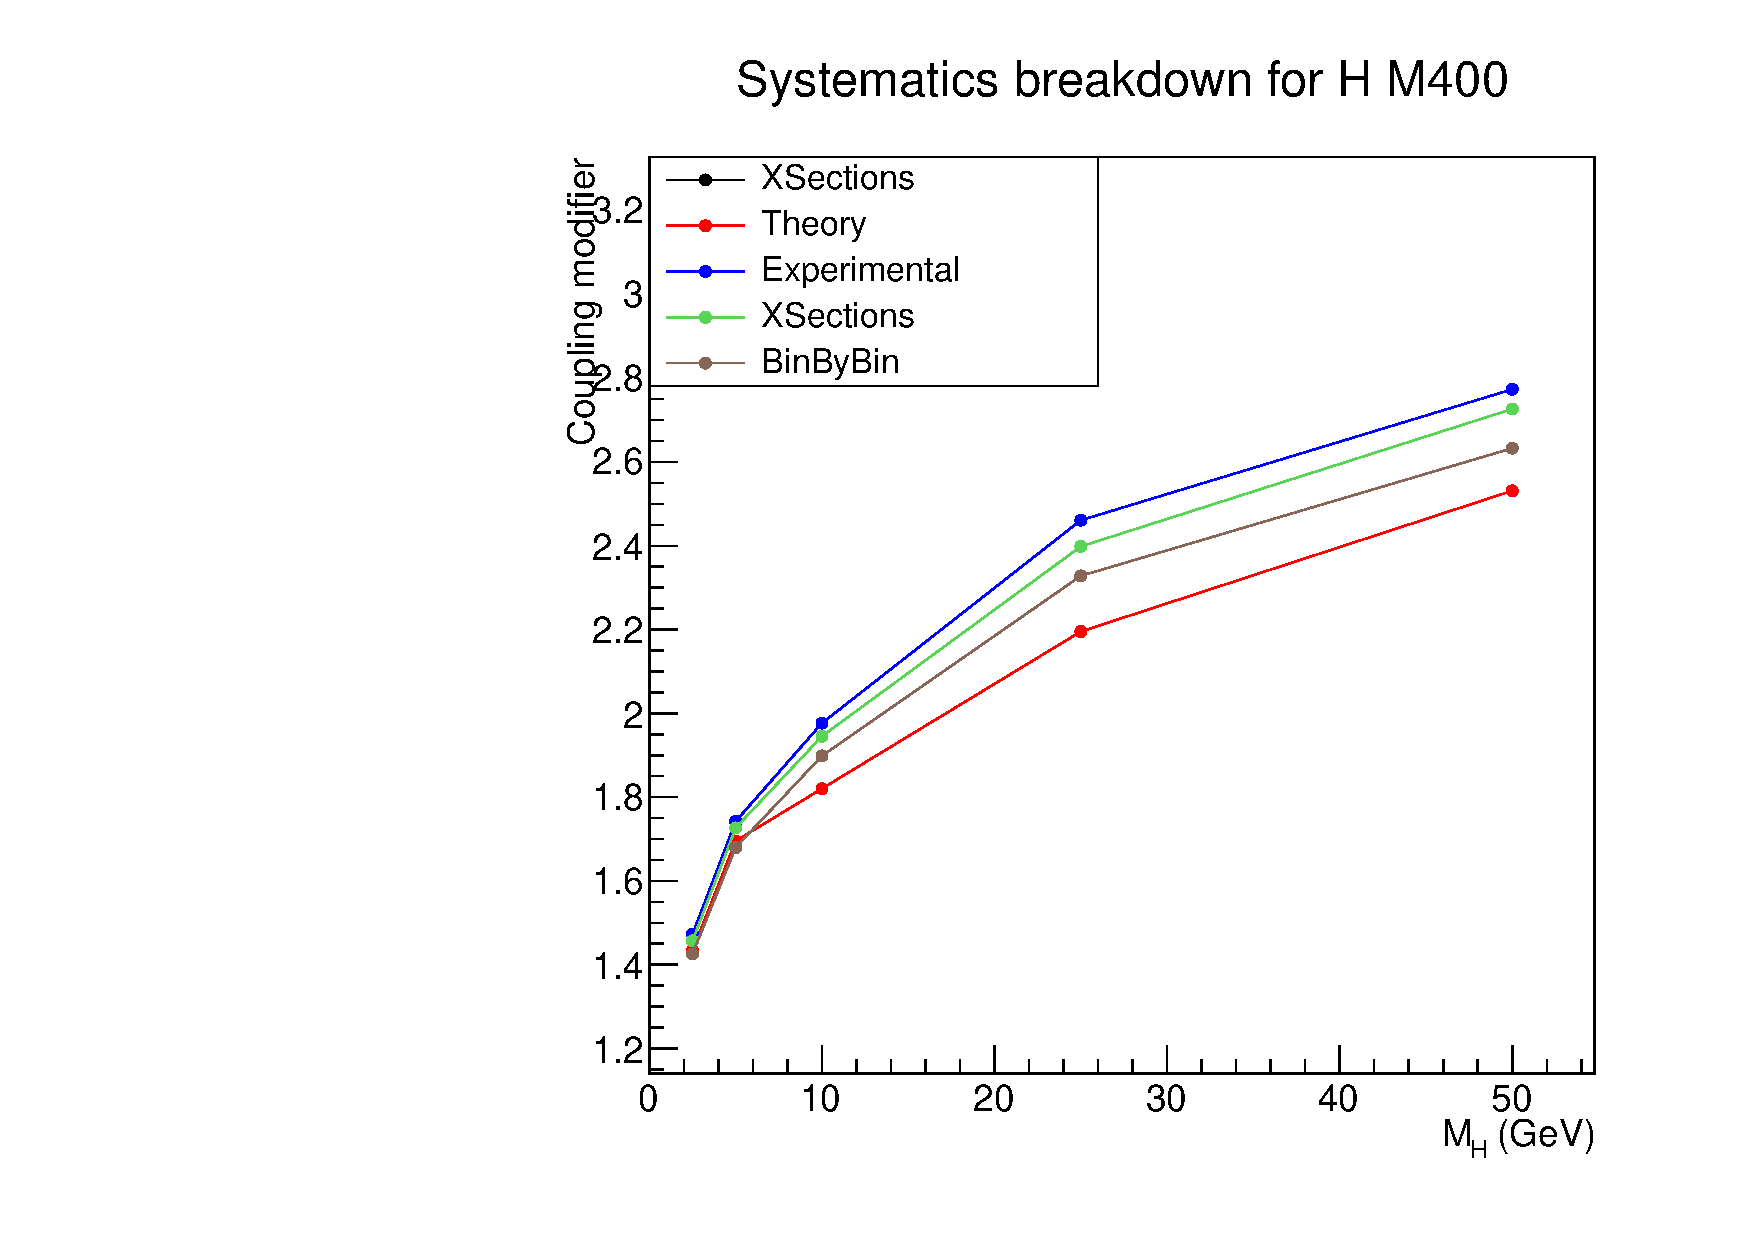
\includegraphics[width=0.35\textwidth,keepaspectratio=true]{fig/app5/breakdowns/generic_breakdown_H_M400.pdf}
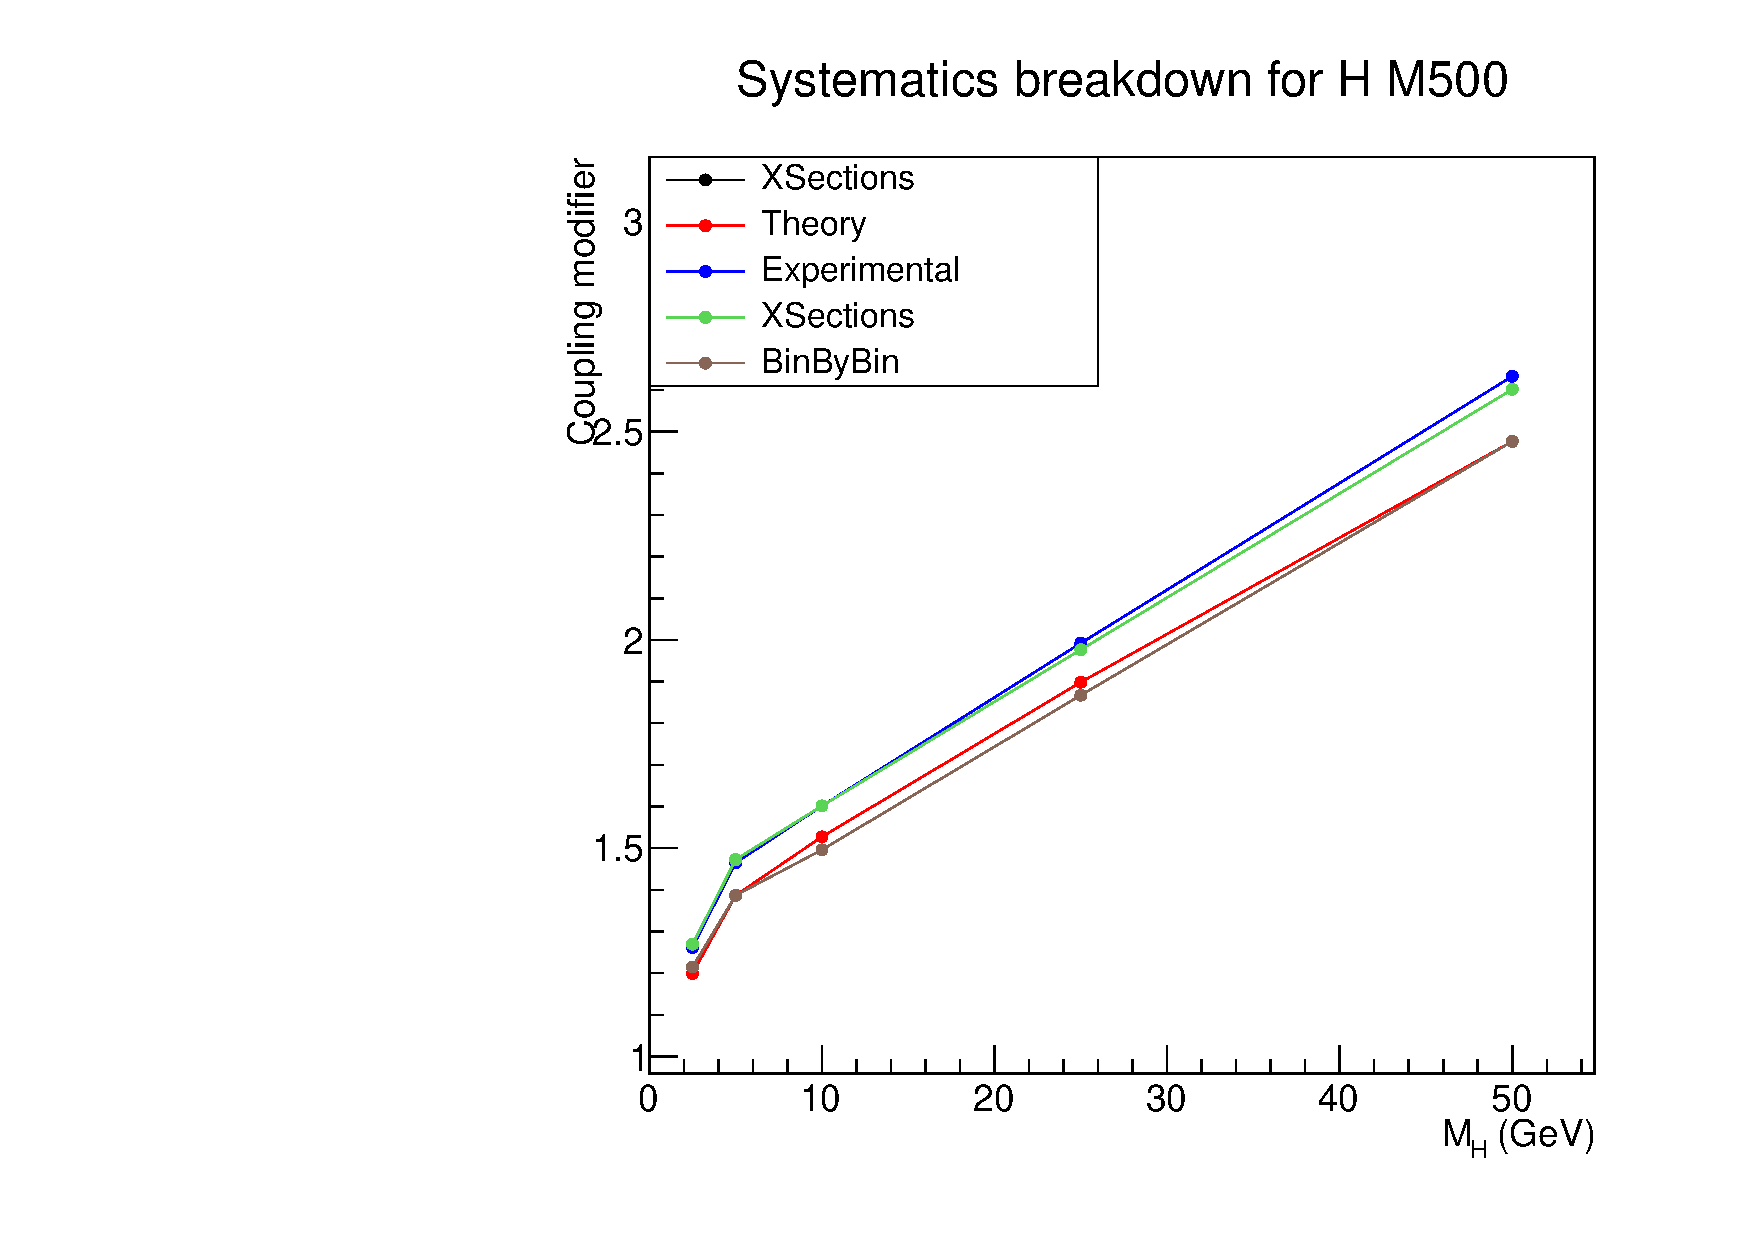
\includegraphics[width=0.35\textwidth,keepaspectratio=true]{fig/app5/breakdowns/generic_breakdown_H_M500.pdf}
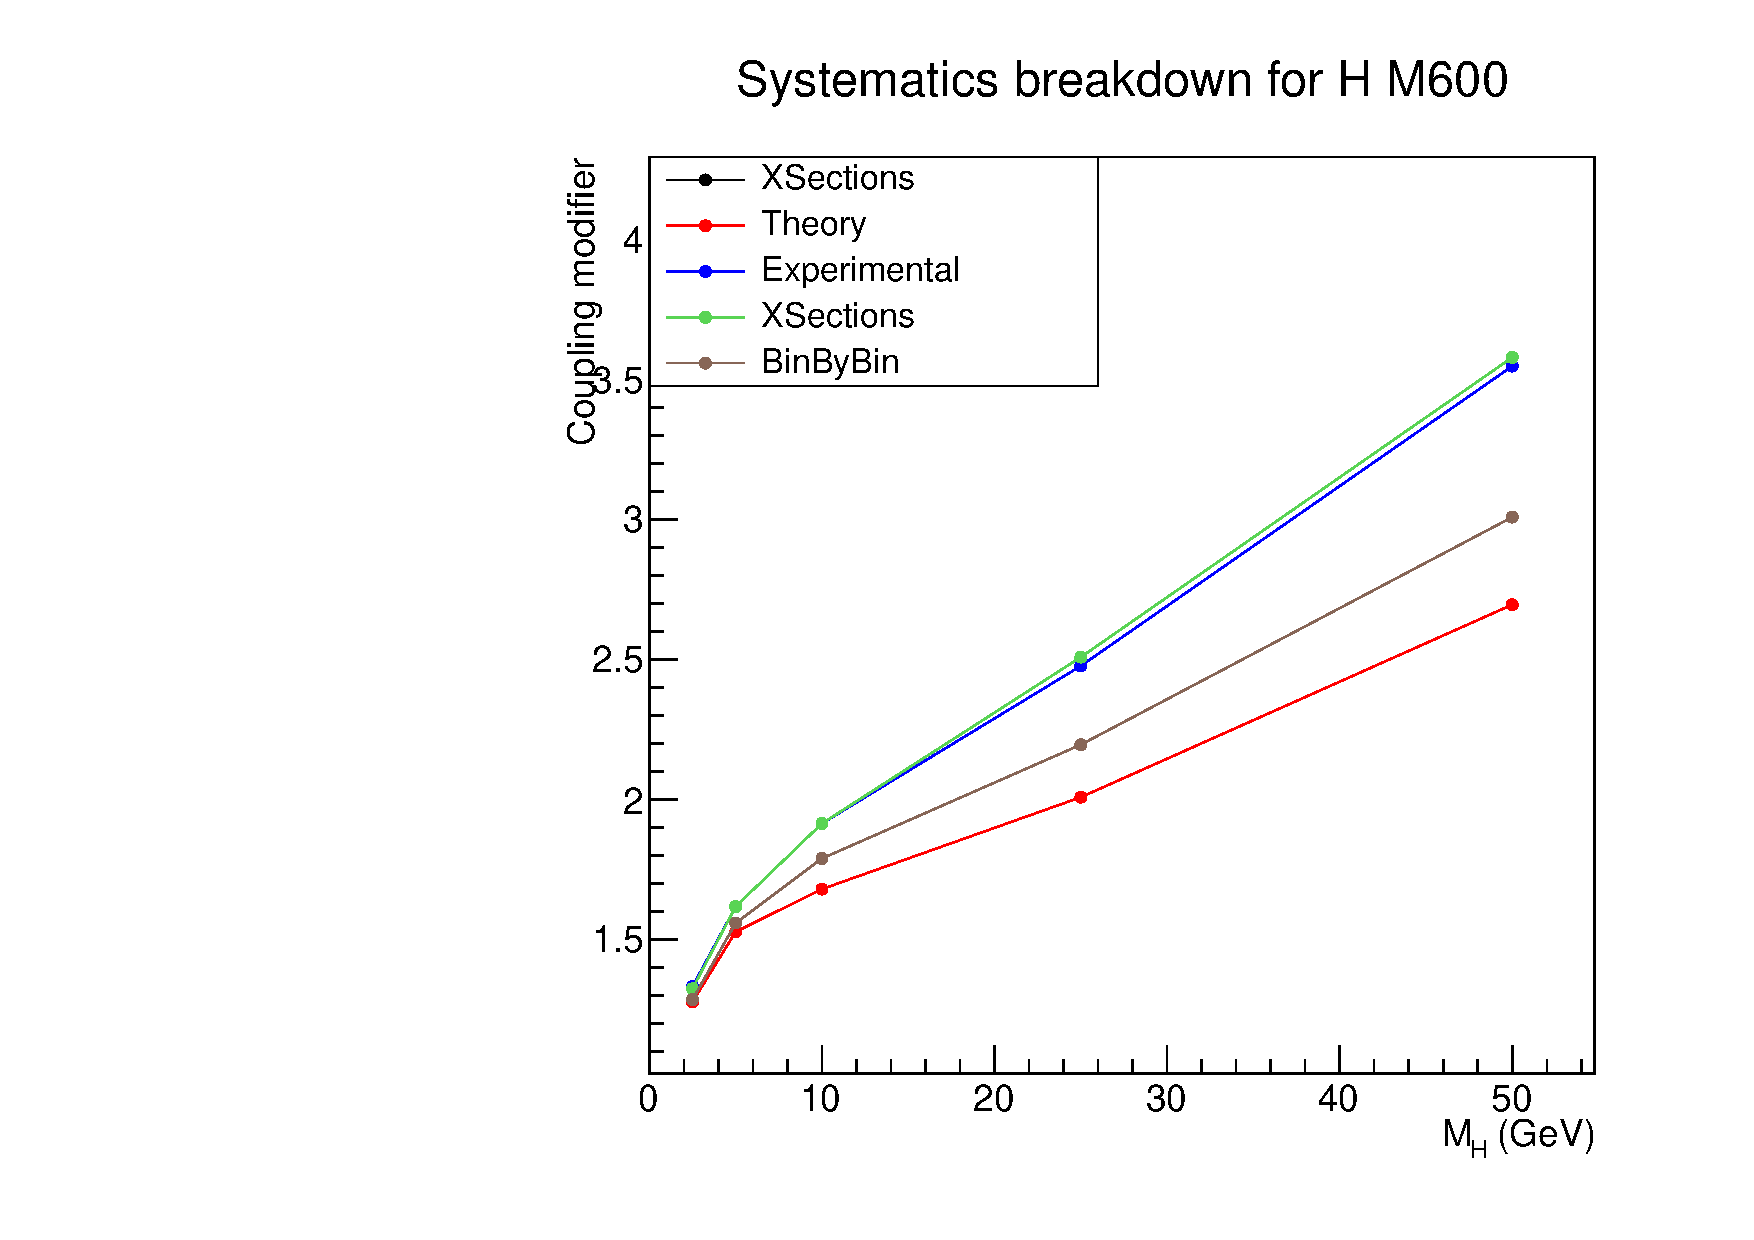
\includegraphics[width=0.35\textwidth,keepaspectratio=true]{fig/app5/breakdowns/generic_breakdown_H_M600.pdf}
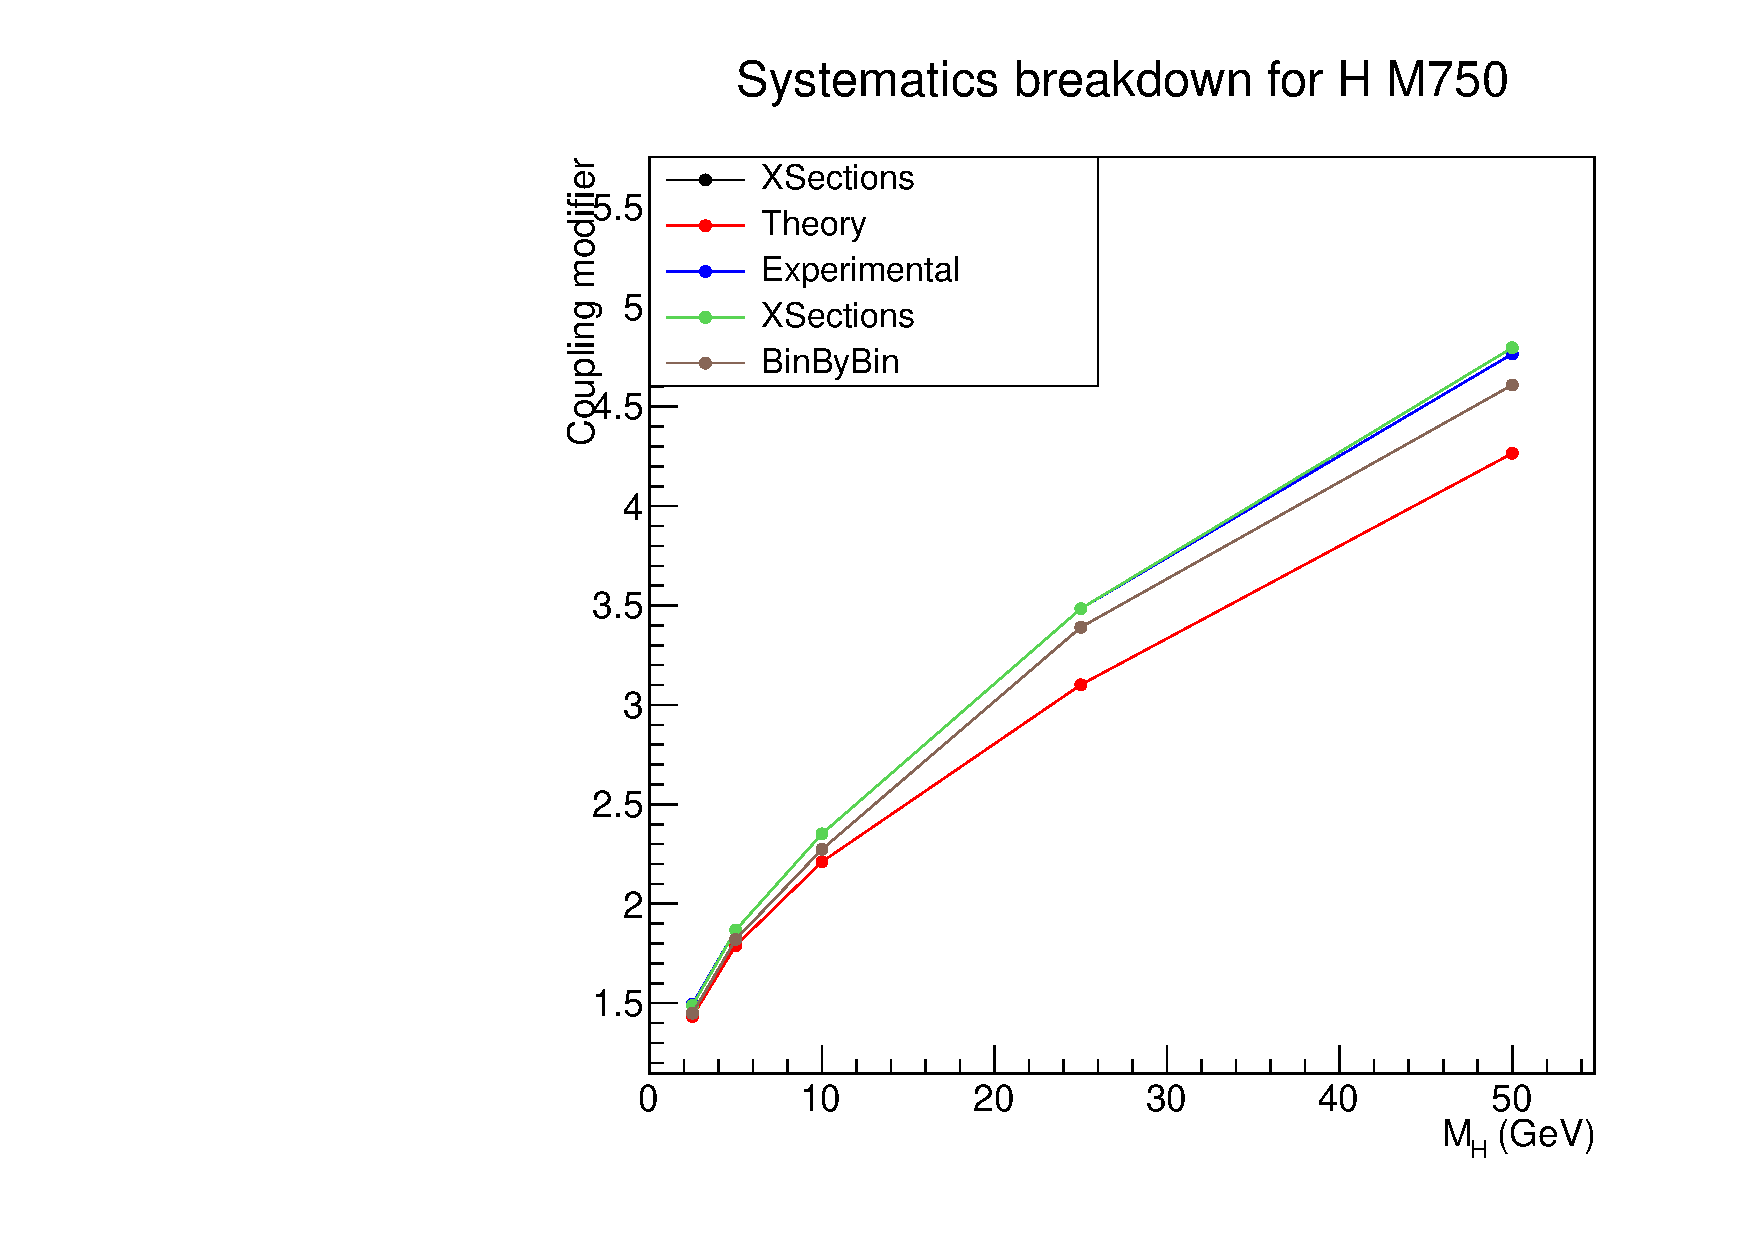
\includegraphics[width=0.35\textwidth,keepaspectratio=true]{fig/app5/breakdowns/generic_breakdown_H_M750.pdf}
\caption{Expected upper limits on the coupling modifier with different groups of systematic uncertainties removed. The nominal limits are shown as the blue curve. The expected upper limits are shown for pseudoscalar signal as a function of relative width for different values of the mass, ranging from 400 to 750~GeV.}
\label{fig:breakdown_hmass}
\end{figure}

\begin{figure}[!Hhtb]
\centering
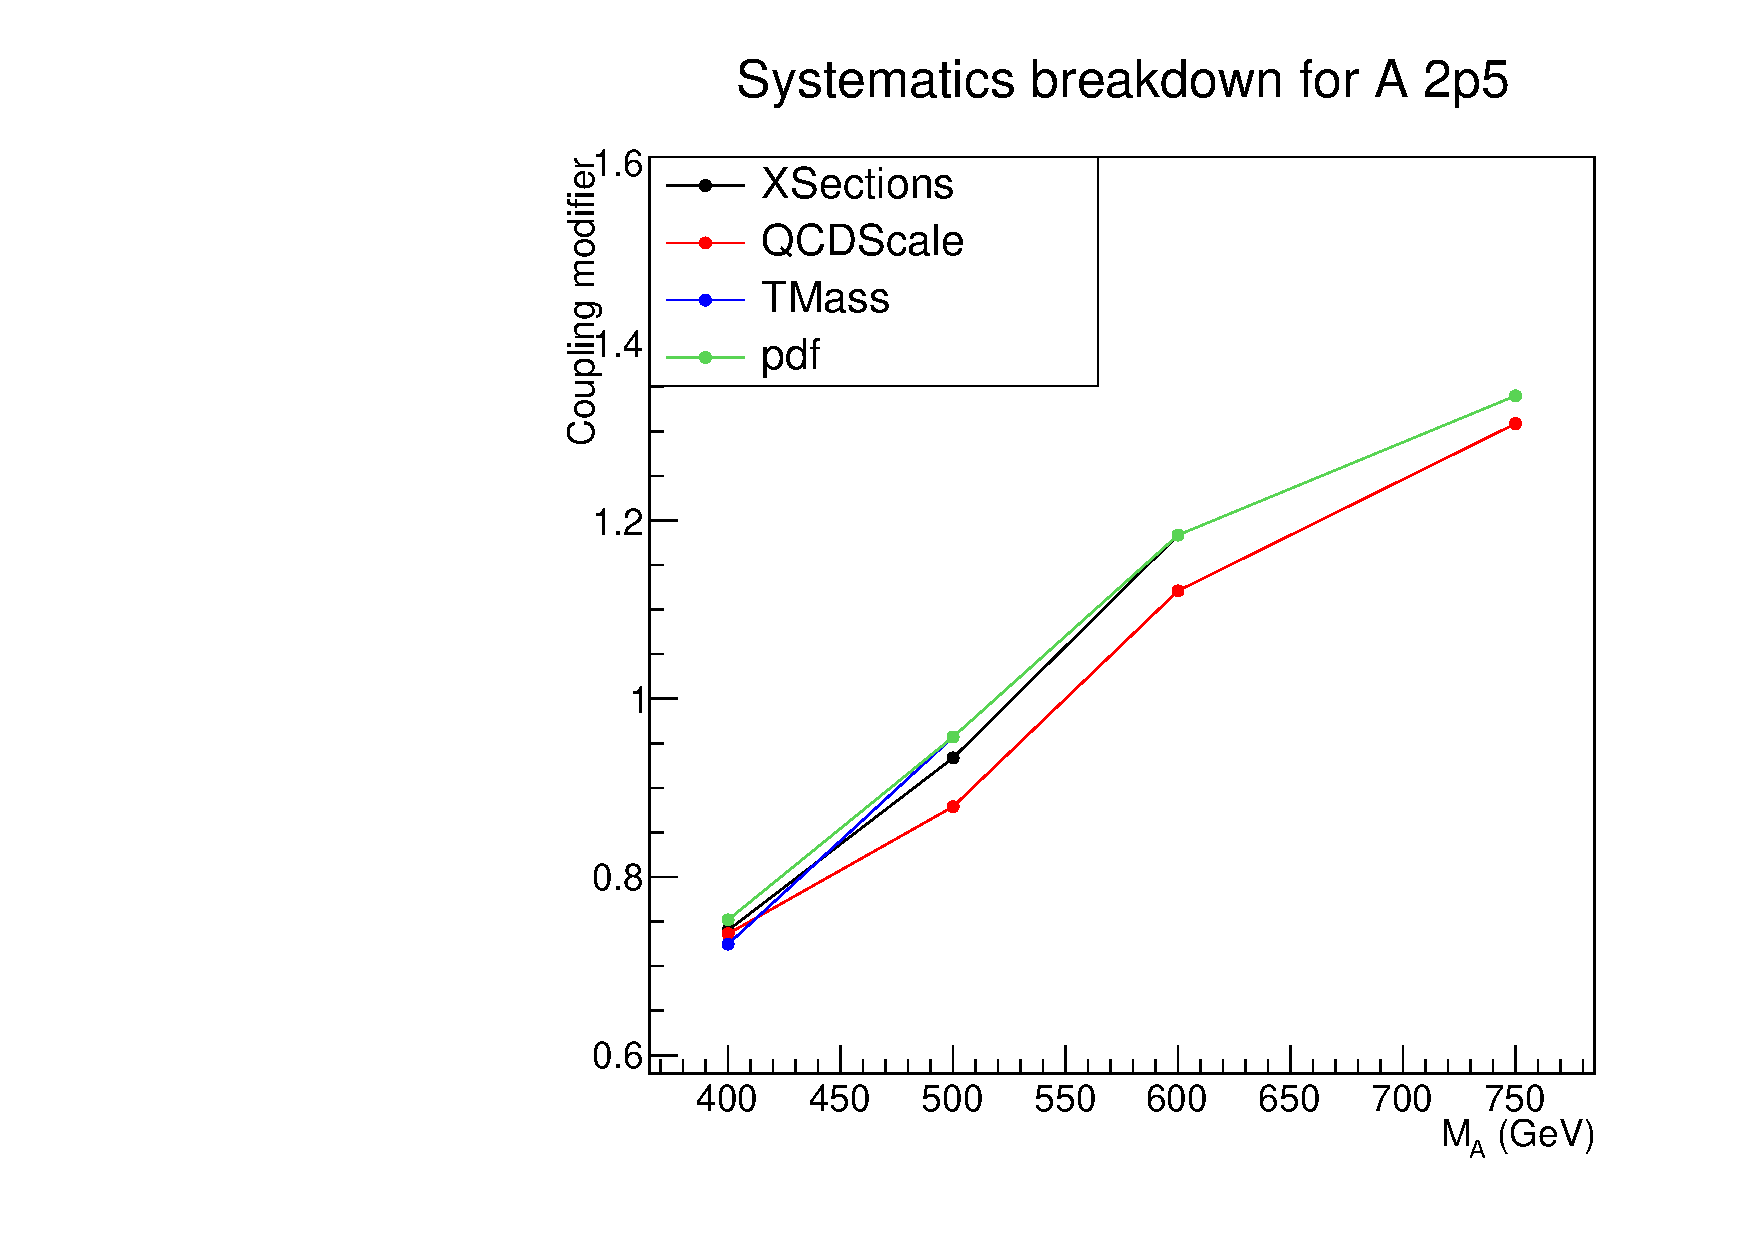
\includegraphics[width=0.35\textwidth,keepaspectratio=true]{fig/app5/breakdowns/theory_breakdown_A_2p5.pdf}
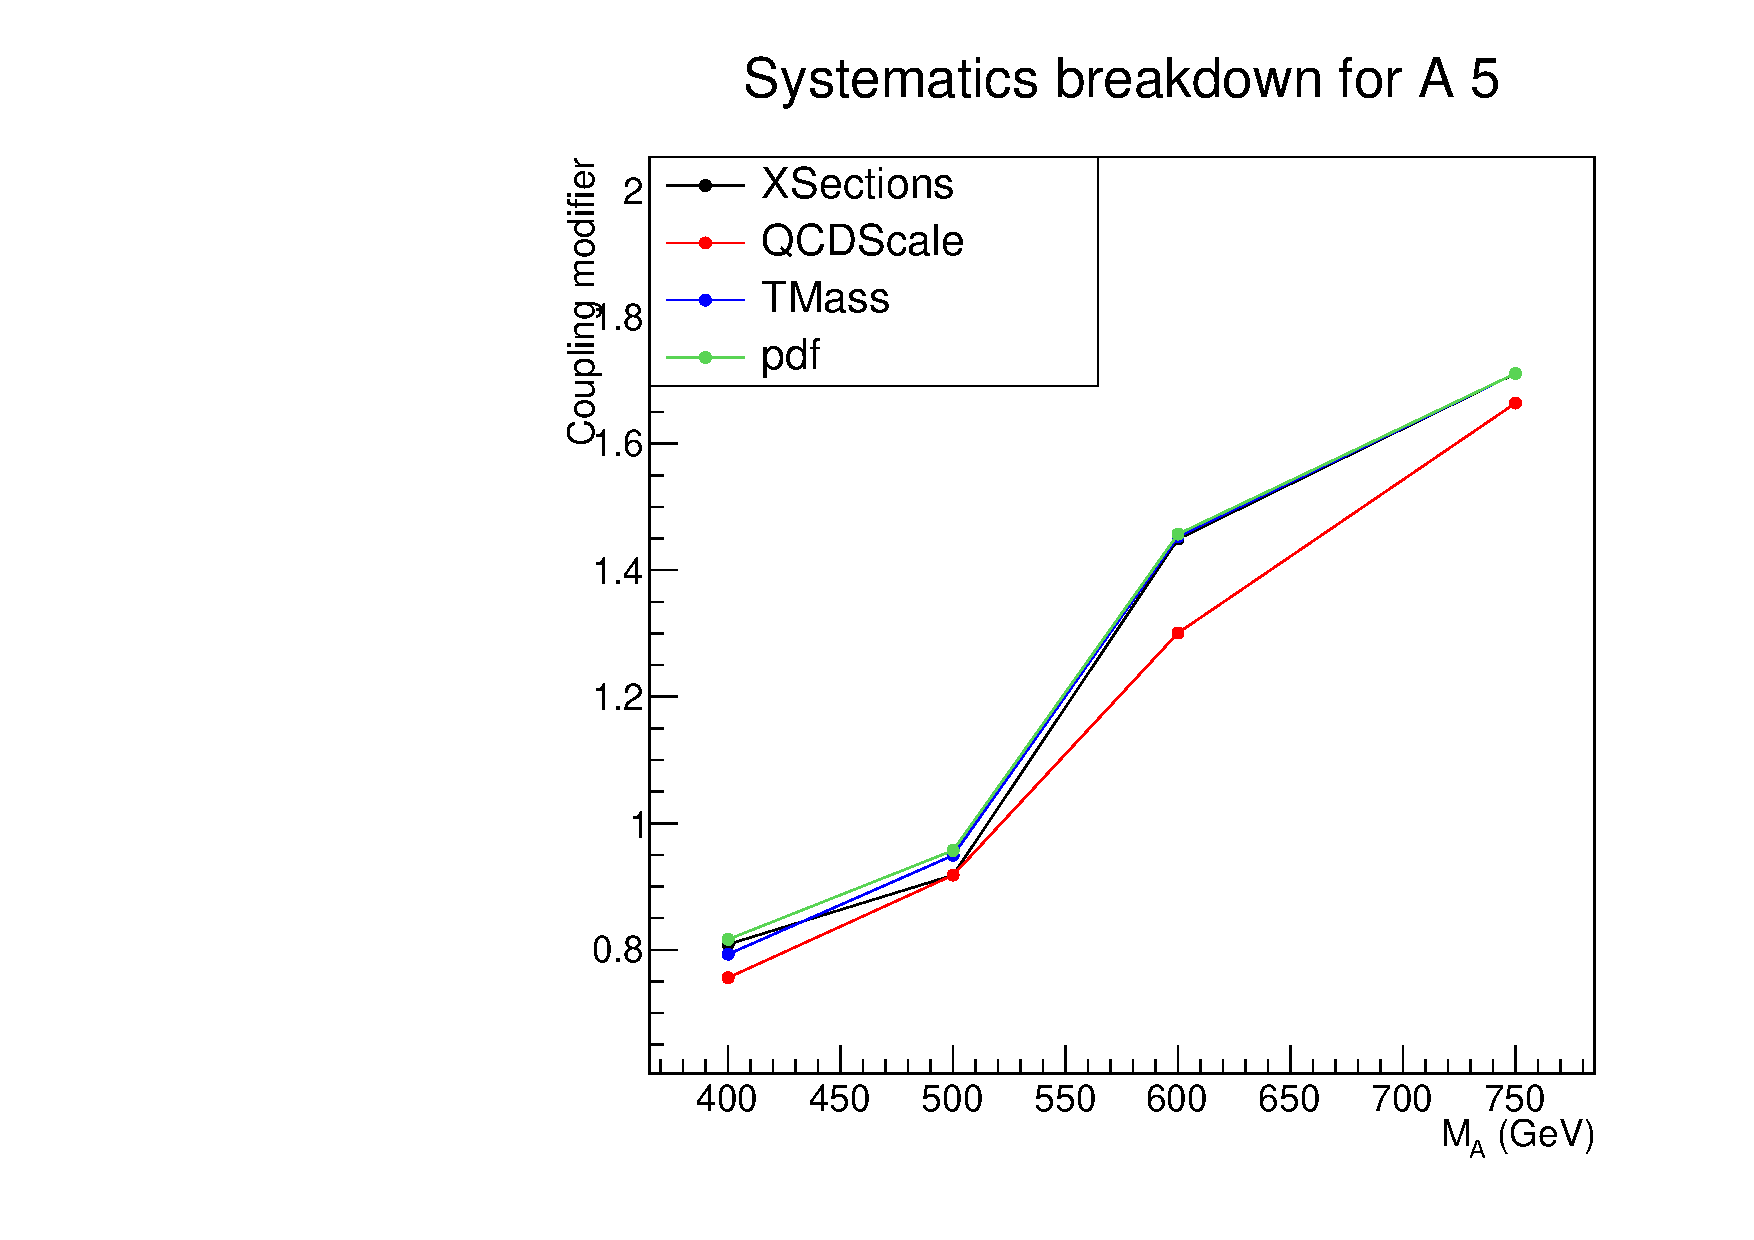
\includegraphics[width=0.35\textwidth,keepaspectratio=true]{fig/app5/breakdowns/theory_breakdown_A_5.pdf}
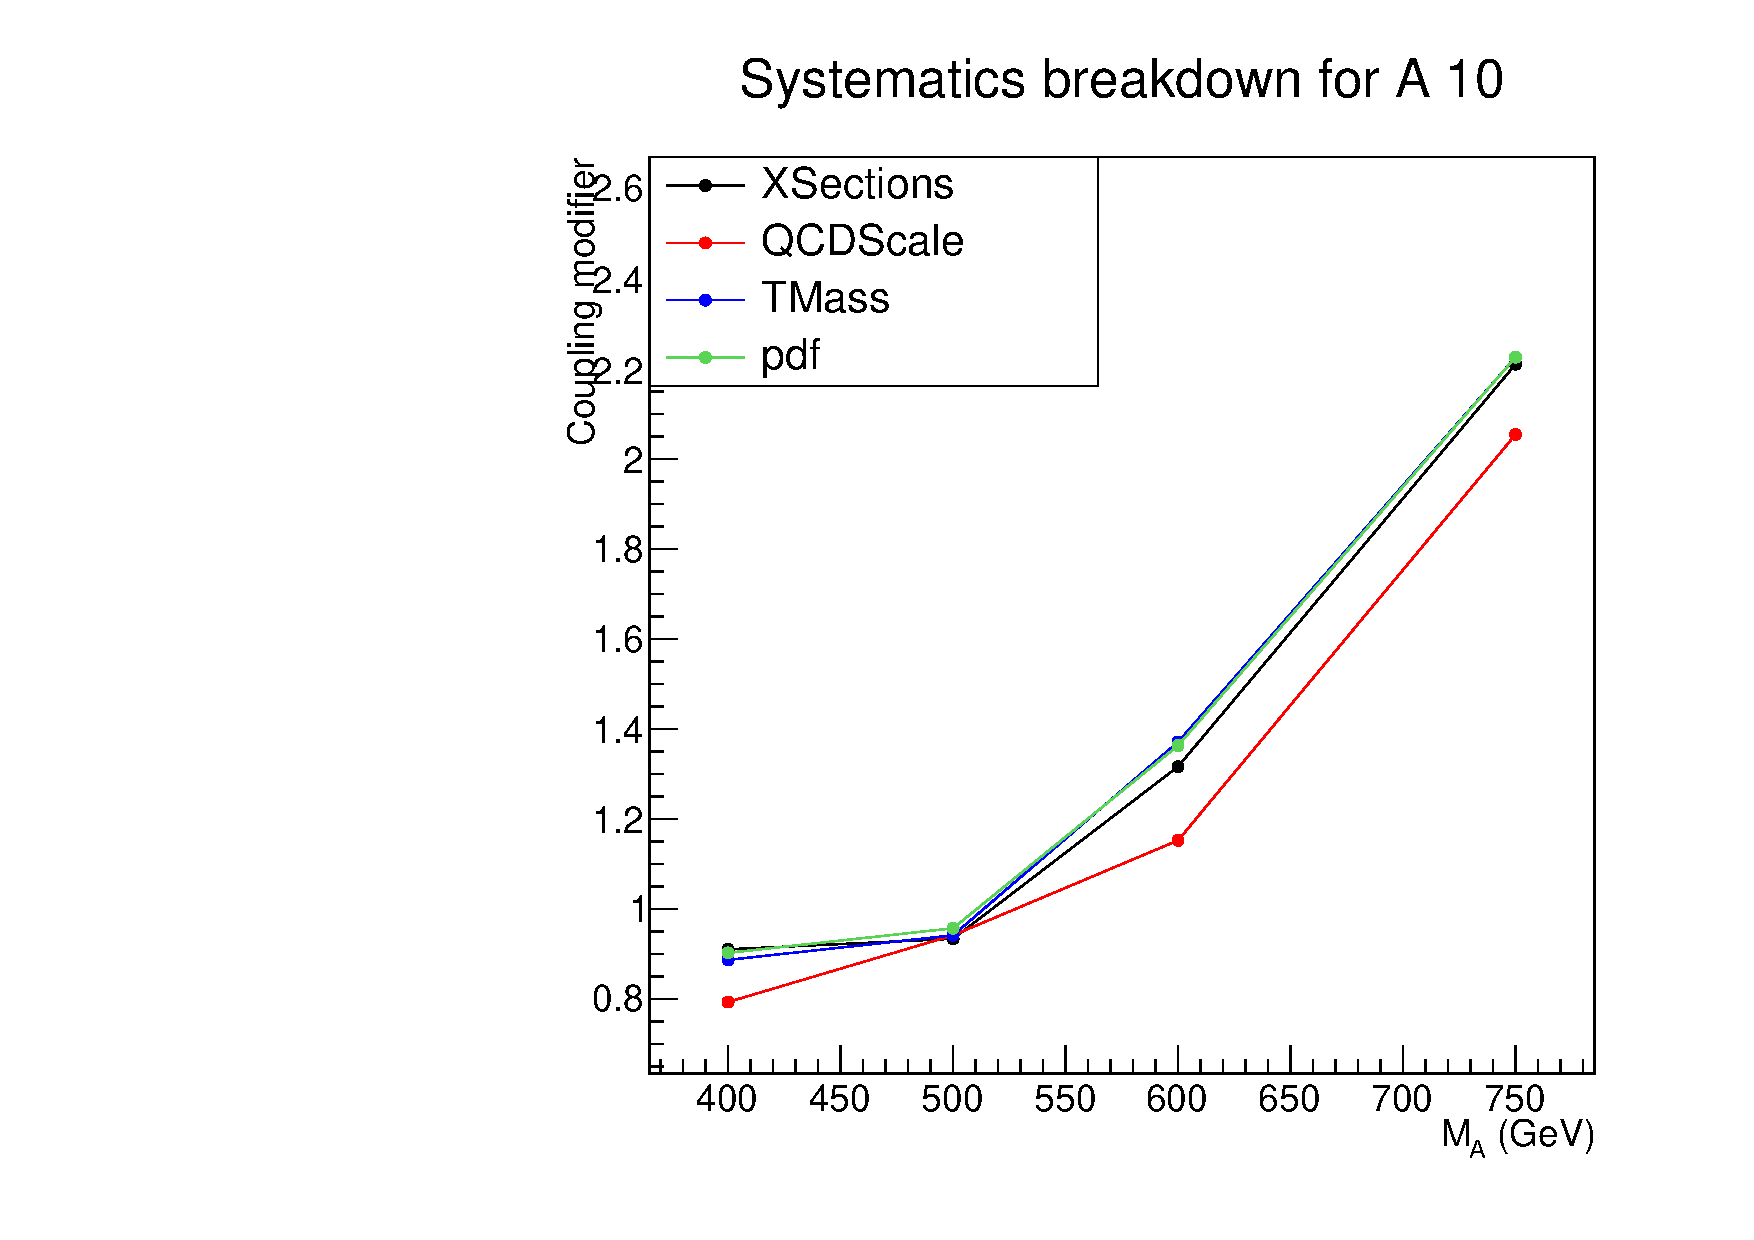
\includegraphics[width=0.35\textwidth,keepaspectratio=true]{fig/app5/breakdowns/theory_breakdown_A_10.pdf}
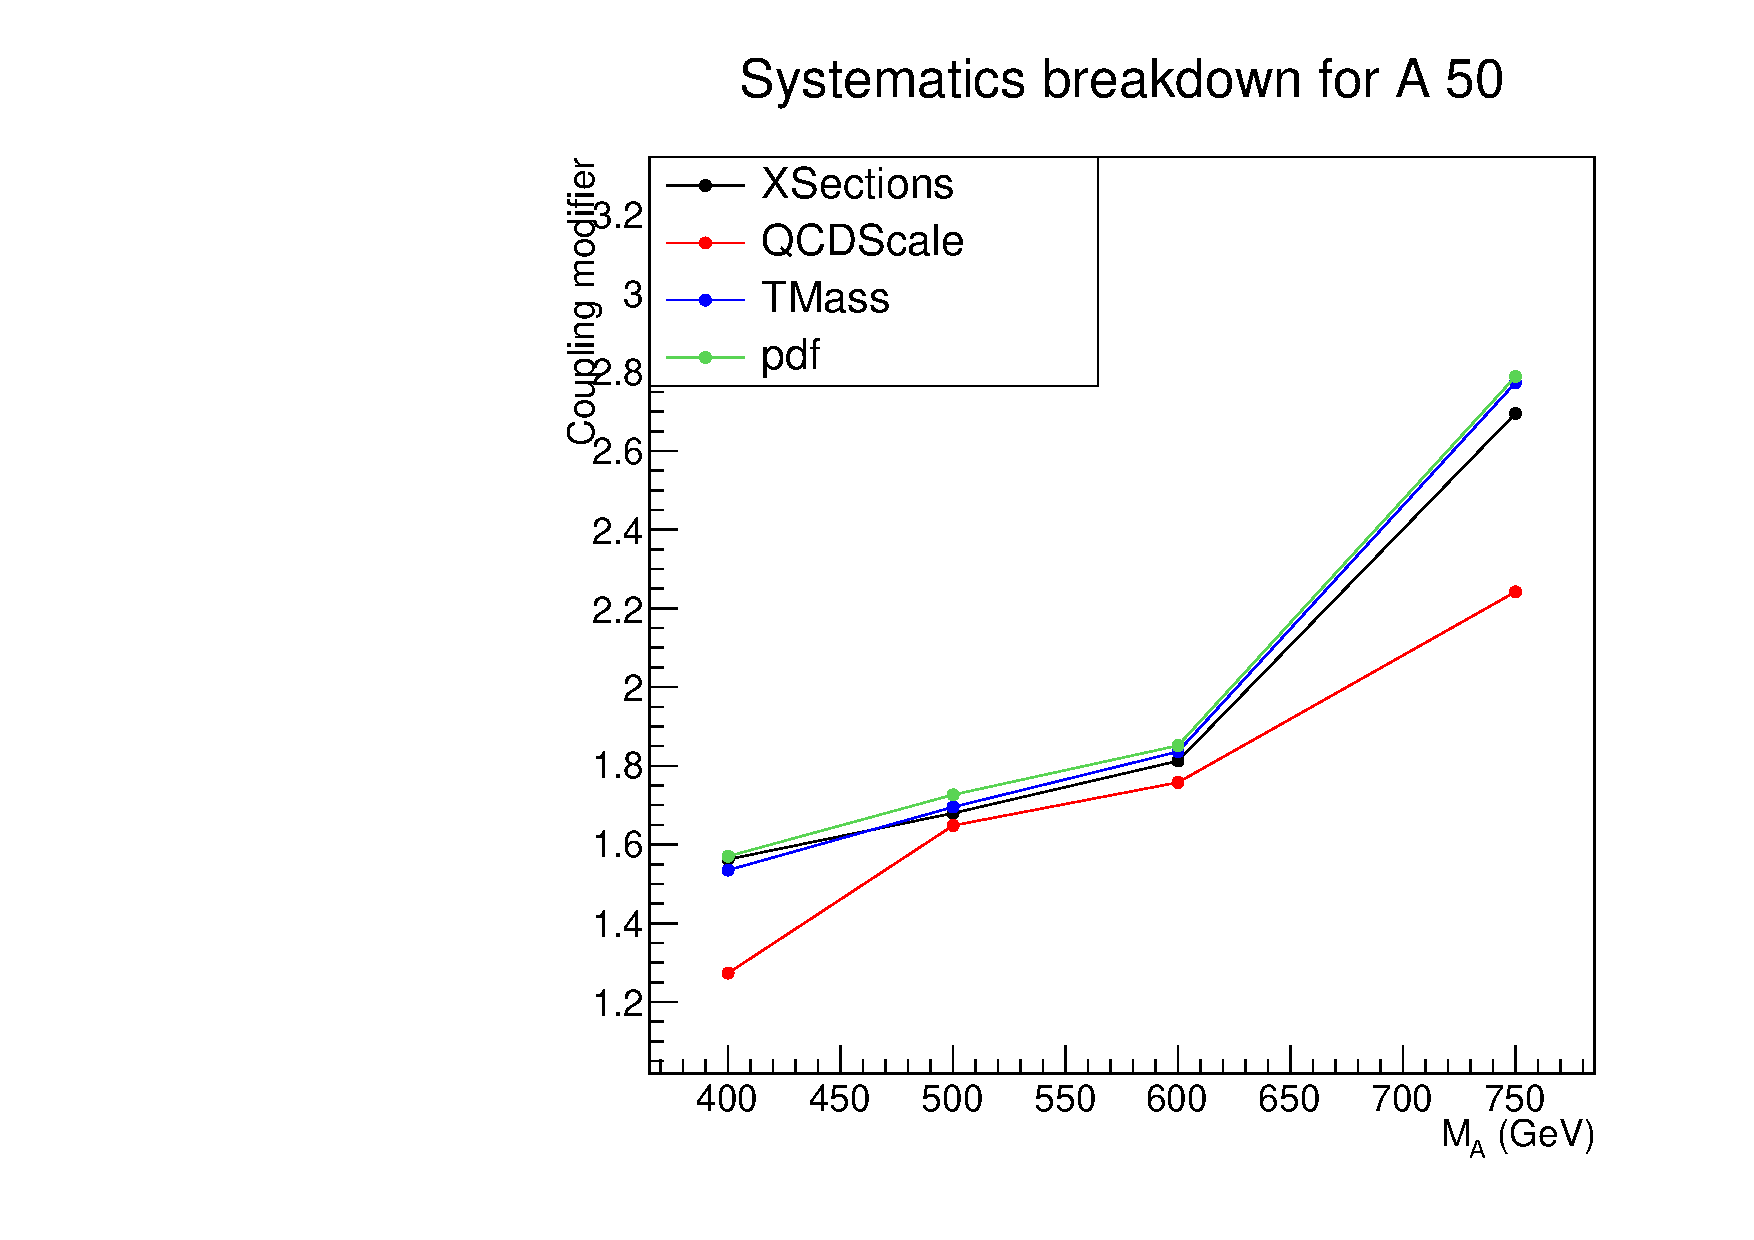
\includegraphics[width=0.35\textwidth,keepaspectratio=true]{fig/app5/breakdowns/theory_breakdown_A_50.pdf}
\caption{Expected upper limits on the coupling modifier with different groups of theory-related systematic uncertainties removed. The nominal limits are shown as the blue curve. The expected upper limits are shown for pseudoscalar signal as a function of mass for different values of the relative width, ranging from 2.5 to 50\%.}
\label{fig:theory_breakdown_awidths}
\end{figure}

\begin{figure}[!Hhtb]
\centering
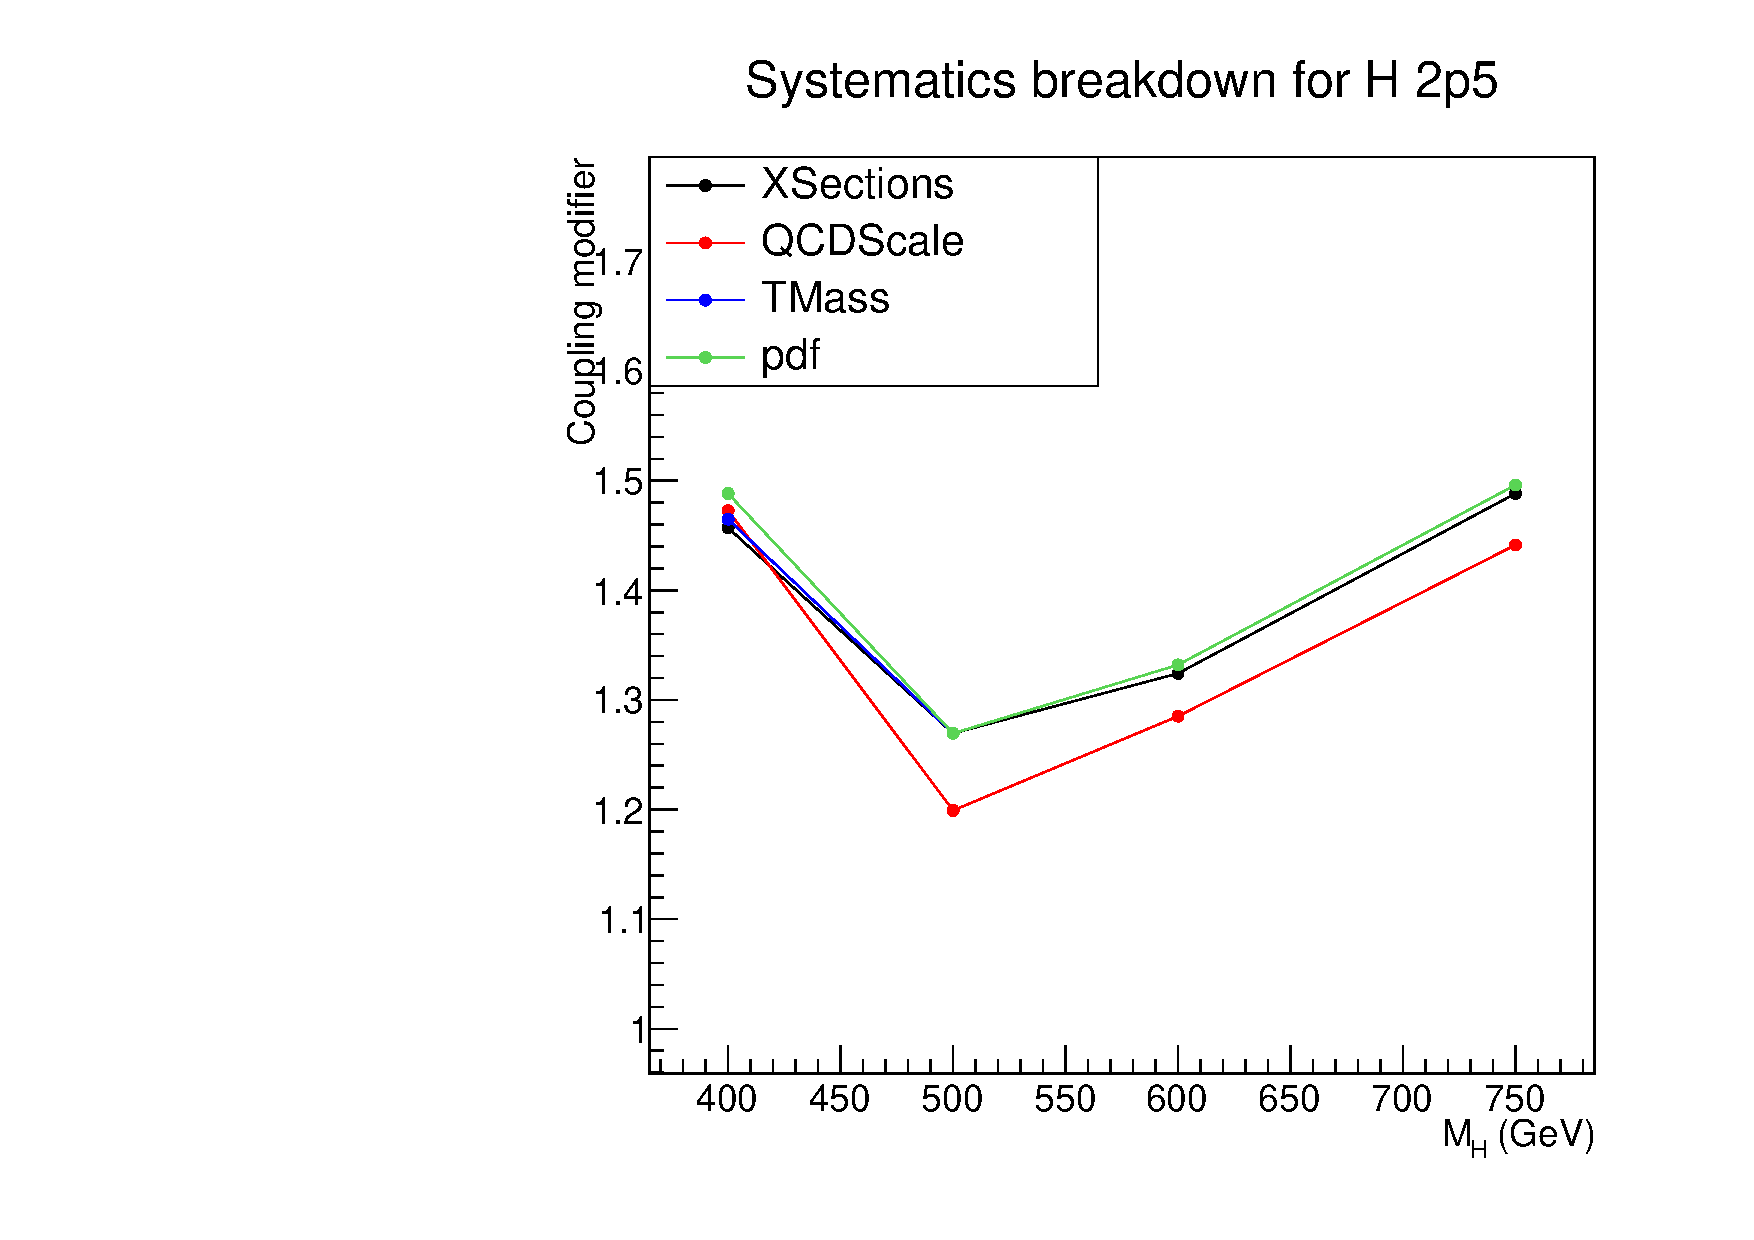
\includegraphics[width=0.35\textwidth,keepaspectratio=true]{fig/app5/breakdowns/theory_breakdown_H_2p5.pdf}
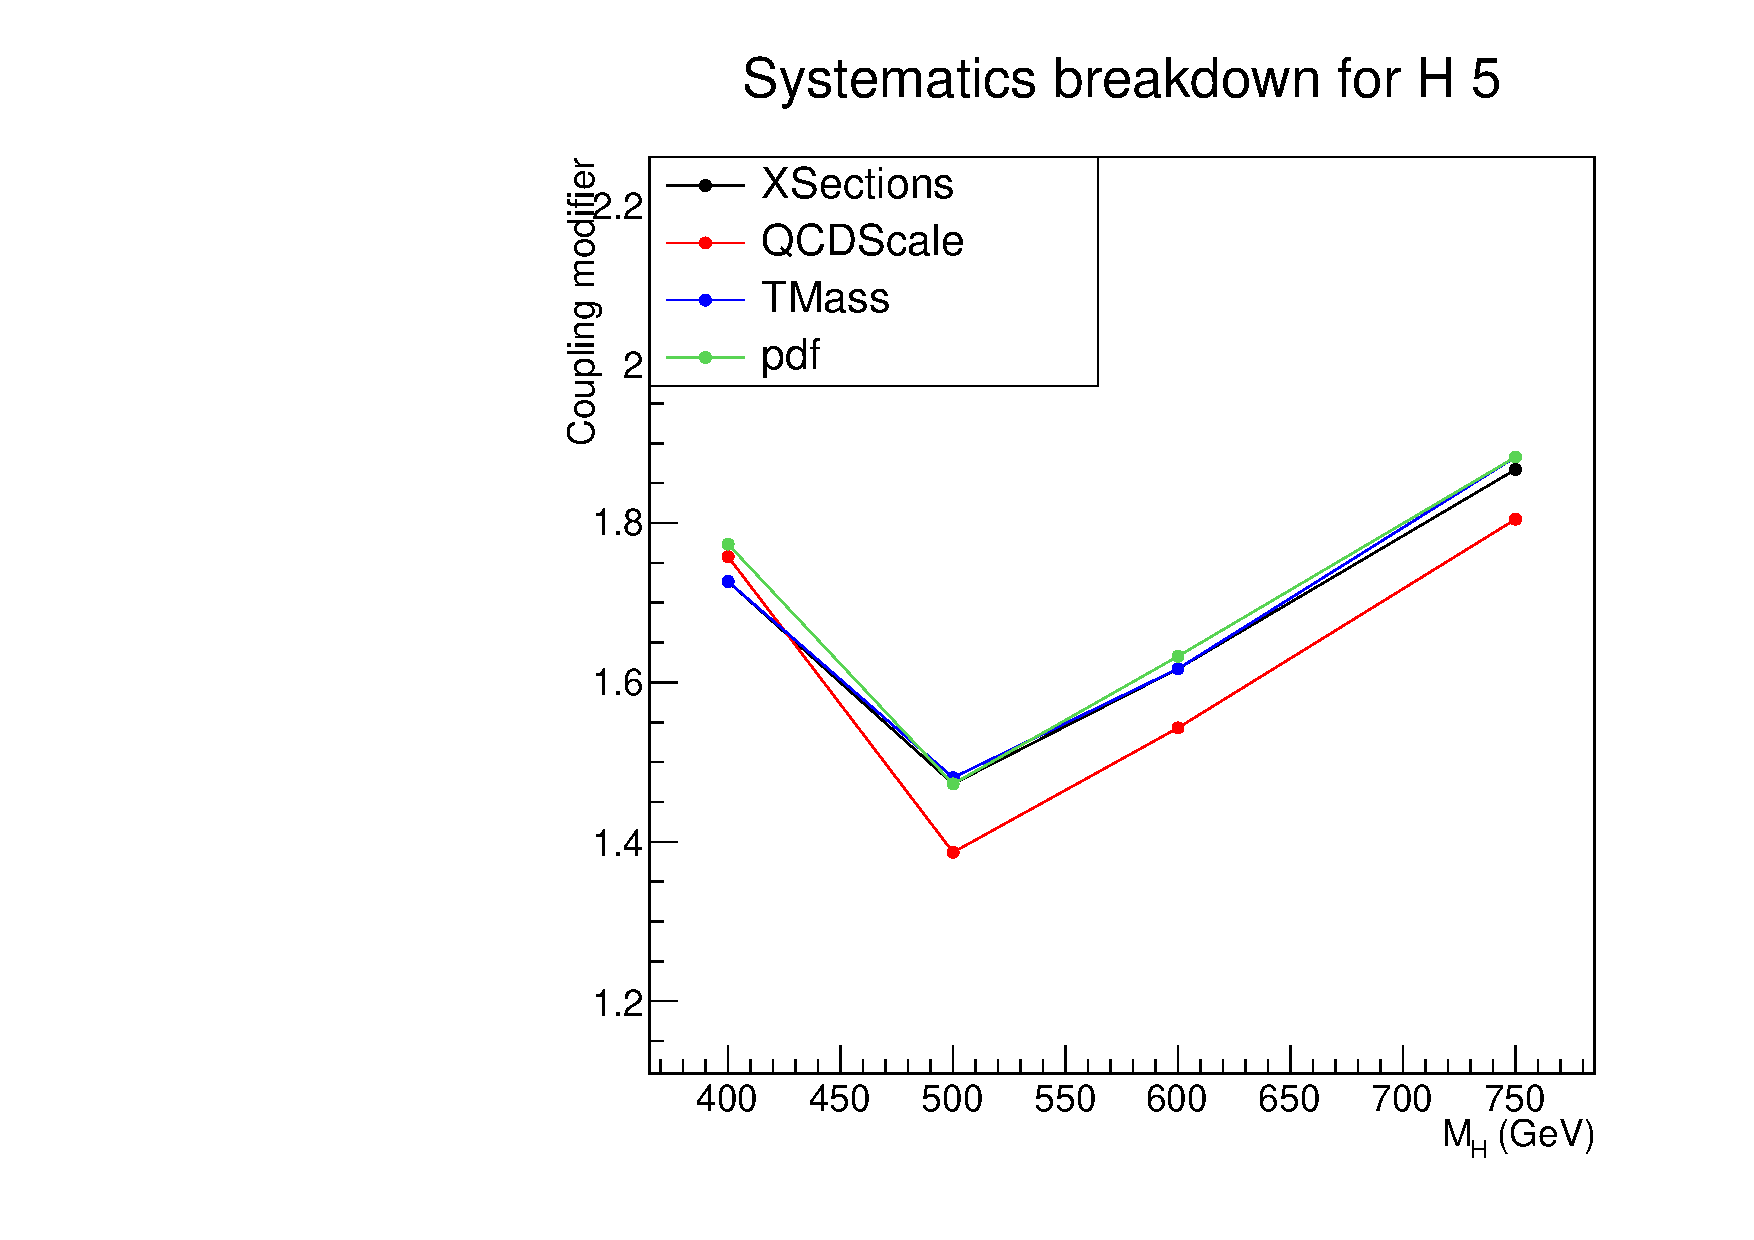
\includegraphics[width=0.35\textwidth,keepaspectratio=true]{fig/app5/breakdowns/theory_breakdown_H_5.pdf}
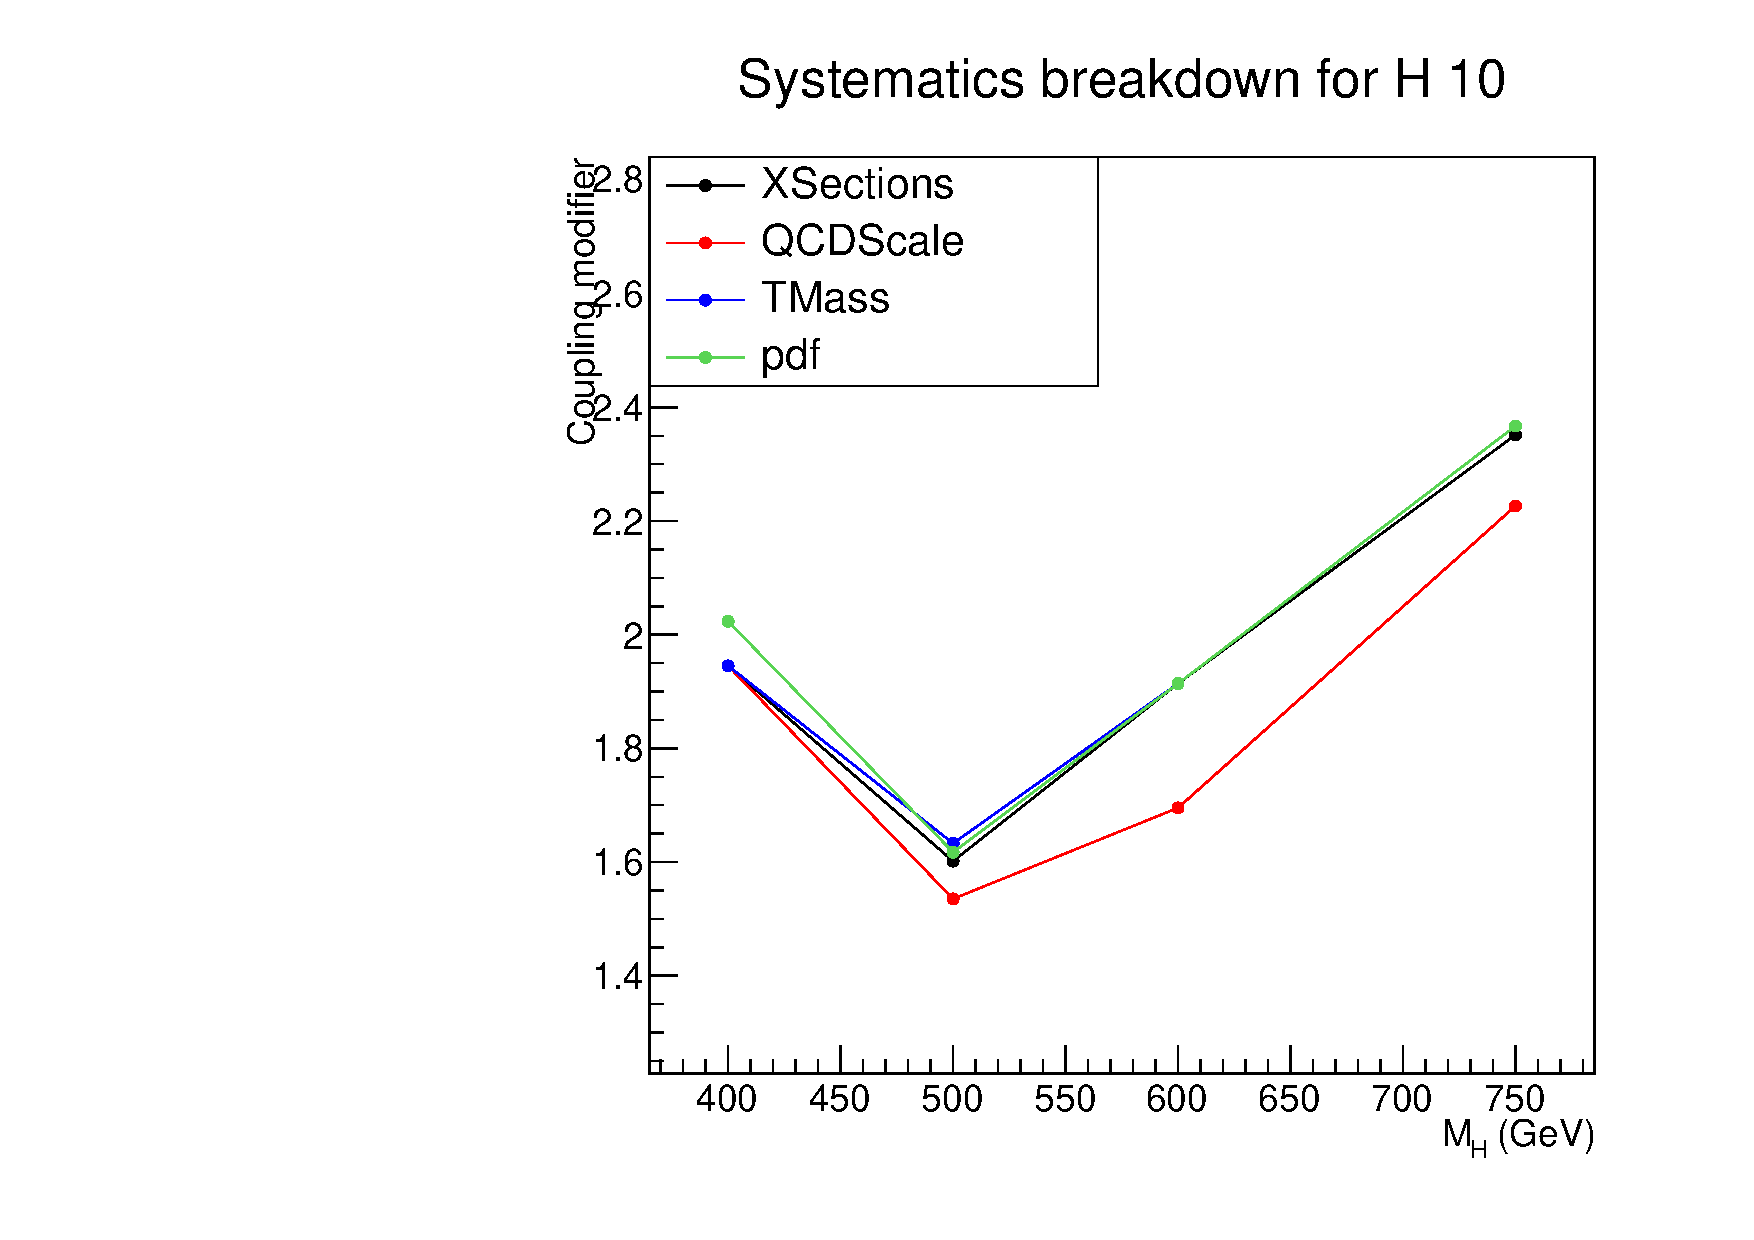
\includegraphics[width=0.35\textwidth,keepaspectratio=true]{fig/app5/breakdowns/theory_breakdown_H_10.pdf}
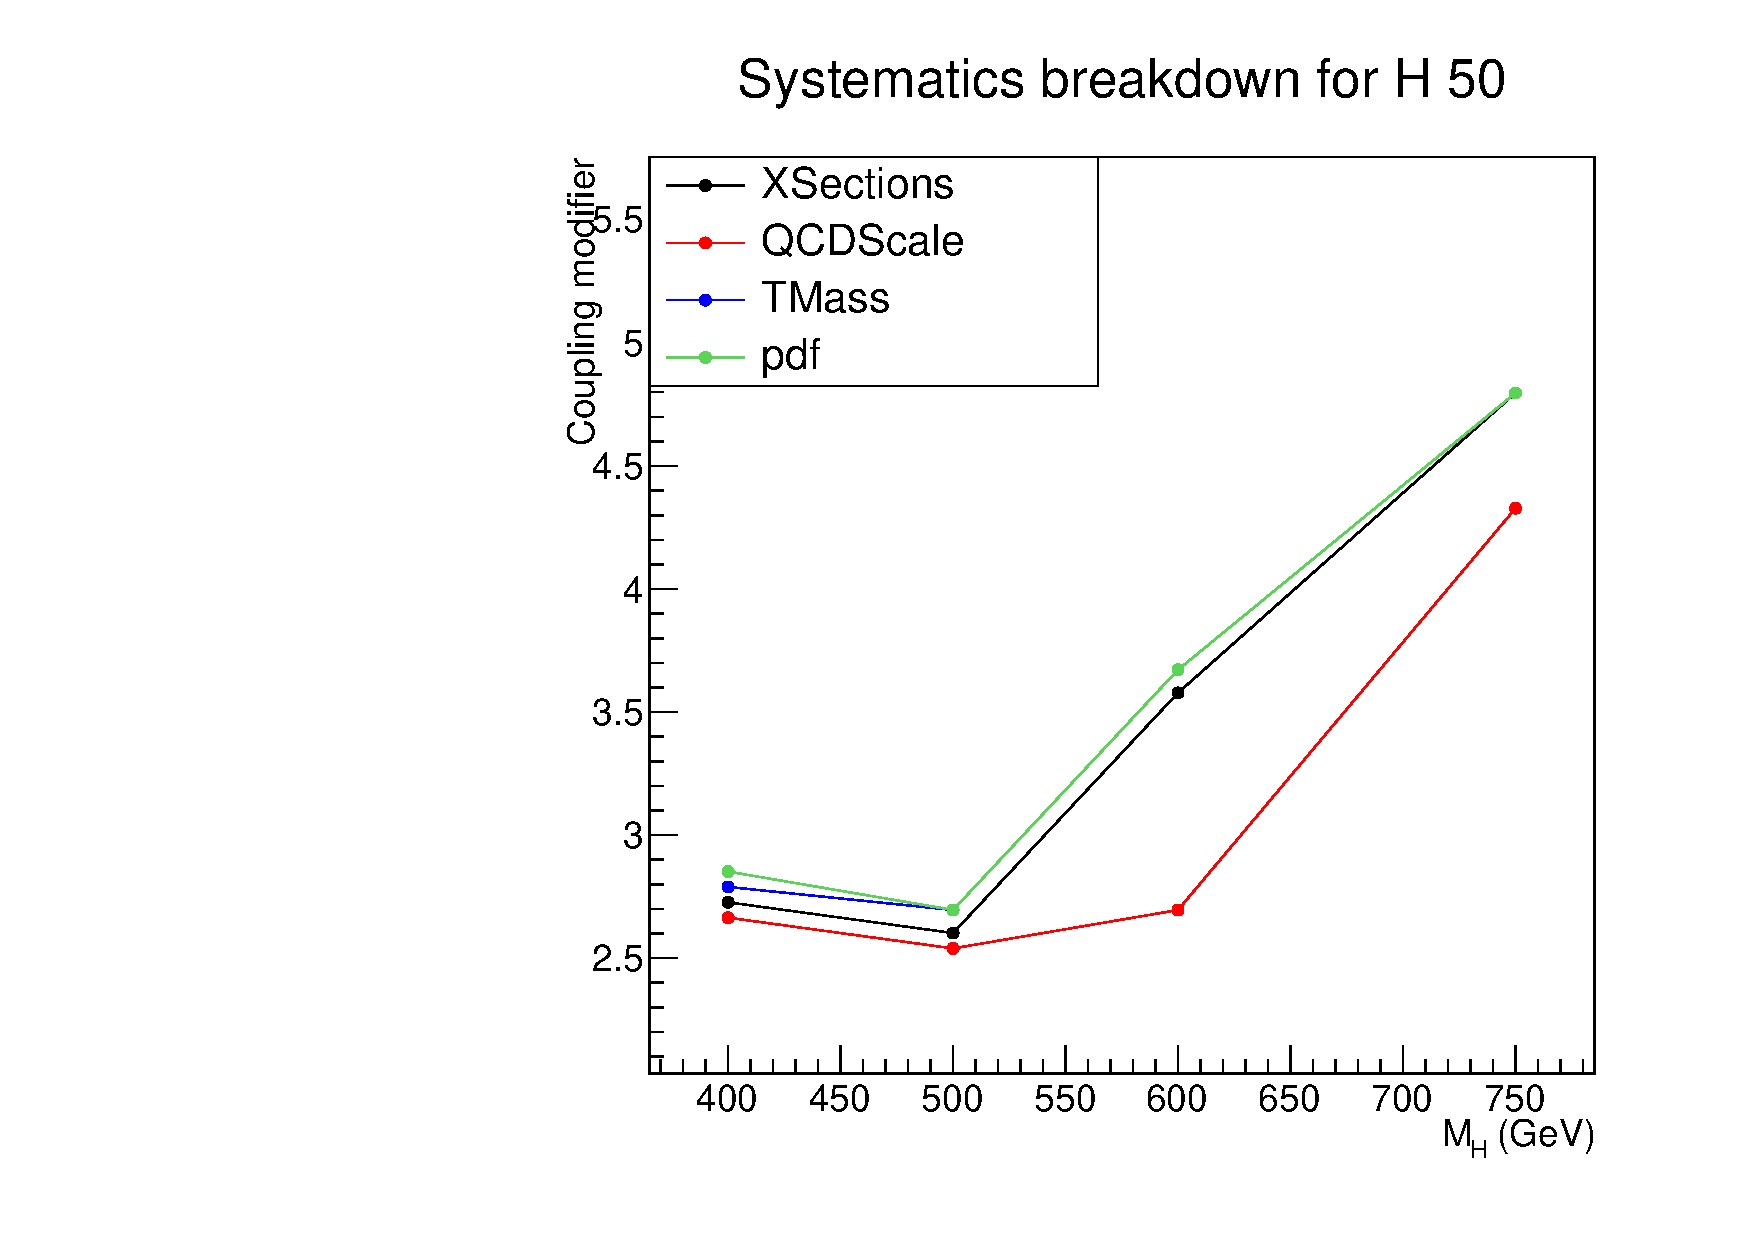
\includegraphics[width=0.35\textwidth,keepaspectratio=true]{fig/app5/breakdowns/theory_breakdown_H_50.pdf}
\caption{Expected upper limits on the coupling modifier with different groups of theory-related systematic uncertainties removed. The nominal limits are shown as the blue curve. The expected upper limits are shown for scalar signal as a function of mass for different values of the relative width, ranging from 2.5 to 50\%.}
\label{fig:theory_breakdown_hwidths}
\end{figure}

\begin{figure}[!Hhtb]
\centering
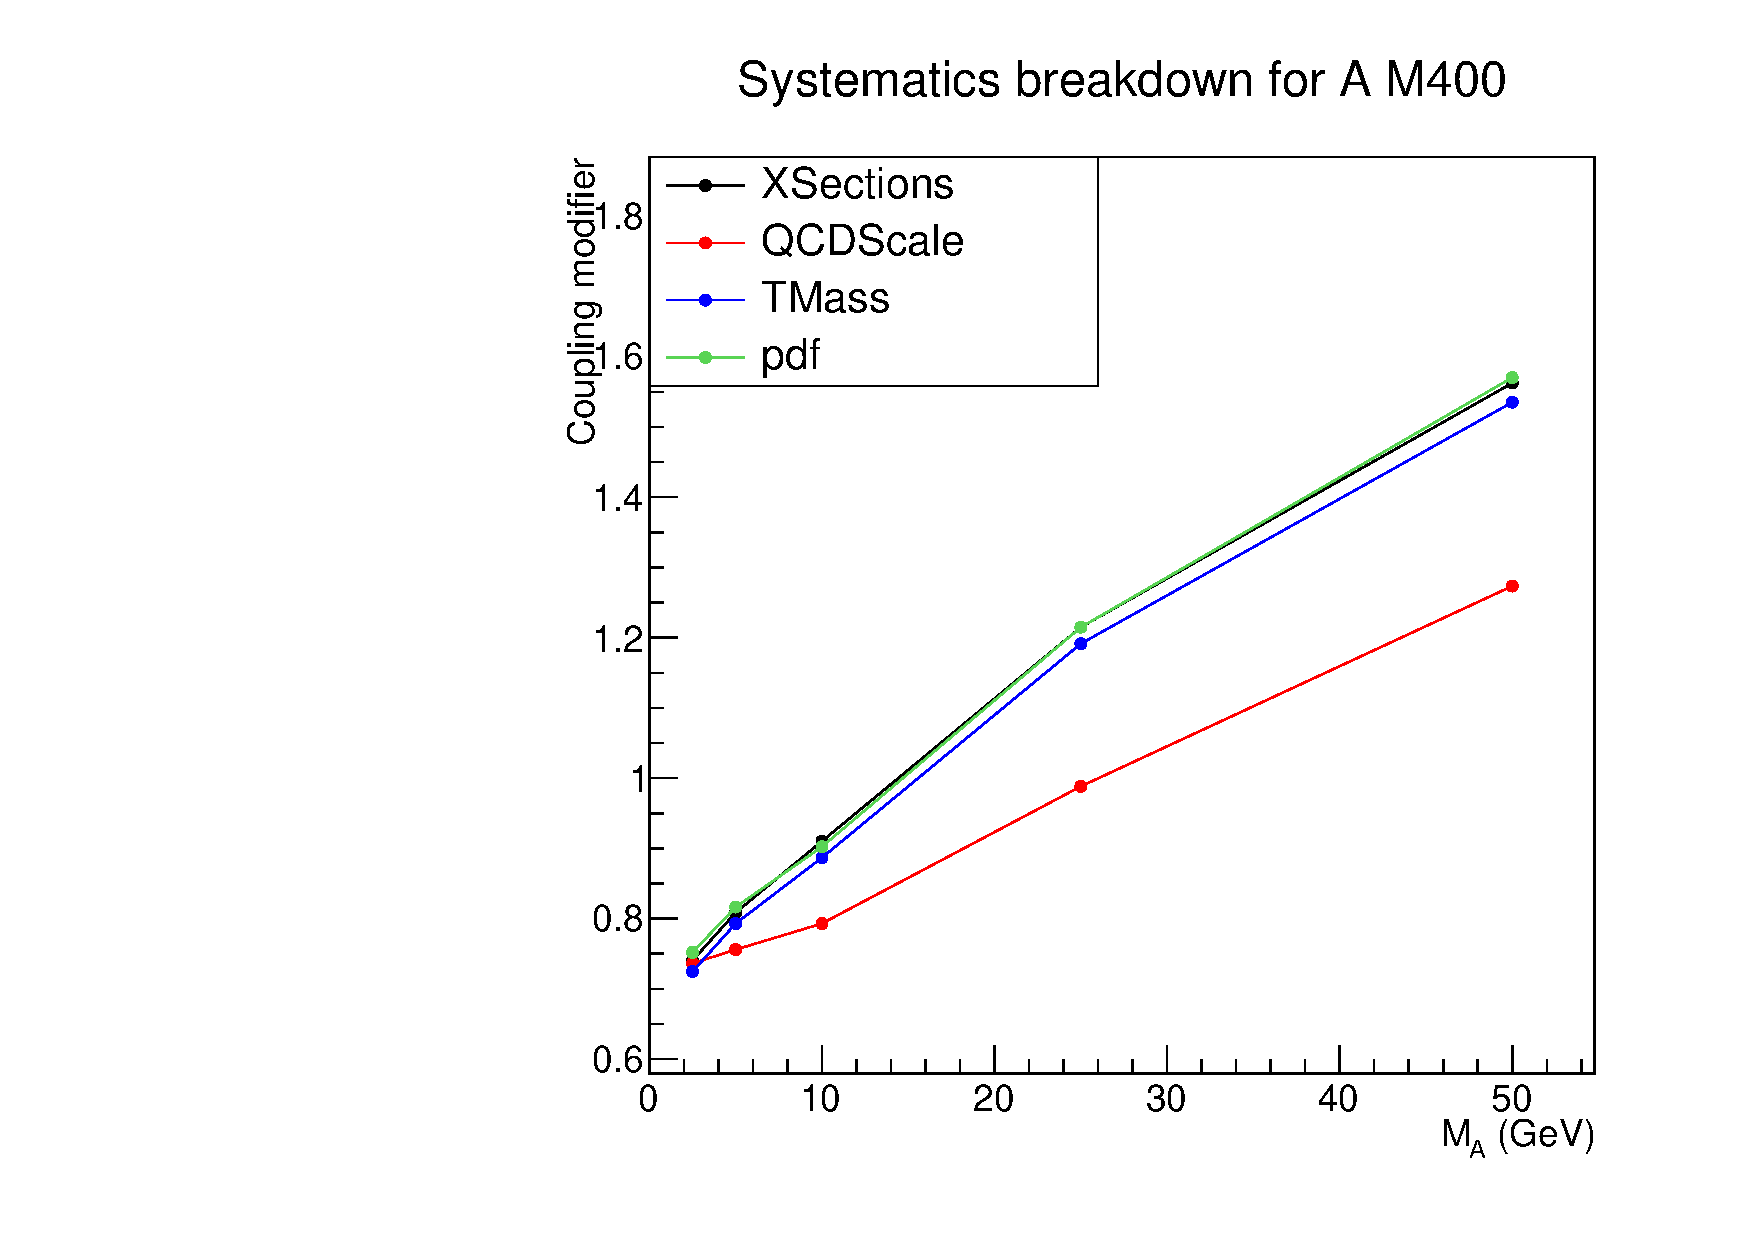
\includegraphics[width=0.35\textwidth,keepaspectratio=true]{fig/app5/breakdowns/theory_breakdown_A_M400.pdf}
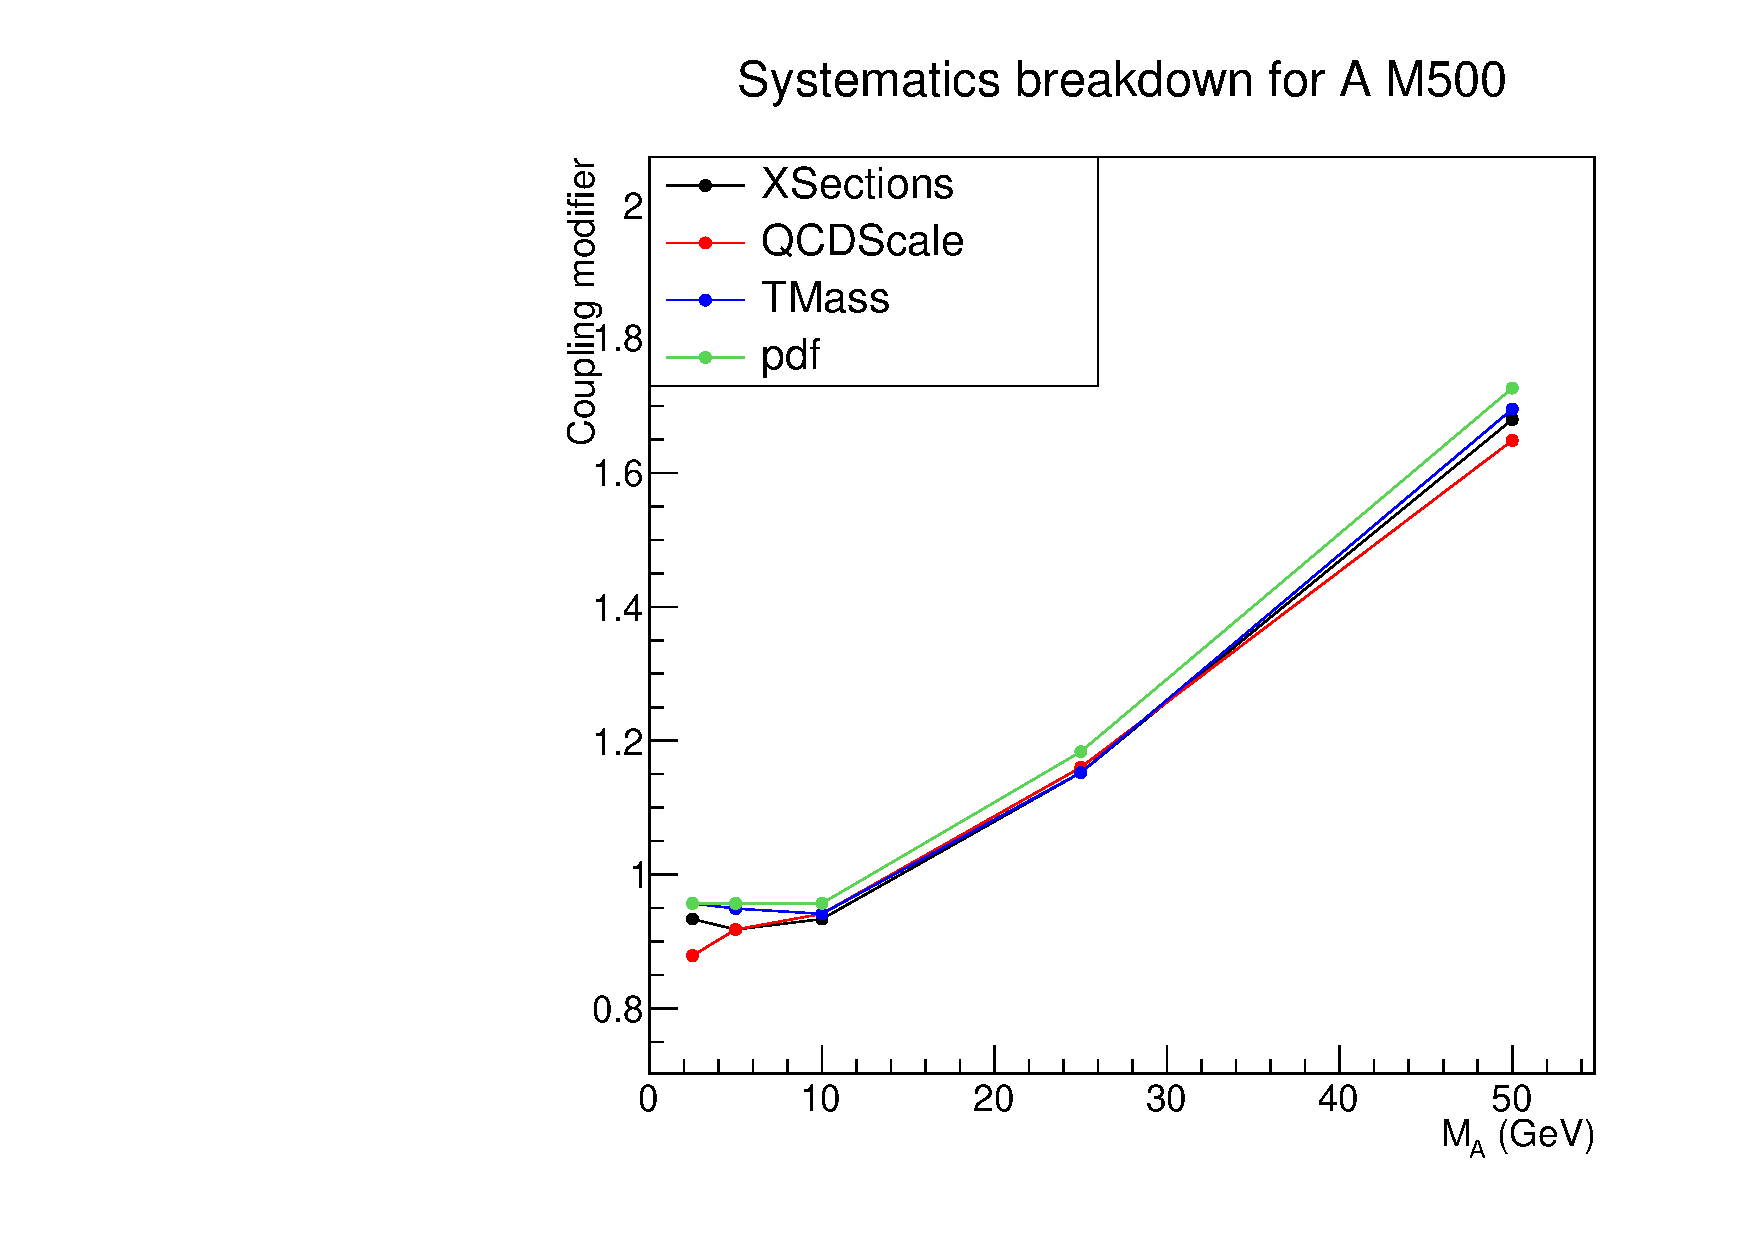
\includegraphics[width=0.35\textwidth,keepaspectratio=true]{fig/app5/breakdowns/theory_breakdown_A_M500.pdf}
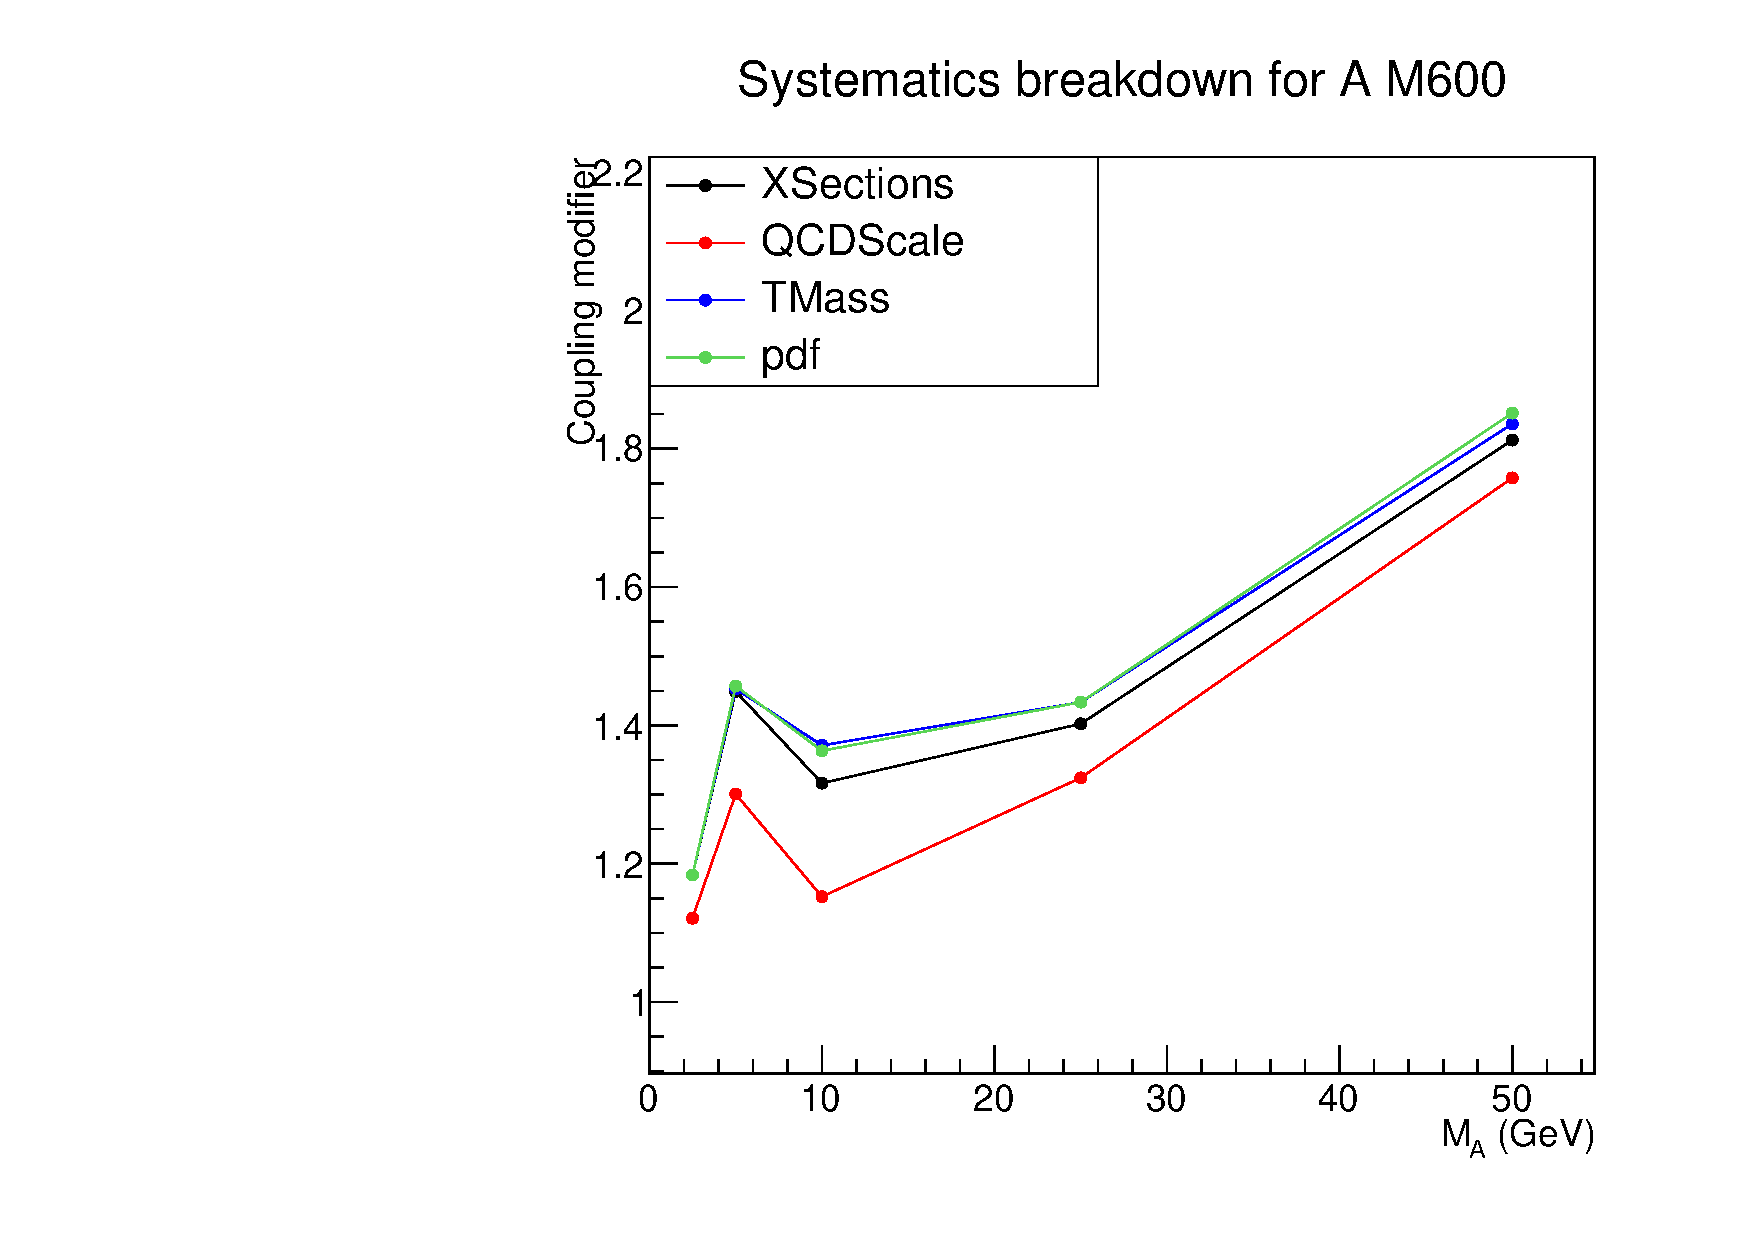
\includegraphics[width=0.35\textwidth,keepaspectratio=true]{fig/app5/breakdowns/theory_breakdown_A_M600.pdf}
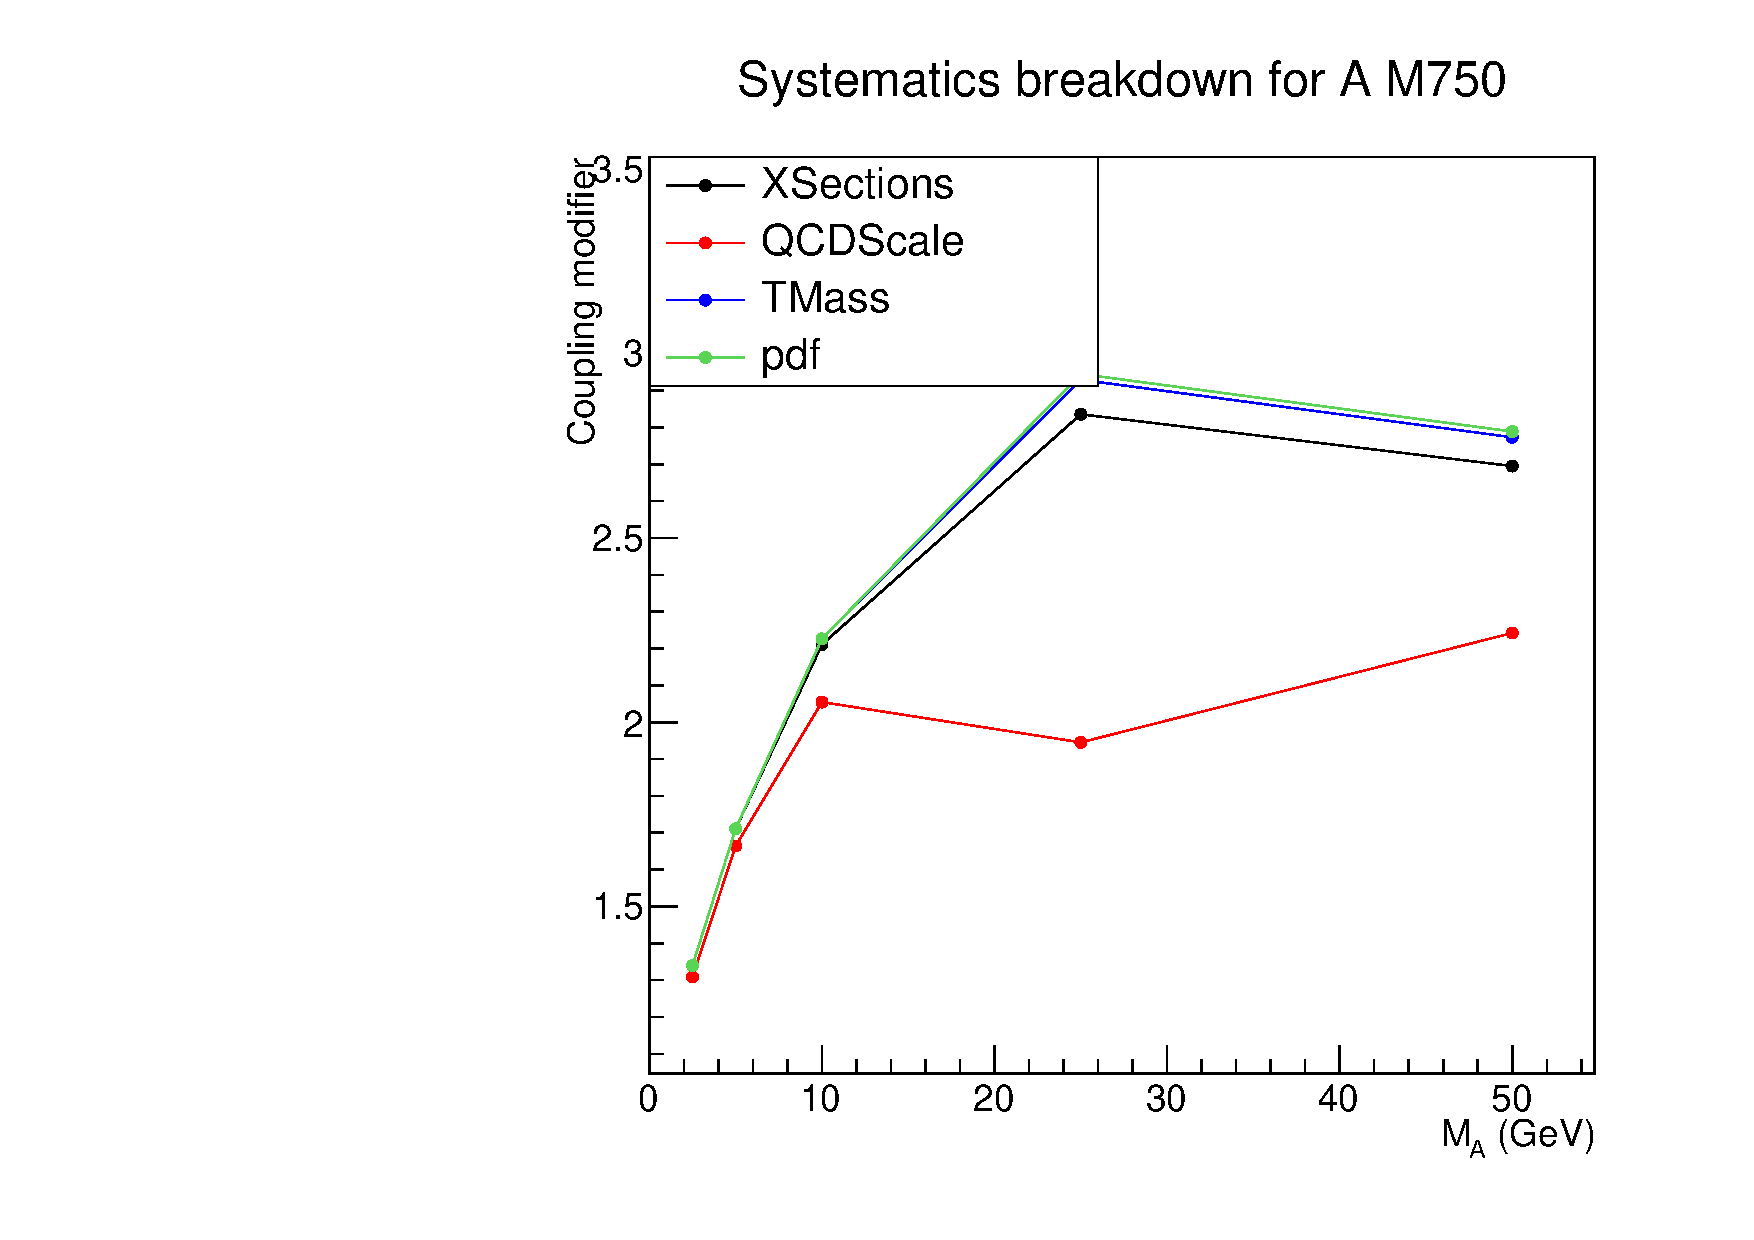
\includegraphics[width=0.35\textwidth,keepaspectratio=true]{fig/app5/breakdowns/theory_breakdown_A_M750.pdf}
\caption{Expected upper limits on the coupling modifier with different groups of theory-related systematic uncertainties removed. The nominal limits are shown as the blue curve. The expected upper limits are shown for pseudoscalar signal as a function of relative width for different values of the mass, ranging from 400 to 750~GeV.}
\label{fig:theory_breakdown_amass}
\end{figure}



\begin{figure}[!Hhtb]
\centering
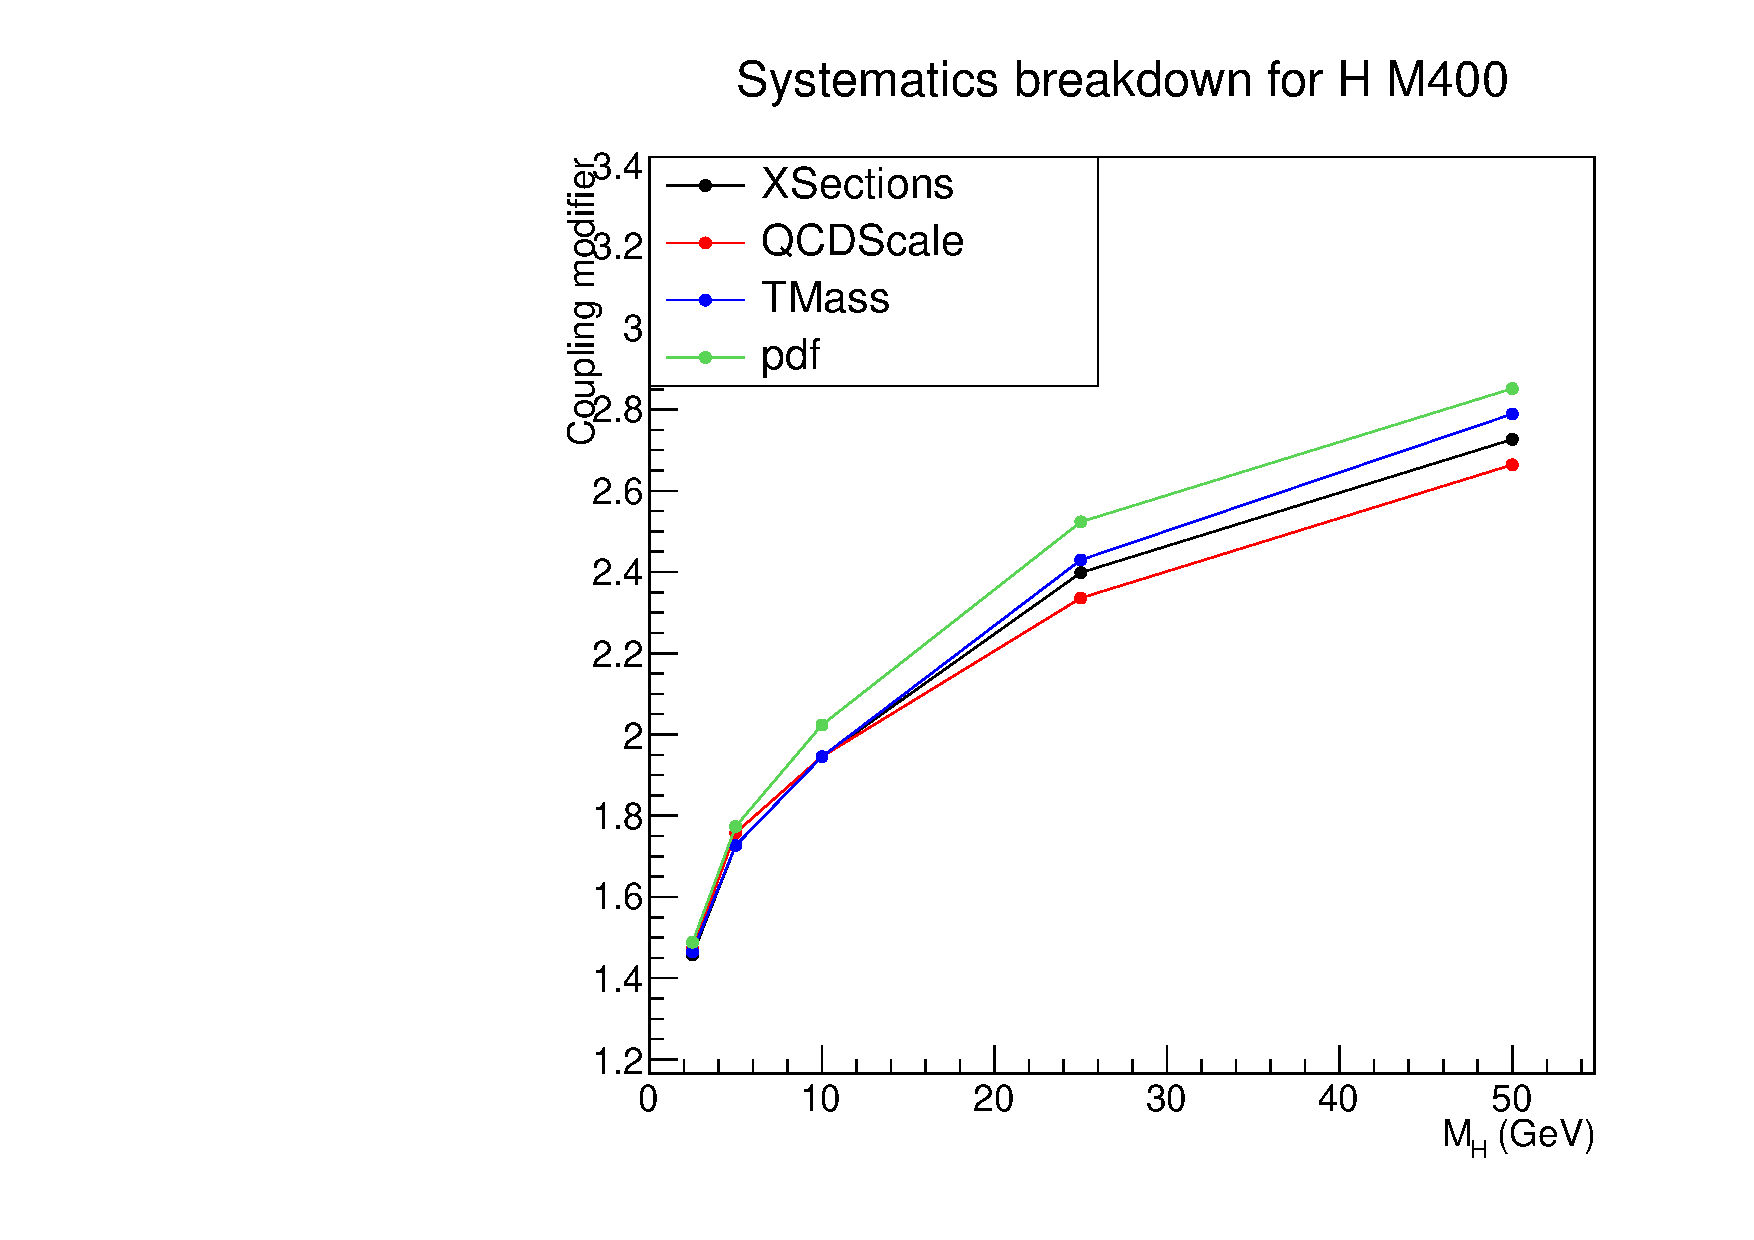
\includegraphics[width=0.35\textwidth,keepaspectratio=true]{fig/app5/breakdowns/theory_breakdown_H_M400.pdf}
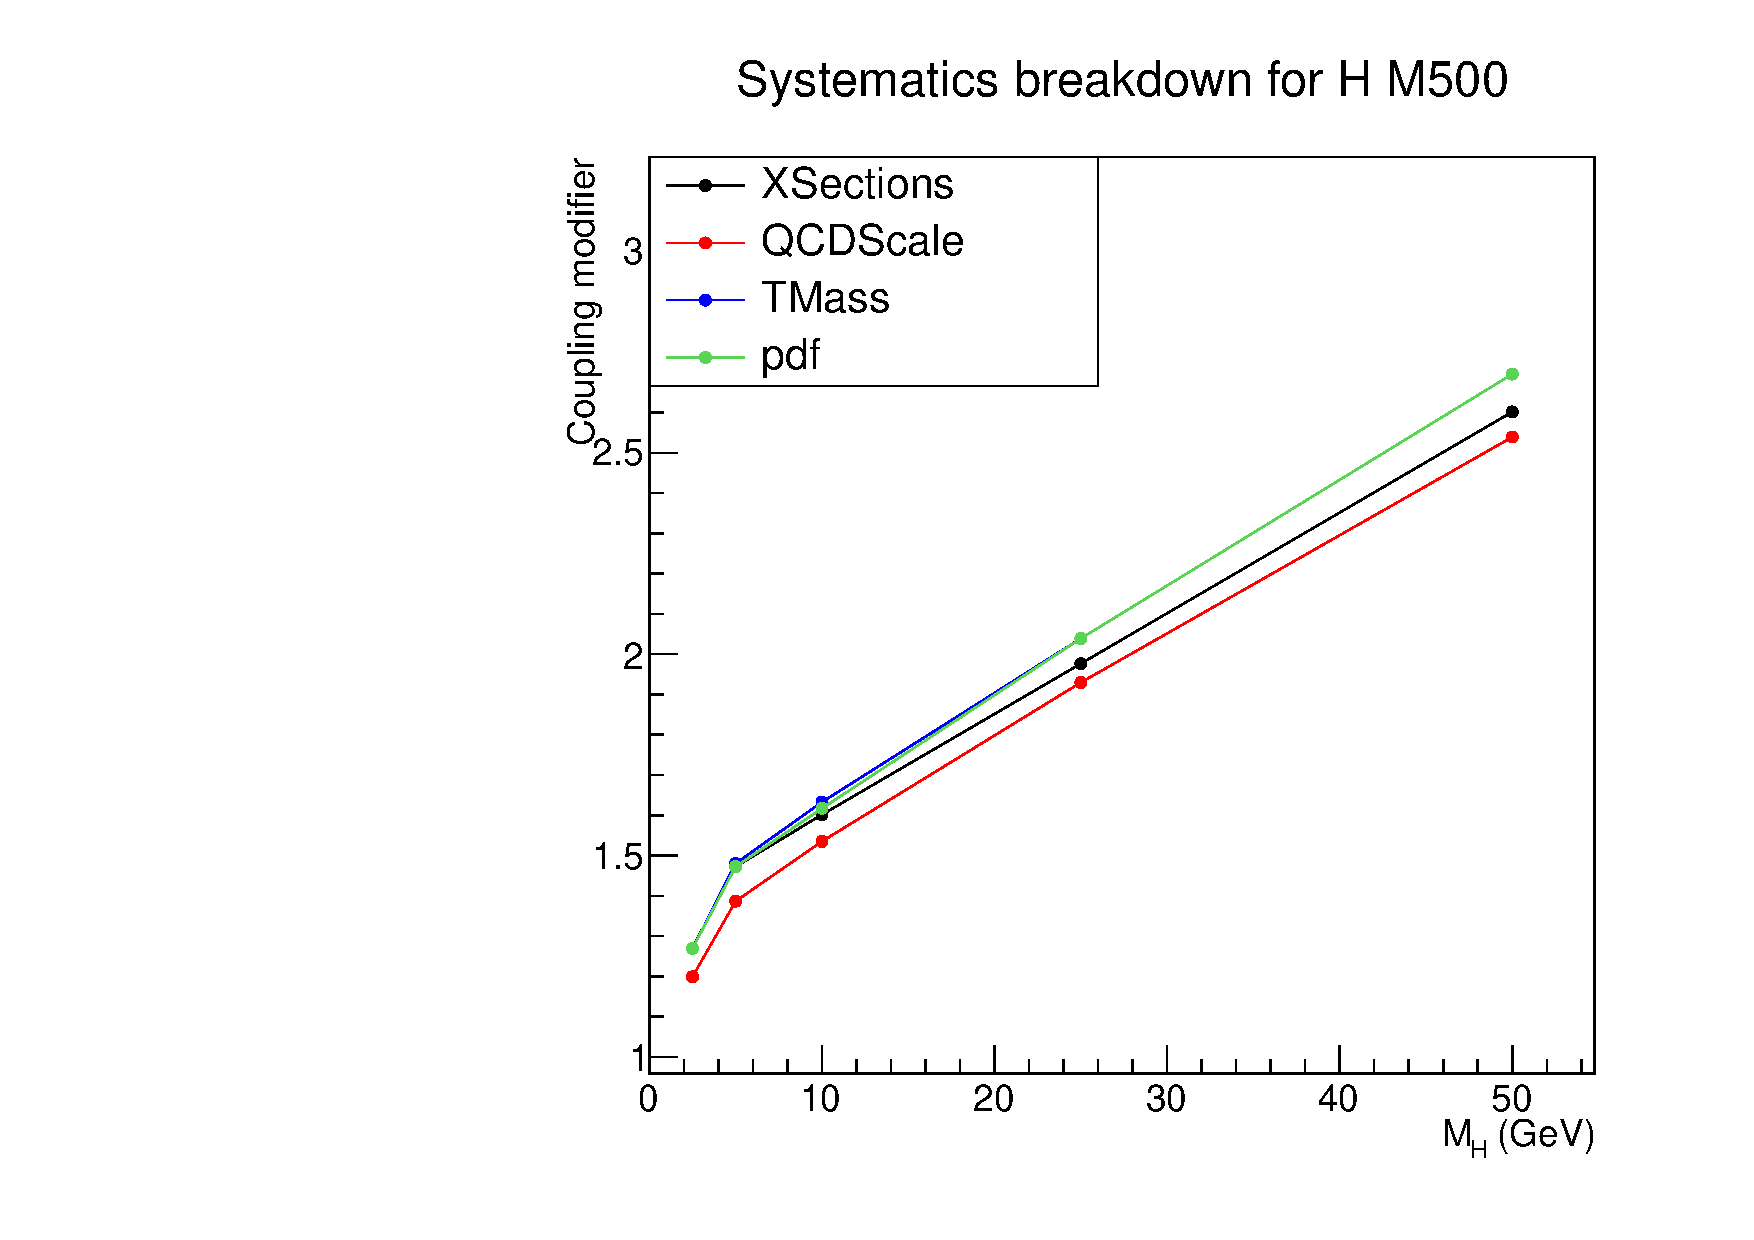
\includegraphics[width=0.35\textwidth,keepaspectratio=true]{fig/app5/breakdowns/theory_breakdown_H_M500.pdf}
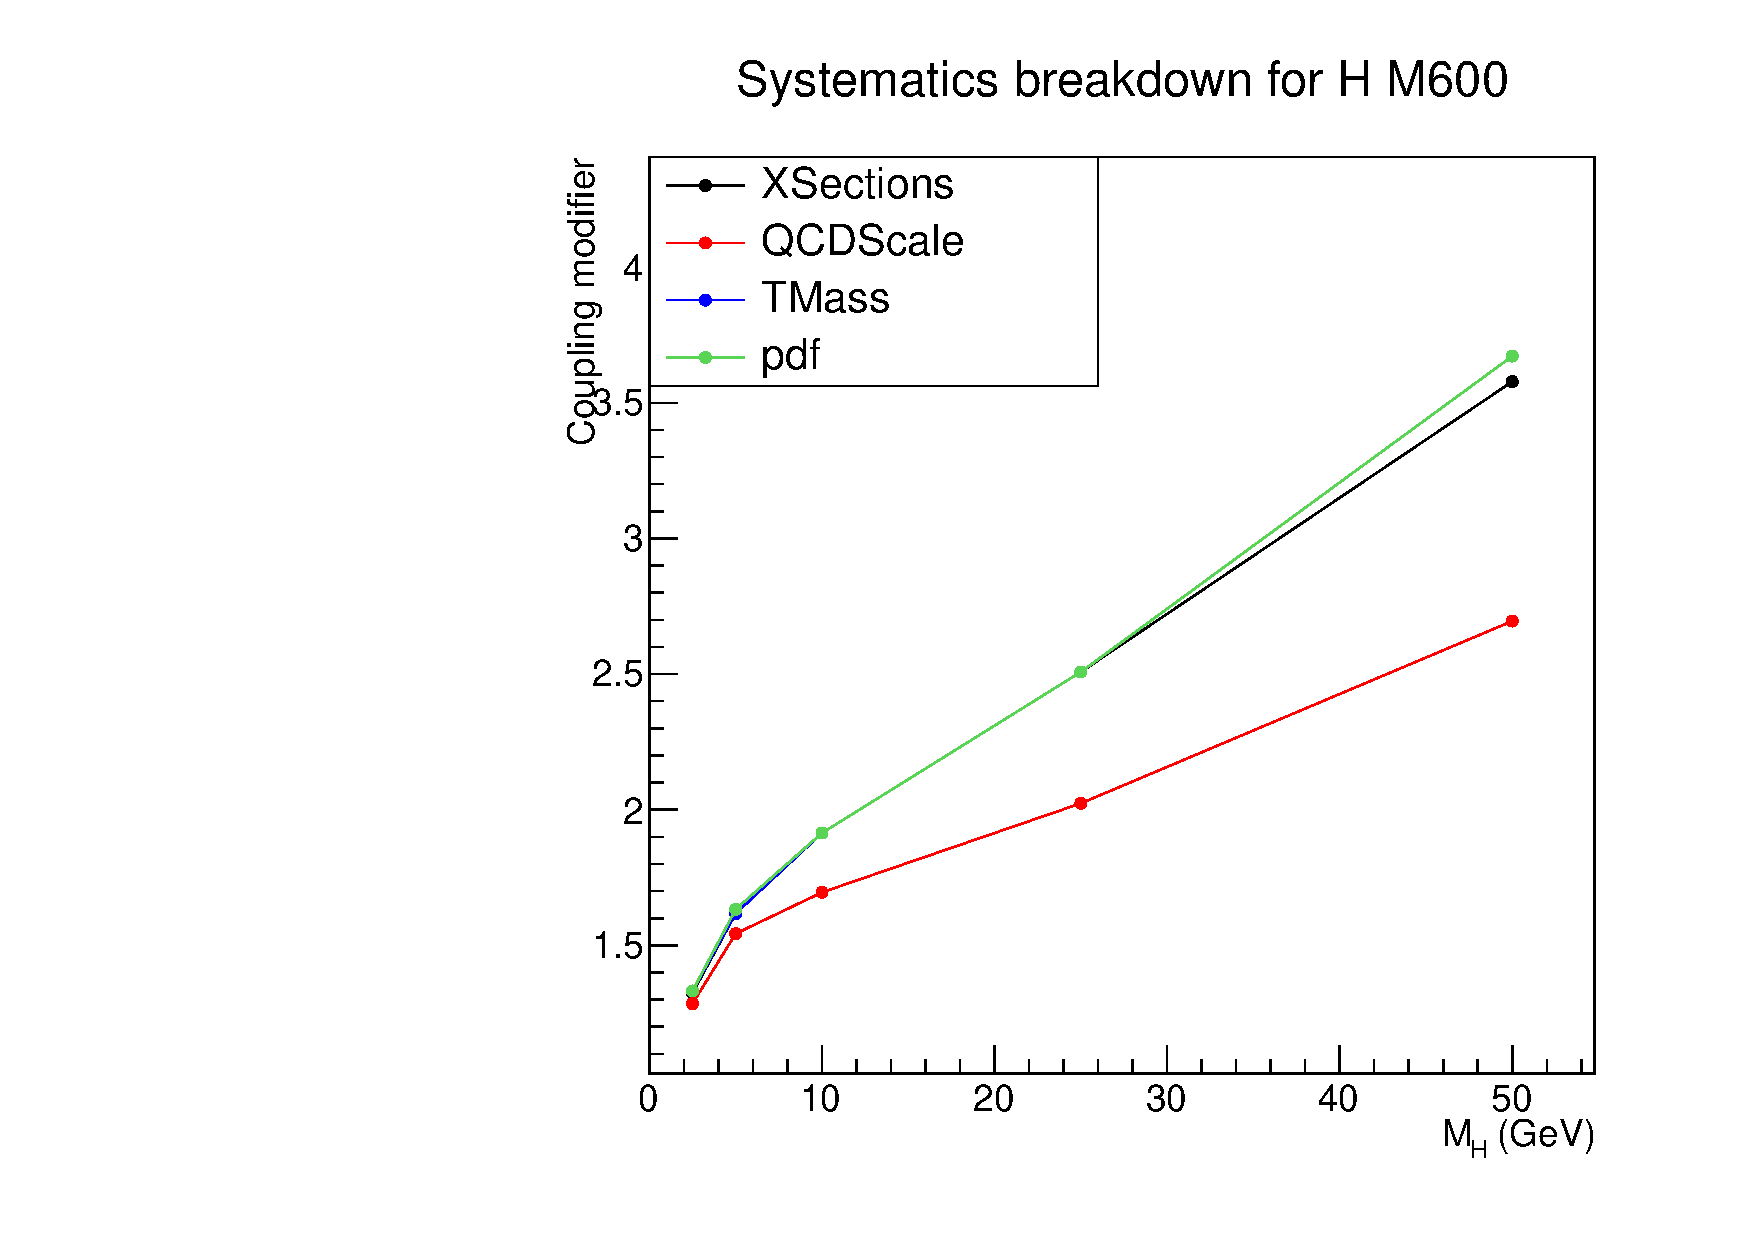
\includegraphics[width=0.35\textwidth,keepaspectratio=true]{fig/app5/breakdowns/theory_breakdown_H_M600.pdf}
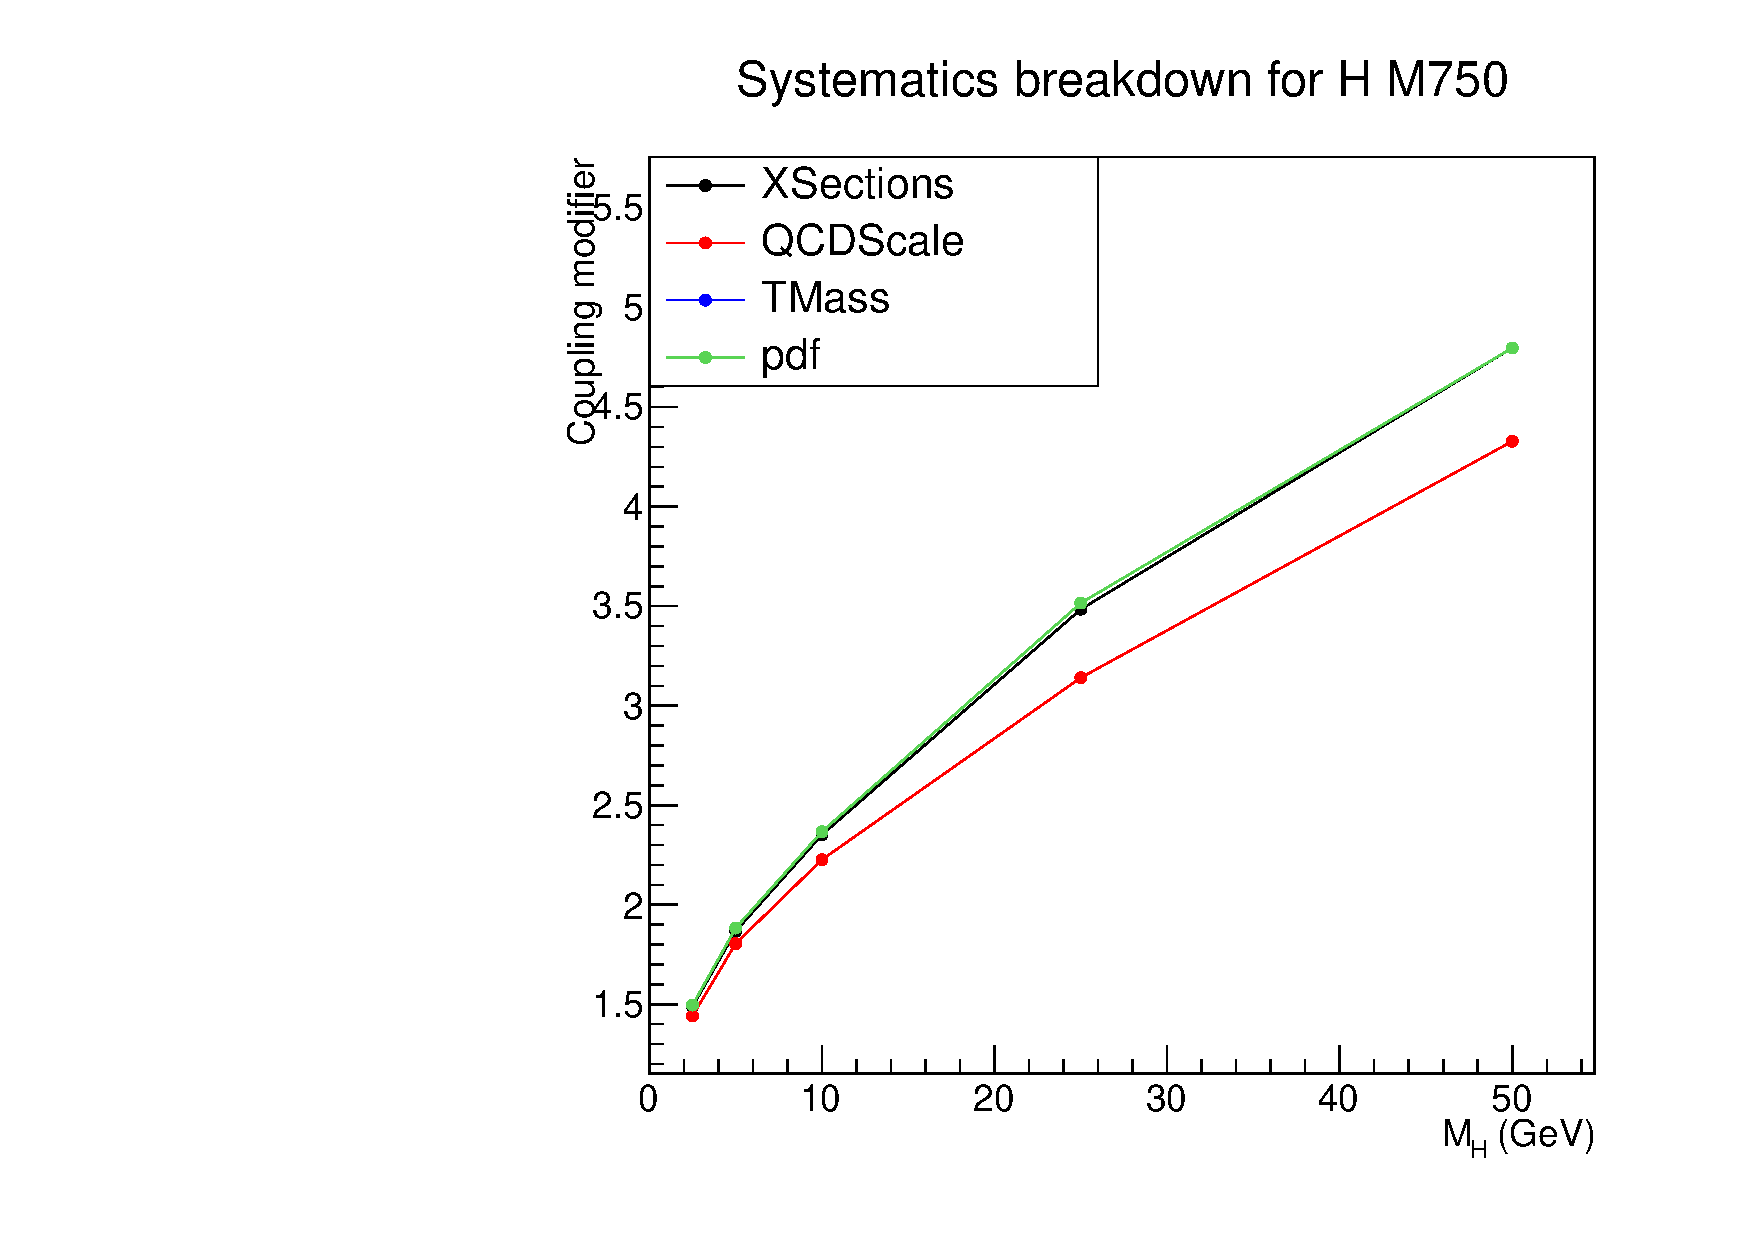
\includegraphics[width=0.35\textwidth,keepaspectratio=true]{fig/app5/breakdowns/theory_breakdown_H_M750.pdf}
\caption{Expected upper limits on the coupling modifier with different groups of theory-related systematic uncertainties removed. The nominal limits are shown as the blue curve. The expected upper limits are shown for pseudoscalar signal as a function of relative width for different values of the mass, ranging from 400 to 750~GeV.}
\label{fig:theory_breakdown_hmass}
\end{figure}

The results presented in this section answer the question ``How would the expected limits change if certain groups of systematic uncertainties were irrelevant?'', which can also be understood as the impact the according systematic uncertainties have on the values of the expected upper limits on the coupling strength.
Figures~\ref{fig:breakdown_awidths}-\ref{fig:breakdown_hmass} show the upper limits with either experimental, theoretical cross sections, other theory-related, or bin-by-bin uncertainties removed.
Uncertainties in the cross sections of background process have a negligible overall impact, and experimental uncertainties also have a minor overall impact.
However, both the expected upper limits with bin-by-bin uncertainties and the other theory-related uncertainties removed show a significant improvement with respect to the nominal upper limits.
For higher widths, the theory-related uncertainties become yet more important.

To understand the impact of the theory-related uncertainties in more detail, figures~\ref{fig:theory_breakdown_awidths}-\ref{fig:theory_breakdown_hmass} show the combined impacts of cross-section related uncertainties, missing higher orders as obtained from scale variations, top quark mass, and PDF uncertainties.
For $m_\Phi = 400~GeV$ and low to moderate width, the top quark mass uncertainty has the largest impact, with very similar impacts from PDF uncertainties and the other two combined sources.
Starting from $m_\Phi = 500~GeV$, scale variations become most important, with all other combined sources giving similar additional contributions.
The according relative variations are shown in Ref.~\cite{CMS-AN-16-272}.

\subsection{Nuisance parameter pulls, constraints, and correlations}

\begin{figure}[!Hhtb]
\centering
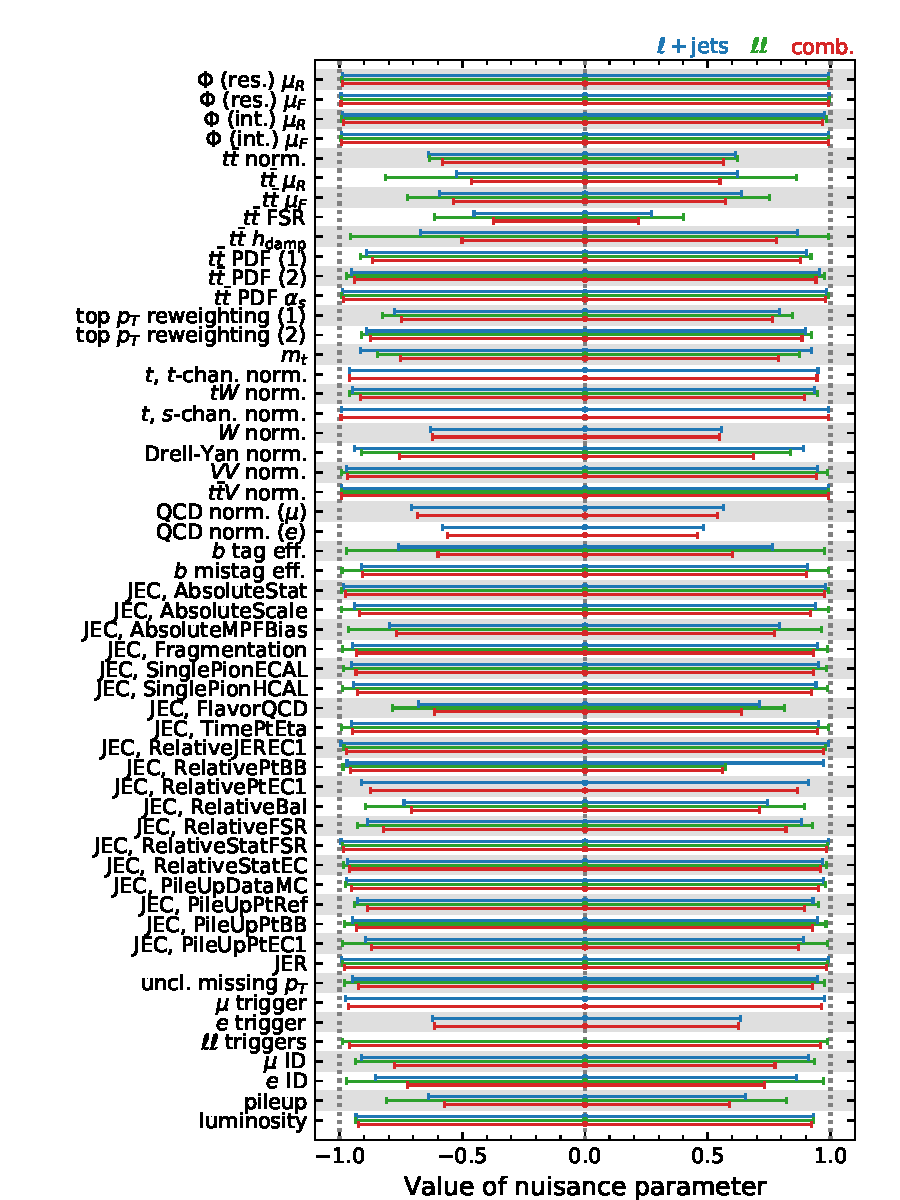
\includegraphics[width=0.85\textwidth,keepaspectratio=true]{fig/app5/impacts/constraints.pdf}
\caption{Constraints on nuisance parameters from a fit to the Asimov dataset, shown separately for the lepton-plus-jets (green) and the dilepton channel (red), and their combination (black).}
\label{fig:impacts_constraints}
\end{figure}

\begin{figure}[!Hhtb]
\centering
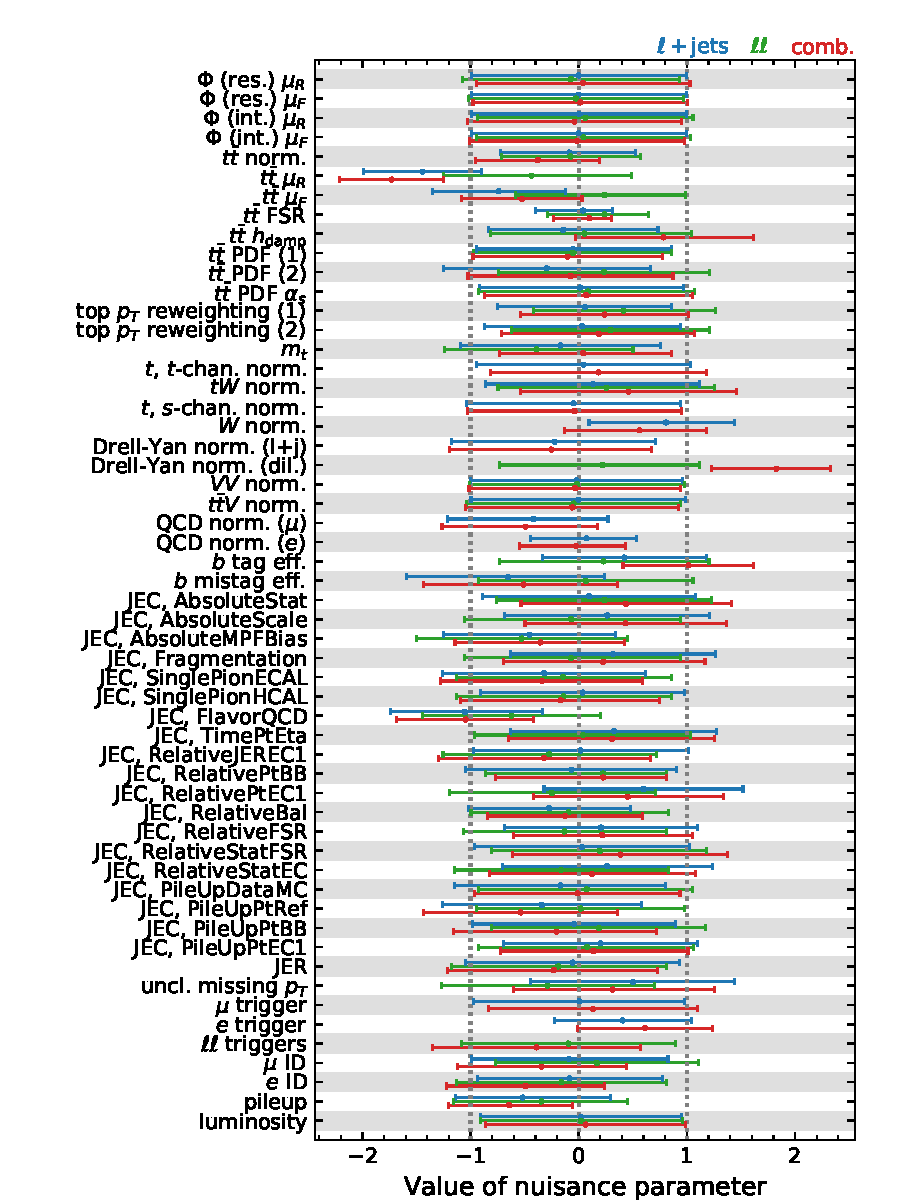
\includegraphics[width=0.85\textwidth,keepaspectratio=true]{fig/app5/impacts/constraints_unblind.pdf}
\caption{Constraints on nuisance parameters from a fit to datat, shown separately for the lepton-plus-jets (green) and the dilepton channel (red), and their combination (black).}
\label{fig:impacts_constraints_obs}
\end{figure}

Figures~\ref{fig:impacts_constraints} and ~\ref{fig:impacts_constraints_obs} show the expected and observed constraints on the nuisance parameters obtained from a fit to the Asimov dataset.
MC statistical uncertainties are not included.
\clearpage
\begin{figure}[!Hhtb]
\centering
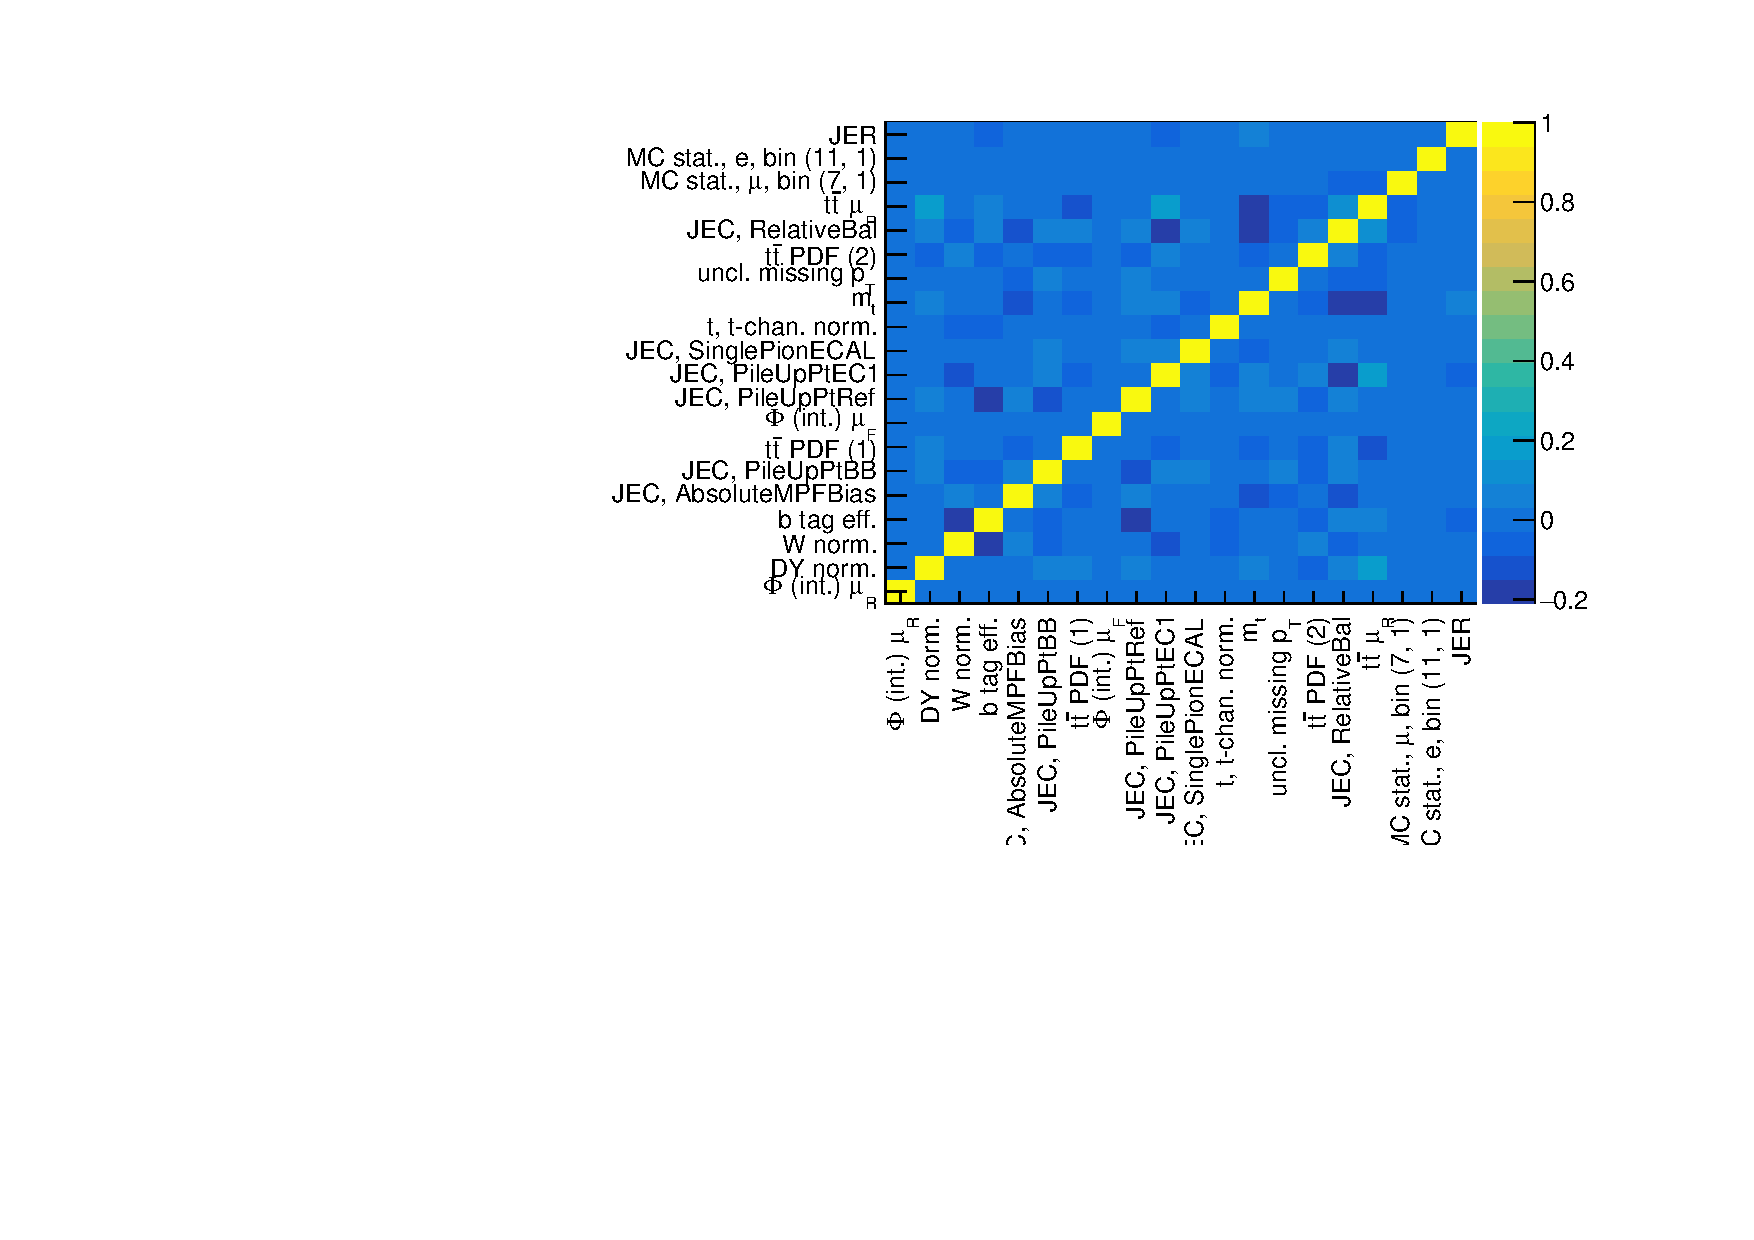
\includegraphics[width=0.85\textwidth,keepaspectratio=true]{fig/app5/impacts/correlation.pdf}
\caption{Correlations of 20 nuisance parameters with largest impact from a fit to the Asimov dataset. Both the correlations and the set of nuisance parameters with largest impacts are obtained using the benchmark point of $m_\mathrm{A} = 500$\,GeV and a relative width of 5\%.}
\label{fig:impacts_correlations}
\end{figure}

Figure~\ref{fig:impacts_correlations} shows the correlations of the 20 nuisance parameters with largest impact, obtained from a fit using $m_\mathrm{A} = 500$\,GeV and a relative width of 5\%, and the signal strength corresponding to the central expected limit. 

\clearpage{\pagestyle{empty}\cleardoublepage}
